\chapter{Design and evaluation of the Paper Prototype}


This chapter describes the design and the evaluation of the paper prototype. The design was done on paper and with the knowledge of usability issues in mind. The existing approaches of eco-feedback applications have been evaluated in the section~\ref{sec:approaches}. Especially the design principles were the basis for the hand-sketched drafts. The evaluation was done in a paper prototype session with the users found with the questionnaire. The workshops were held not only done to test usability but first and foremost to answer 

\textbf{RQ 4: Do the characteristics of user groups correlate with the users' preferred type of visualization?}

The mobile application of ASCR will be investigated in particular and will be the basis for the paper prototypes.

As described before in \ref{section:paperprototyping} we follow the Step-by-Step guide of Arnowitz et al. \cite{arnowitz2010effective} to create a Paper Prototype. The first task of the Step-by-Step guide is to define the tasks in a scenario narration.

\textbf{Scenario narration} \quad The main goal of the mobile application for which the paper prototype is sketched is to give eco-feedback. This feedback shall primarily focus on the consumption of electricity, water and heating and the emission of carbon-dioxide. So the history consumption rate of these data shall be available to look into. A comparison of the consumption during different time intervals shall also be possible. This comparison can be drawn to one's own consumption but also to a comparable household, to an average consumption rate of the neighbours, the city or the European Union. On a dashboard the current measured values, the consumption of the day and some current settings shall be shown. The management of the home automation system shall also be available via the app. Tips for saving money by saving energy shall also be given. Energy saving-tips shall be tailored to the characteristics of a user type. Especially for Hedonists the menu item "Project" will be interesting. Here projects are listed, which show possible further home automation items that can help at energy saving. A user can read frequently asked questions in the FAQ section.

\section{Design of Paper Prototype}
Having in mind the above mentioned tasks we designed multiple versions of the paper prototypes that resulted from several runs through the Step-by-Step guide for the creation of a paper prototype of Arnowitz et al. \cite{arnowitz2010effective}. The outcomes of these process are described below. For better readability we describe the user interfaces followed by the results of the paper prototyping sessions.

\section{Menu navigation}

We developed a navigation drawer and adapted it to the requirements of each user type, as shown in Figure ~\ref{fig:drawer}. The sorting of the menu items was adapted to the main motivation why a user uses the app.

\textbf{Improvements} \quad The test user from the Optimizer and Indifferent user section stated that a drag and drop function to resort the items would be a nice-to-have feature. One Optimizer suggested to use a different colour for each menu item to make it visually more appealing. Also the use of icons was highly recommended.

\begin{figure}[h]
	\centering
	\begin{subfigure}[b]{0.24\columnwidth}
		\centering
		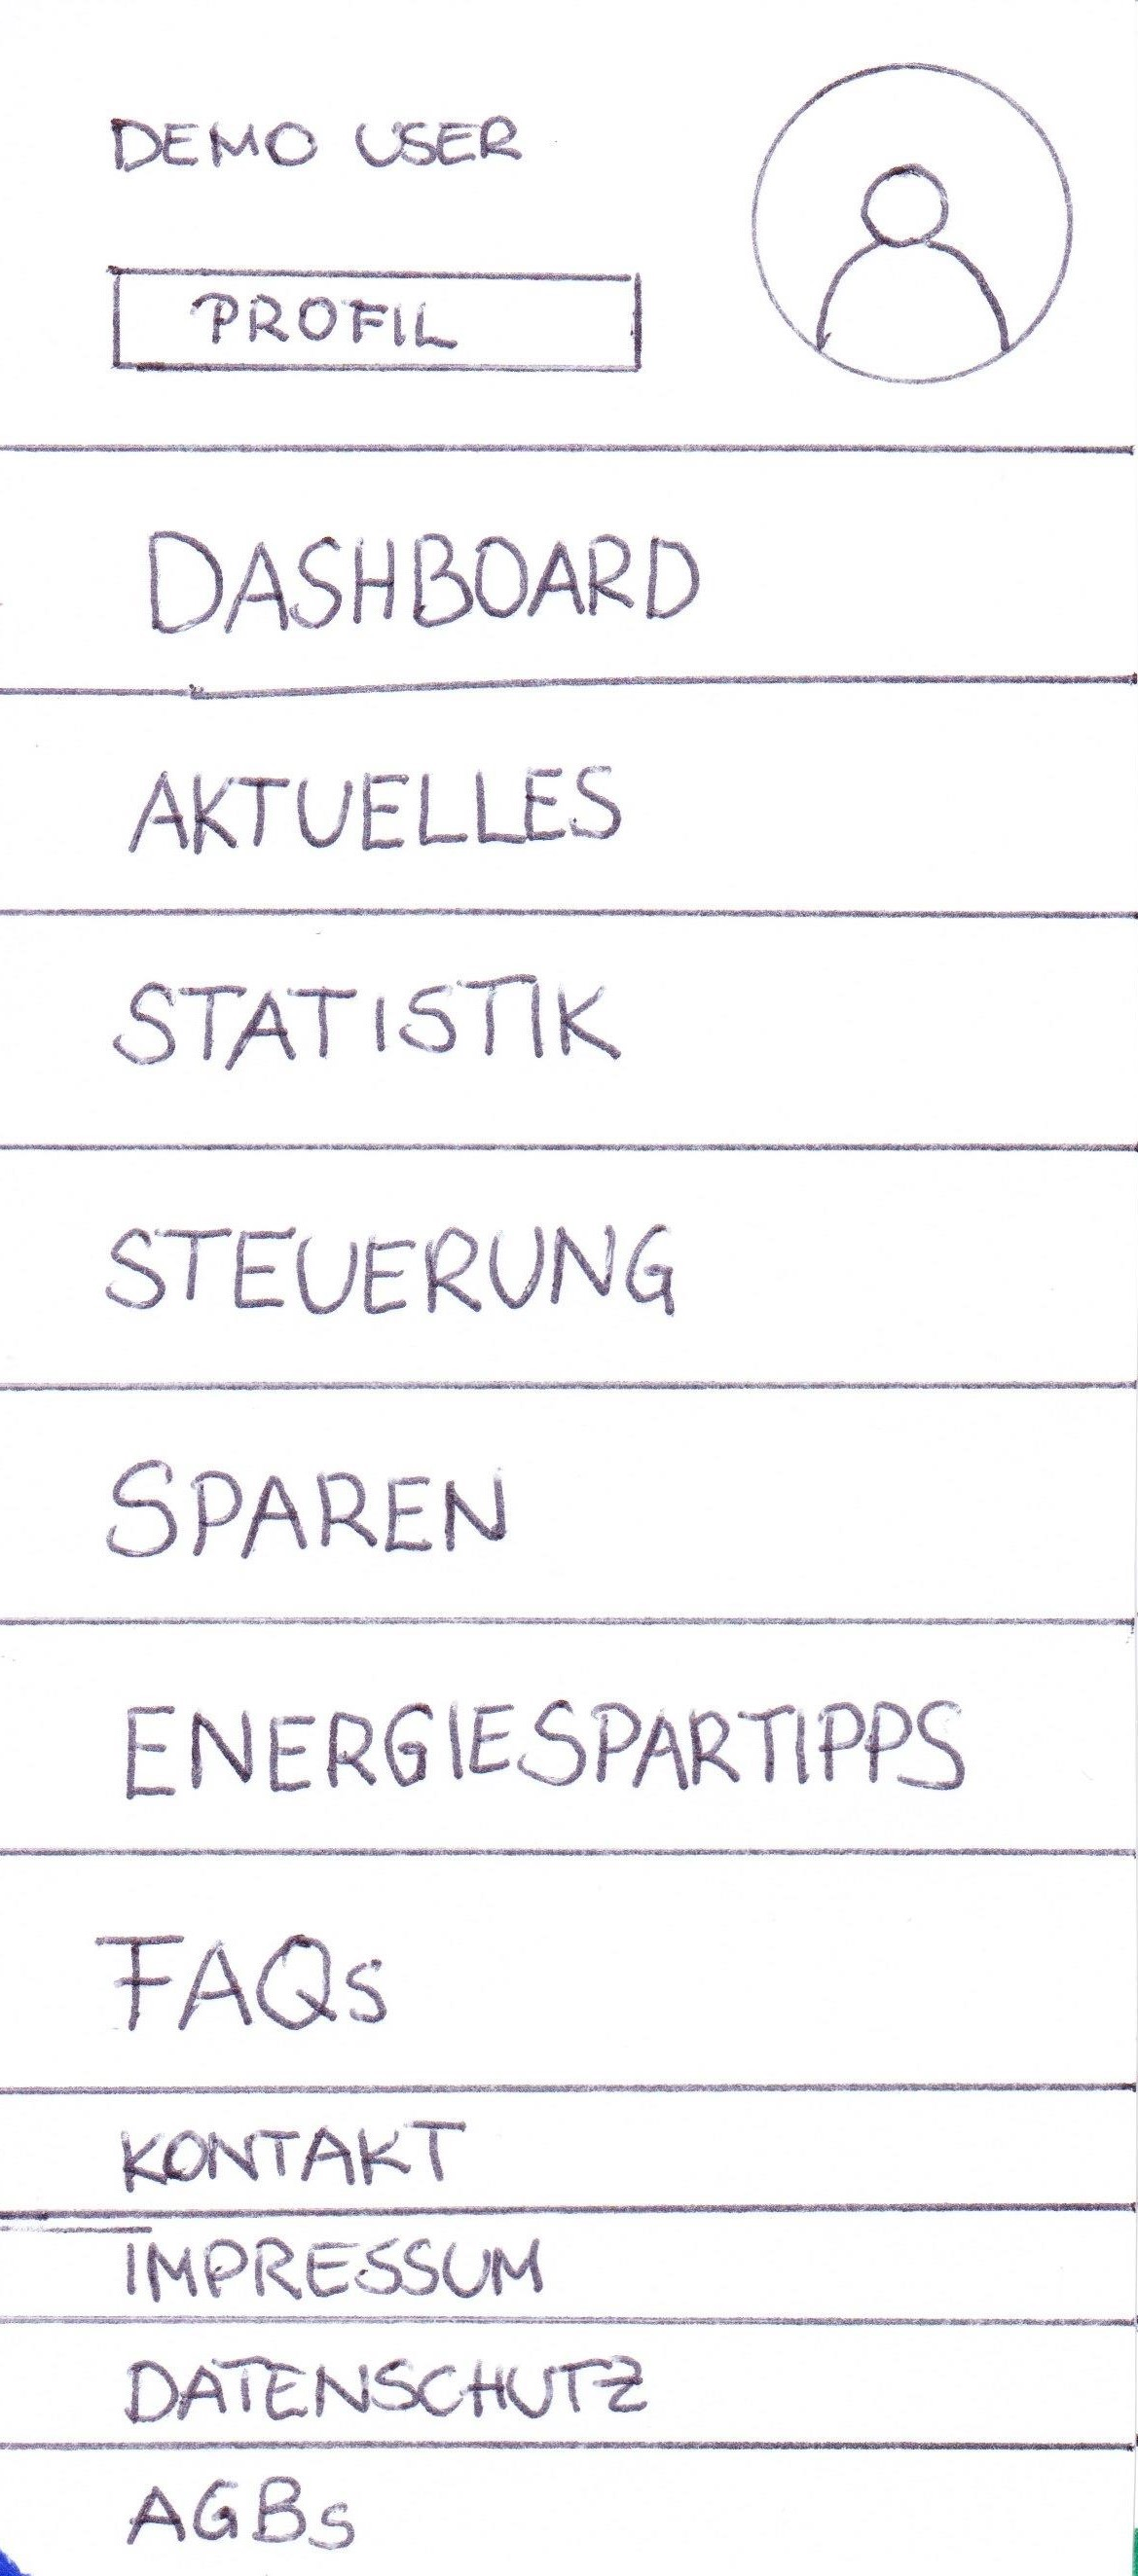
\includegraphics[width=\textwidth]{screens/drawer_1}
		\subcaption{Professional}
		\label{fig:drawer:professional}
	\end{subfigure}
	\begin{subfigure}[b]{0.24\columnwidth}
		\centering
		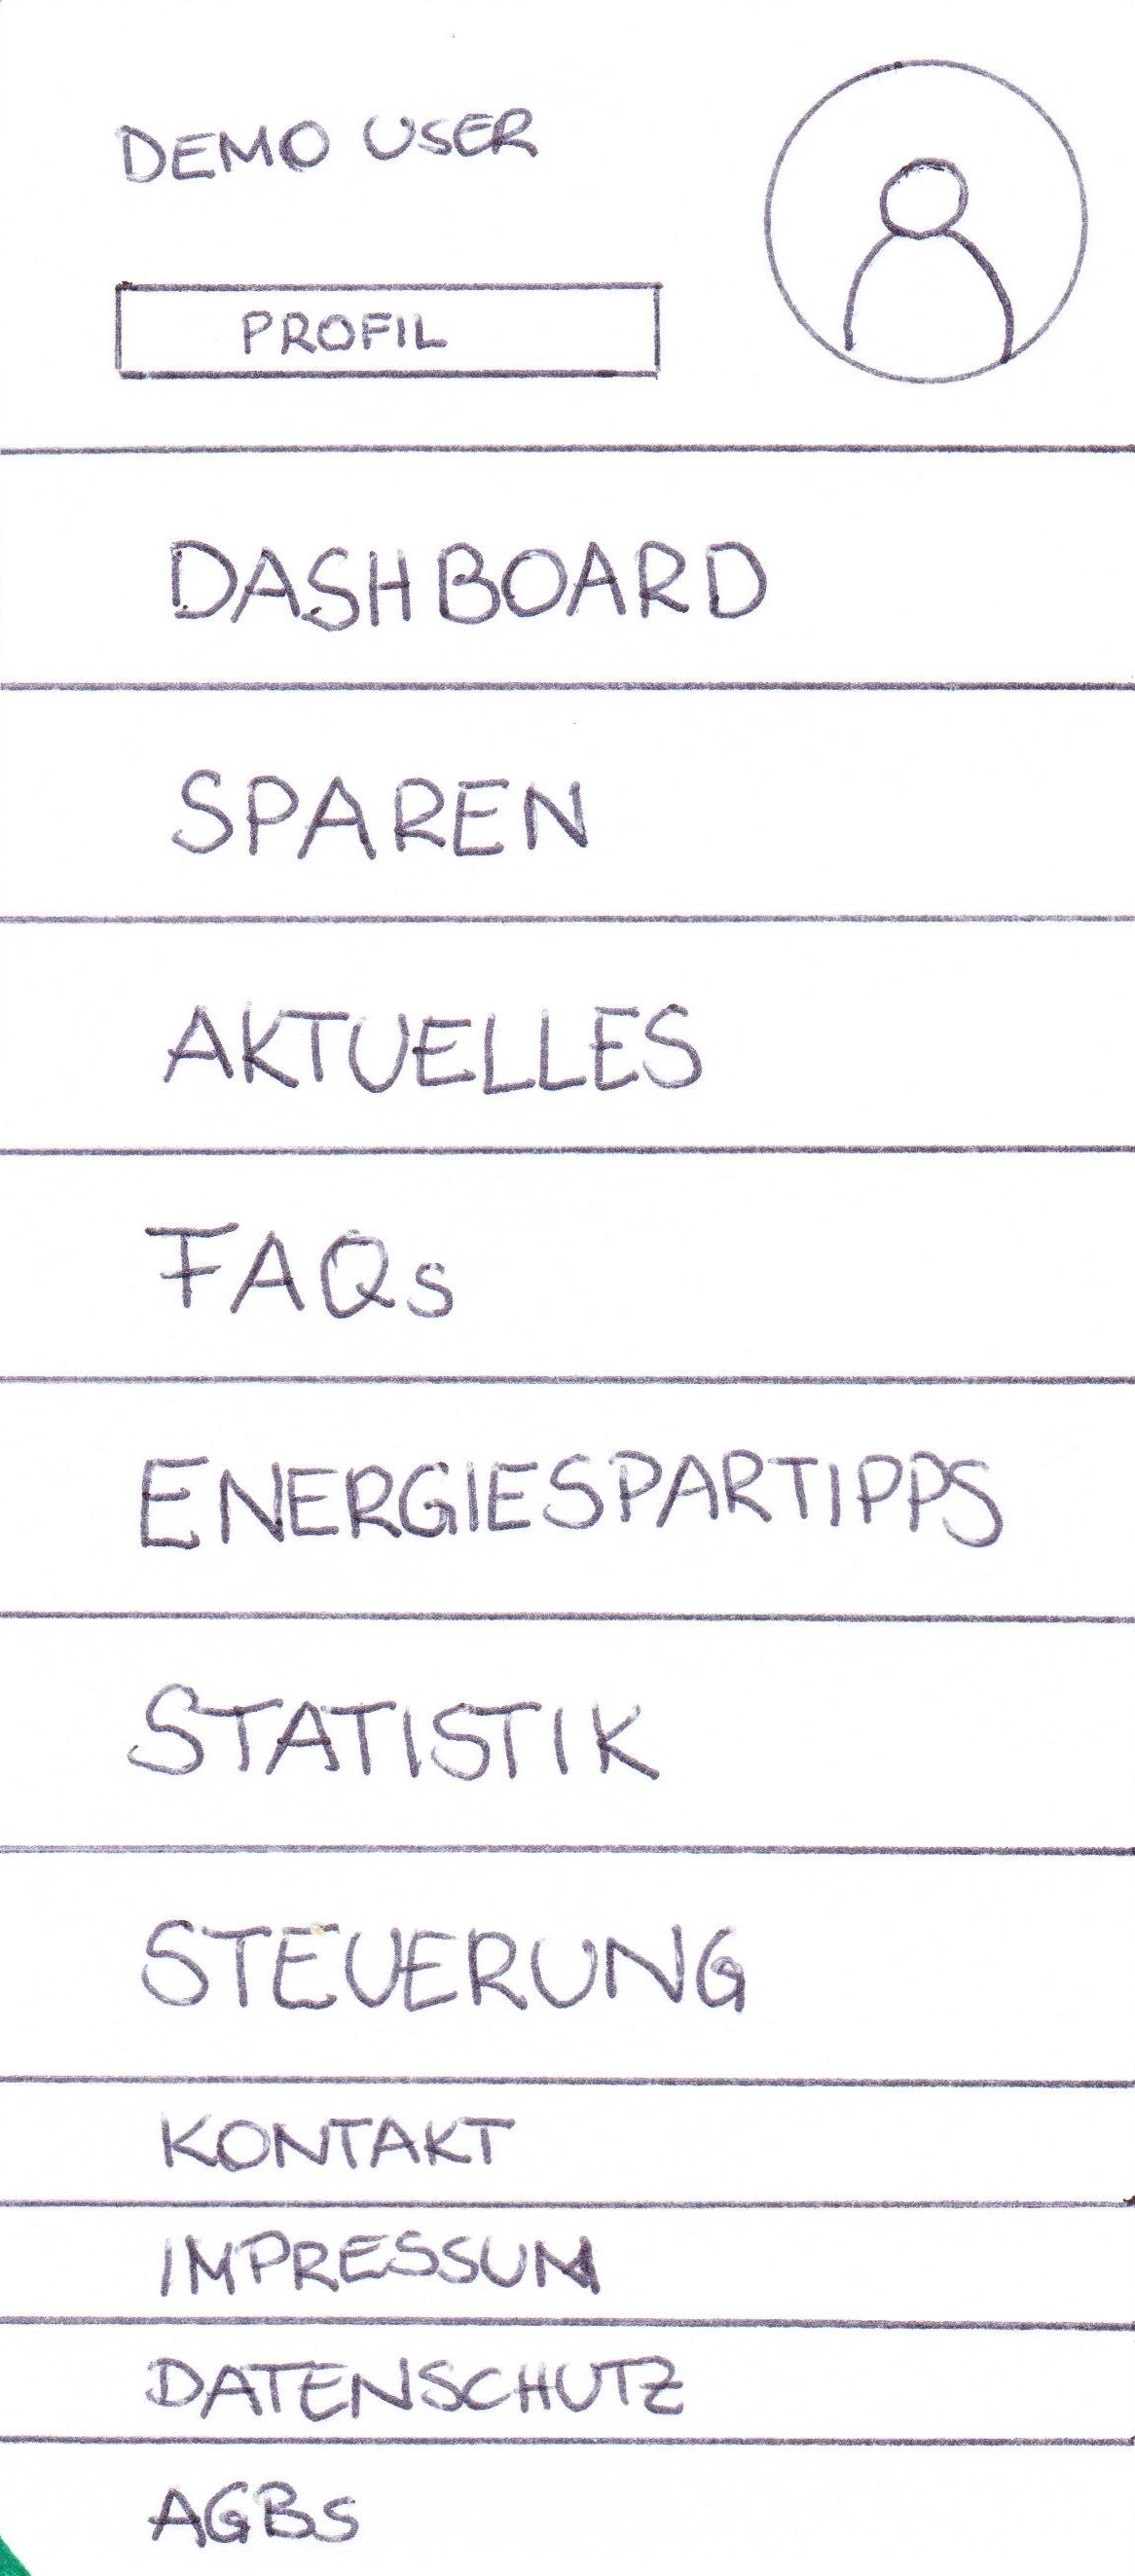
\includegraphics[width=\textwidth]{screens/drawer_2}
		\subcaption{Optimizer}
		\label{fig:drawer:optimizer}
	\end{subfigure}
	\begin{subfigure}[b]{0.24\columnwidth}
		\centering
		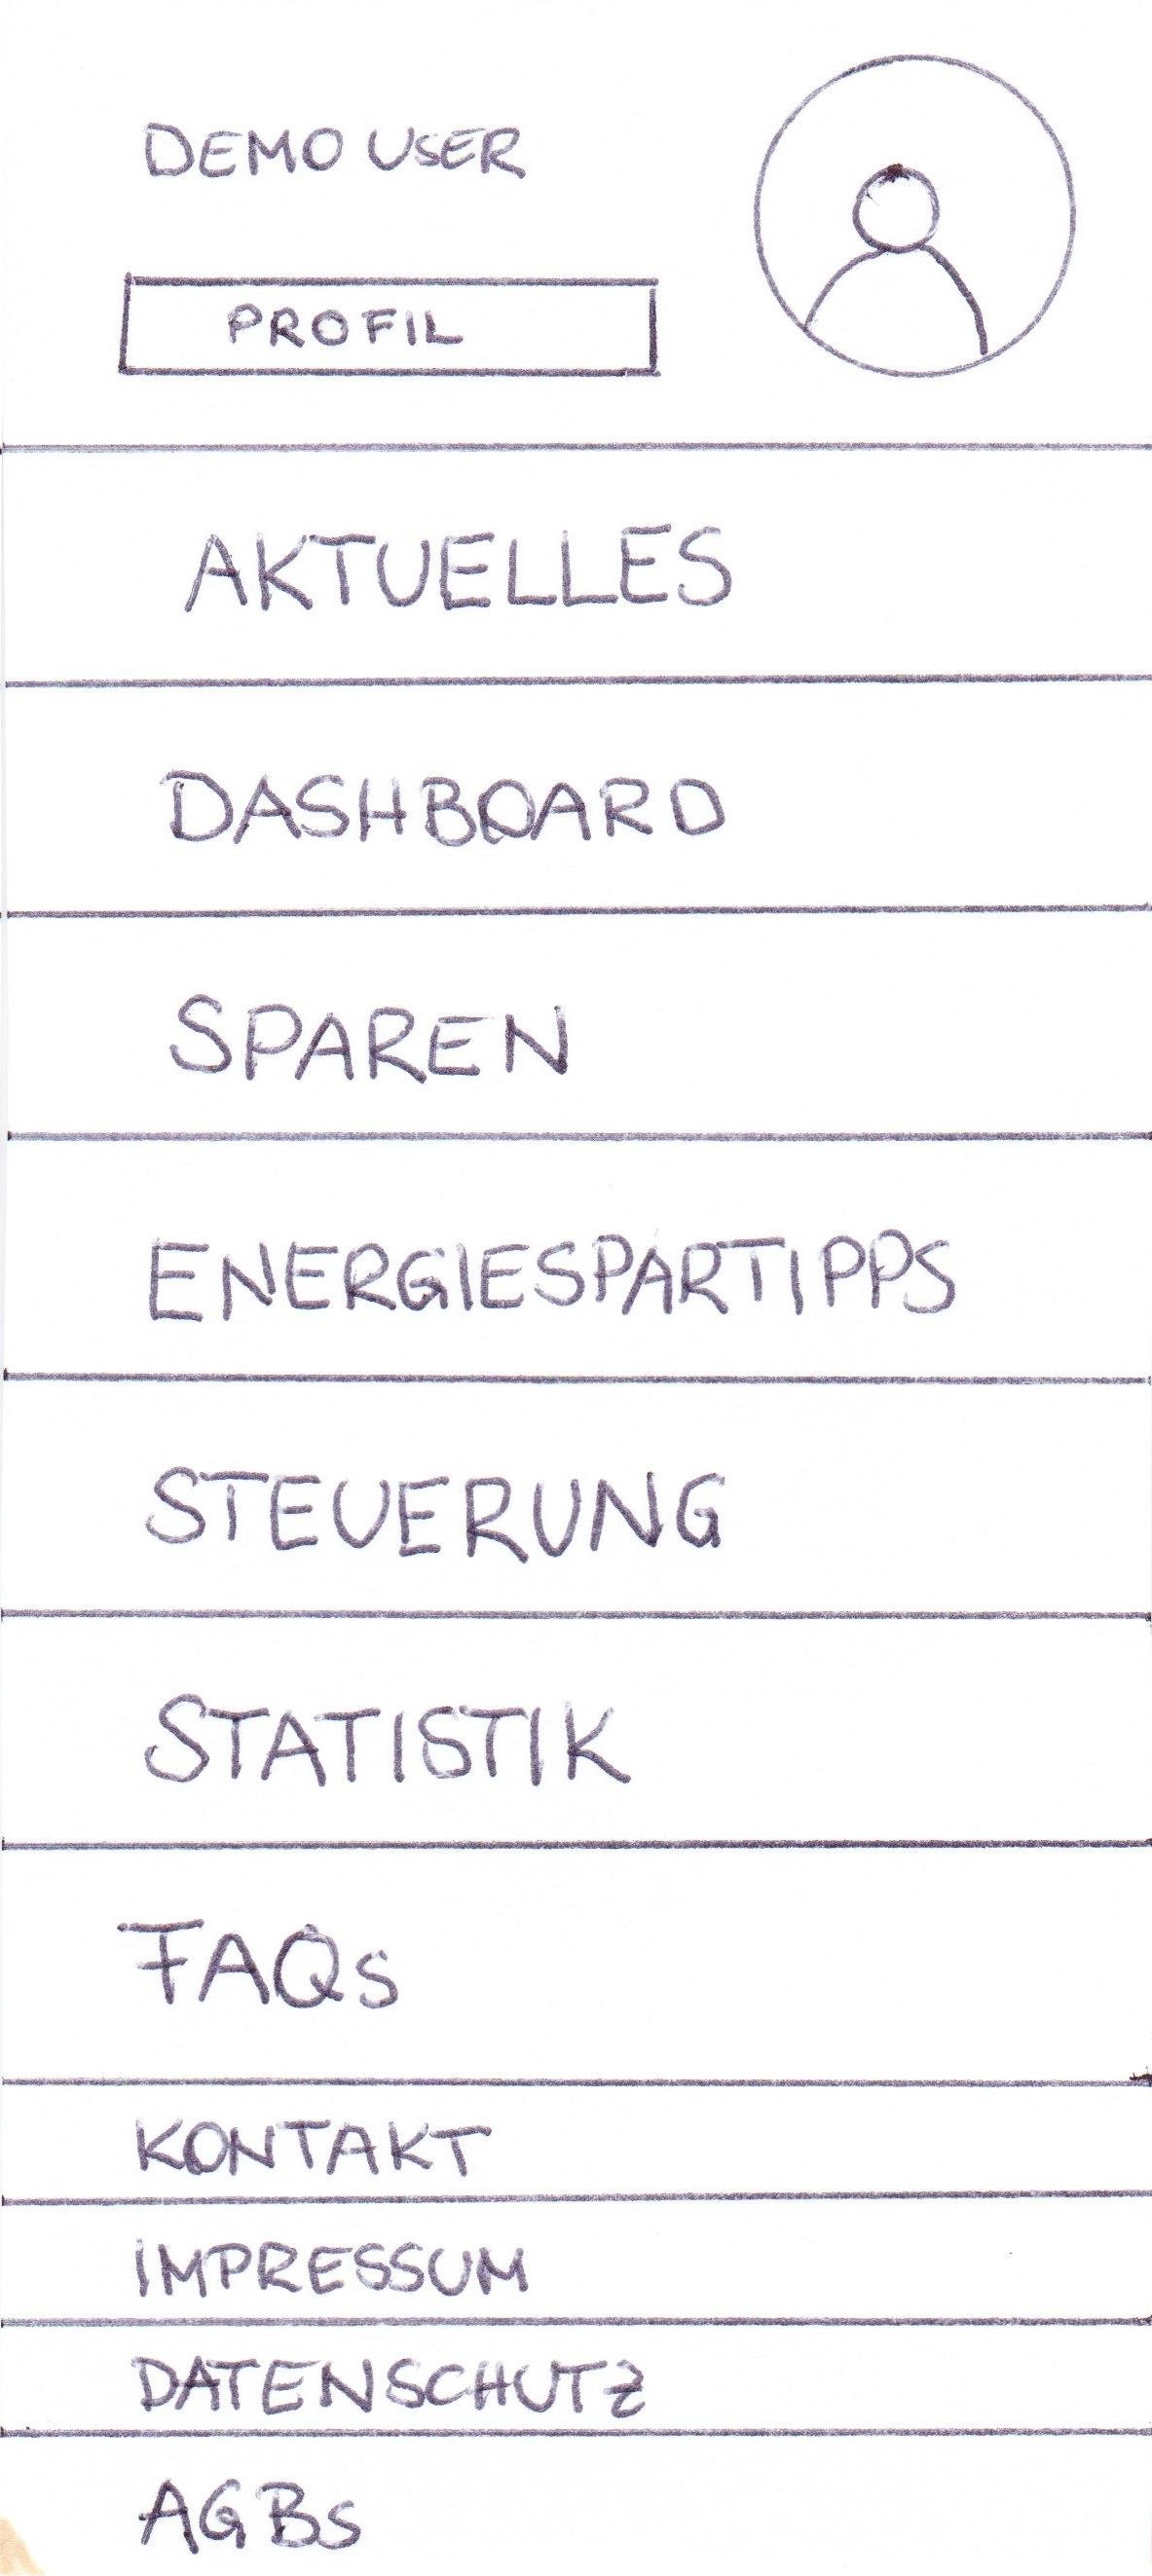
\includegraphics[width=\textwidth]{screens/drawer_3}
		\subcaption{Indifferent}
		\label{fig:drawer:indifferent}
	\end{subfigure}
	\begin{subfigure}[b]{0.24\columnwidth}
		\centering
		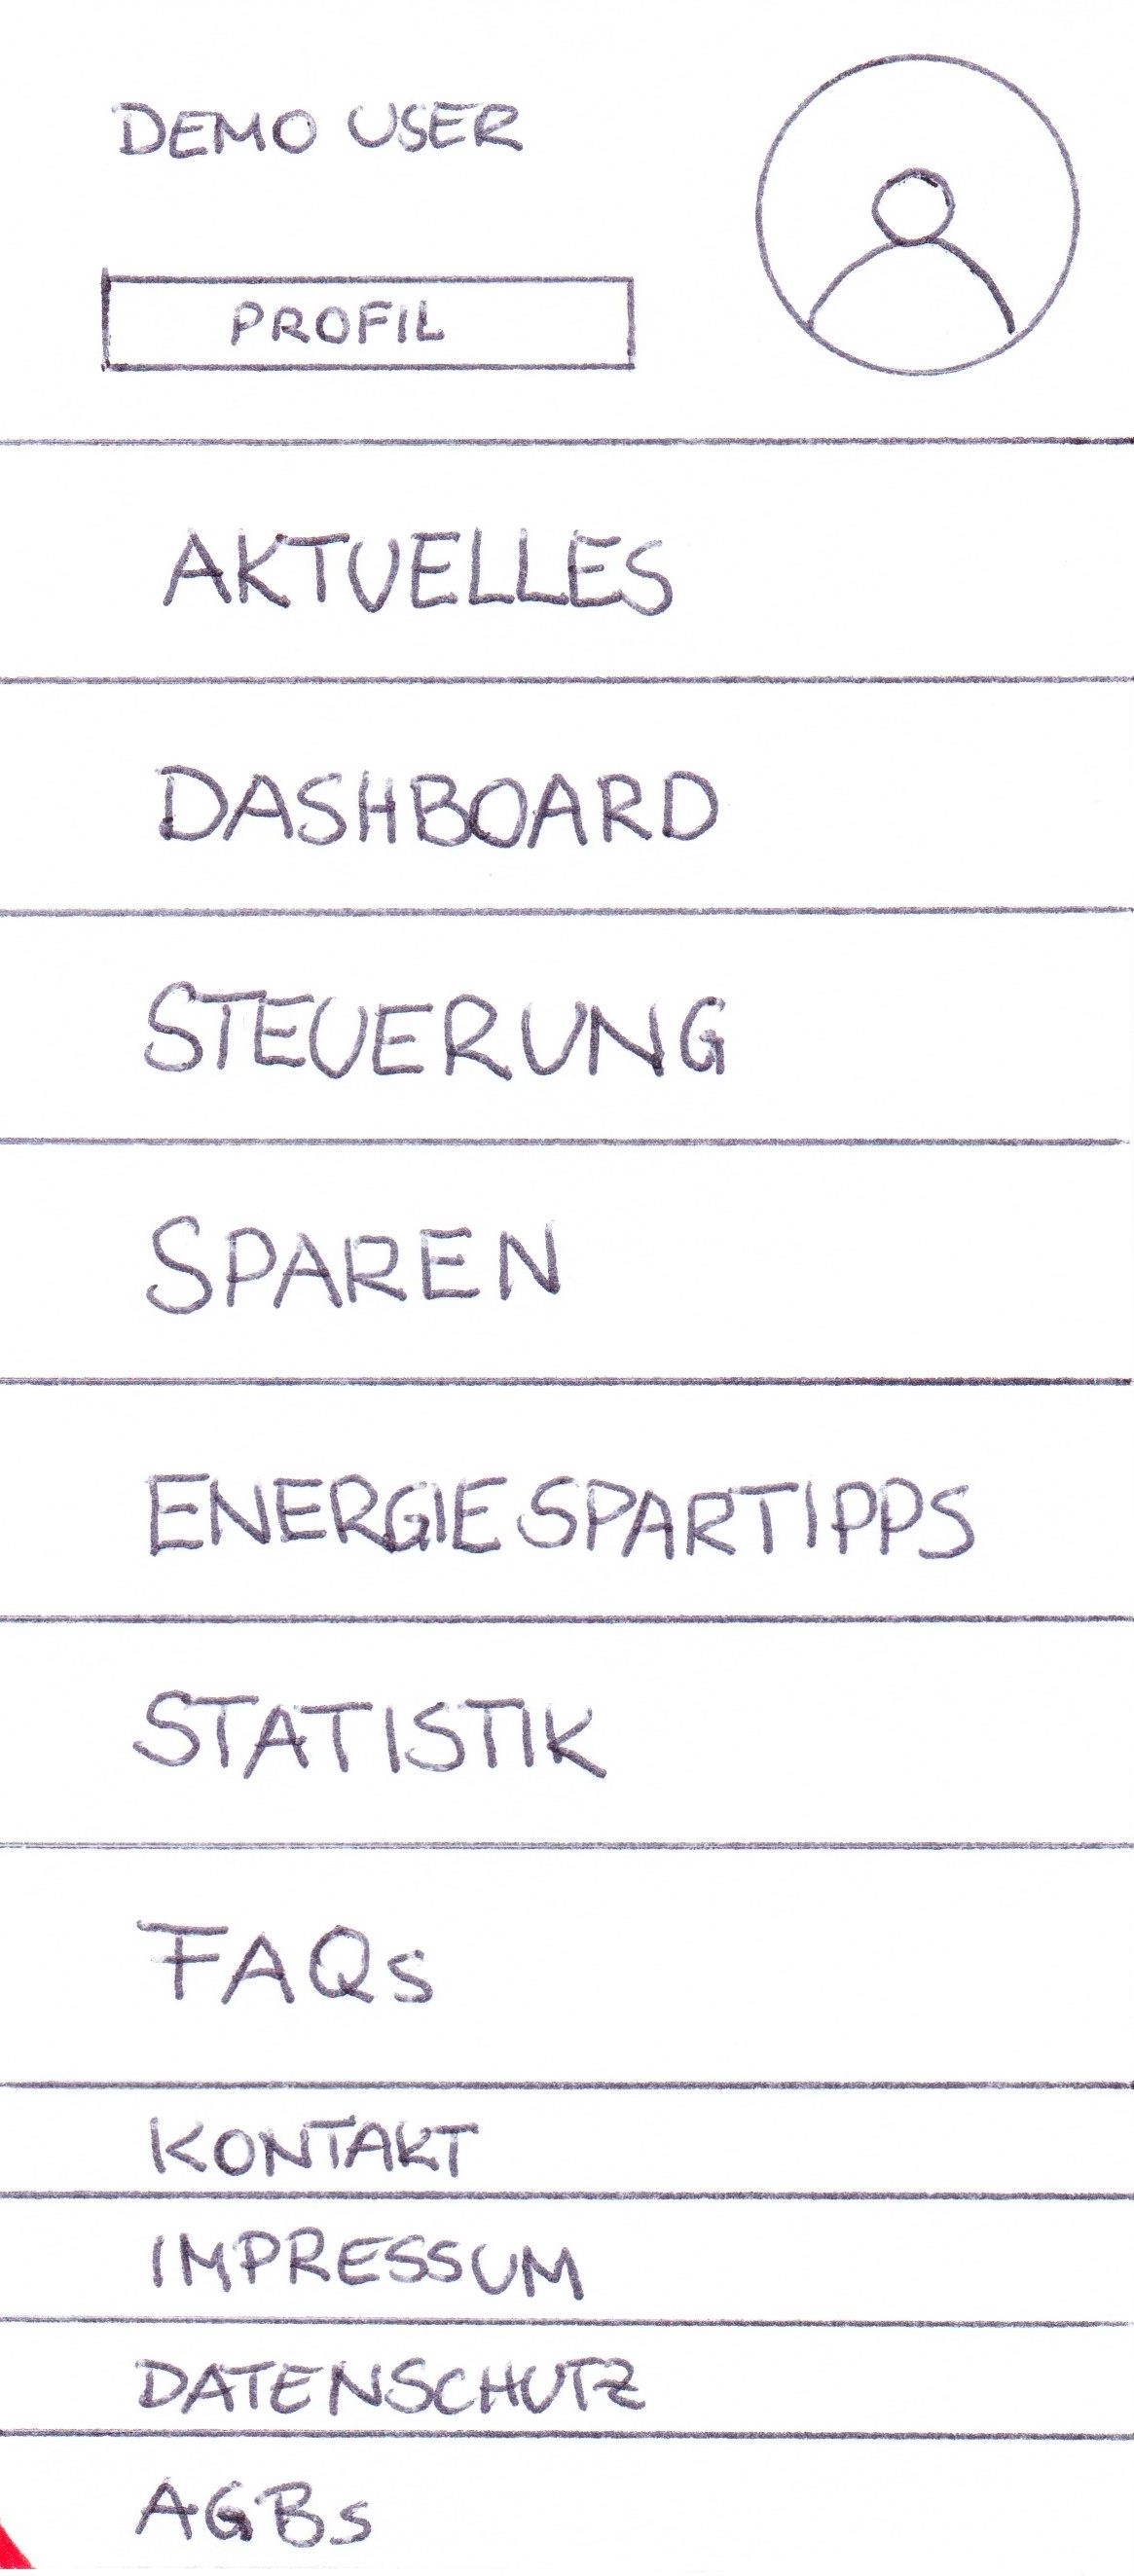
\includegraphics[width=\textwidth]{screens/drawer_4}
		\subcaption{Hedonist}
		\label{fig:drawer:hedonist}
	\end{subfigure}
	\caption{Proposed screens for the navigation drawer}
	\label{fig:drawer} % \label has to be placed AFTER \caption (or \subcaption) to produce correct cross-references.
\end{figure}


\subsection*{Guideline 1: Adapt navigation drawer to requirements of user type}

 Sort the items of the navigation drawer according to the motivation of a user type. An effect would be that a user can quickly interact with the app as the preferred items are on top. The sorting reduces the time a user has to search for his/her primary task. However, the different sorting can be irritating when a user compares the app to a user who is a different type of energy user and therefore has another look of the app.
 
\textbf{Evidence} \quad The paper prototype session with the professionals has shown that Professionals primarily use the app for monitoring their consumption rate, therefore the Dashboard is the first menu item. The main motivation for Optimizer is to save money with the app. Indifferents primarily use the app because it makes fun which means that their main motivation is supported by the gamification approach. Hedonists' are especially motivated to use the app, when their drive for programming projects is picked up. The gamification approach and the projects are shown in the first menu item, for that reason the Dashboard is on second place for Hedonists and Indifferents. The following user stories were tested in the paper prototype session with the according user types and were proven to appropriate:
\begin{itemize}
	\item As a Professional I primarily use the app to monitor my consumption rate.
	\item As an Optimizer I primarily use the app to save money
	\item As an Indifferent I primarily use the app for fun
	\item As a Hedonist I primarily use the app to manage my home automation gadgets	
\end{itemize}


\section{Measurements}

The dashboard was based on the one from the ASCR application. As visible in~\ref{fig:dashboard}, the main difference is the use of kWh for Professionals and Hedonists and the use of Euro for Optimizer and Indifferents. Especially the scale of the air humidity was stated as appealing from the test users.

\textbf{Evidence} \quad One critic from a Professional was, that the screen misses, how the quality of the air can be improved. Grouping the measured values to one side and the values that can be controlled to the other side was also suggested by a Professional. The Optimizer again wished for more colours and symbols. A similar scale for CO2 as for the air humidity was mentioned by the Indifferent segment of test users. An extra pop up window for the adjustable values was desired from the Hedonist test user.

\begin{figure}[h]
	\centering
	\begin{subfigure}[b]{0.24\columnwidth}
		\centering
		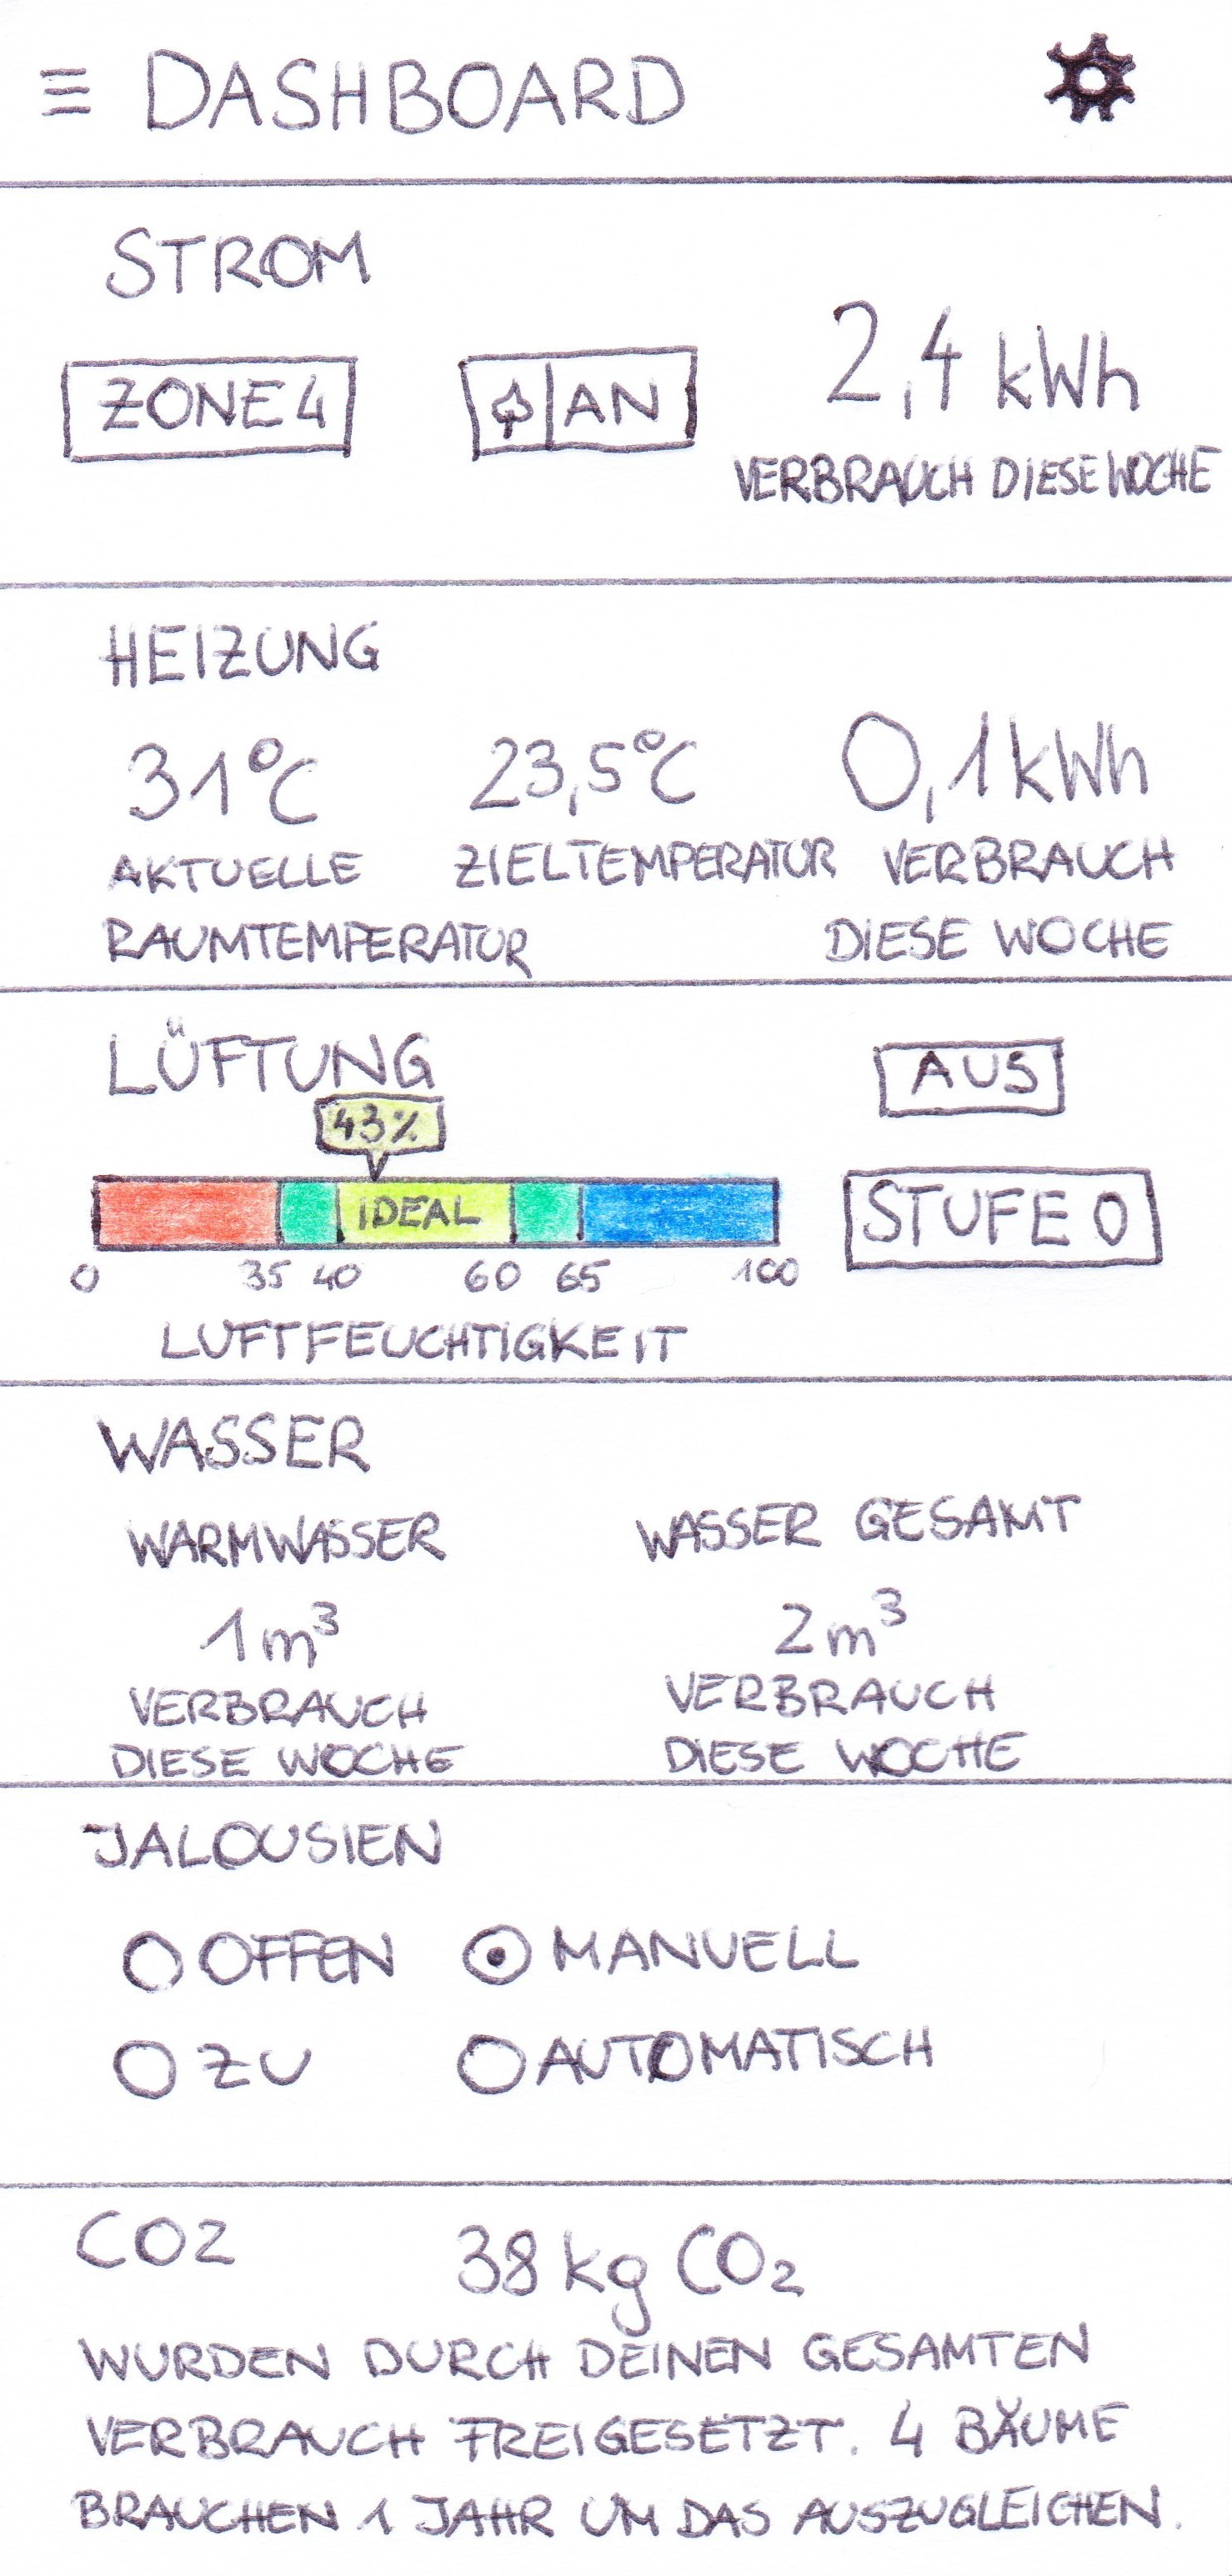
\includegraphics[width=\textwidth]{screens/dashboard_14}
		\subcaption{Professional and Hedonist}
		\label{fig:dasboard:professional}
	\end{subfigure}
	\begin{subfigure}[b]{0.24\columnwidth}
		\centering
		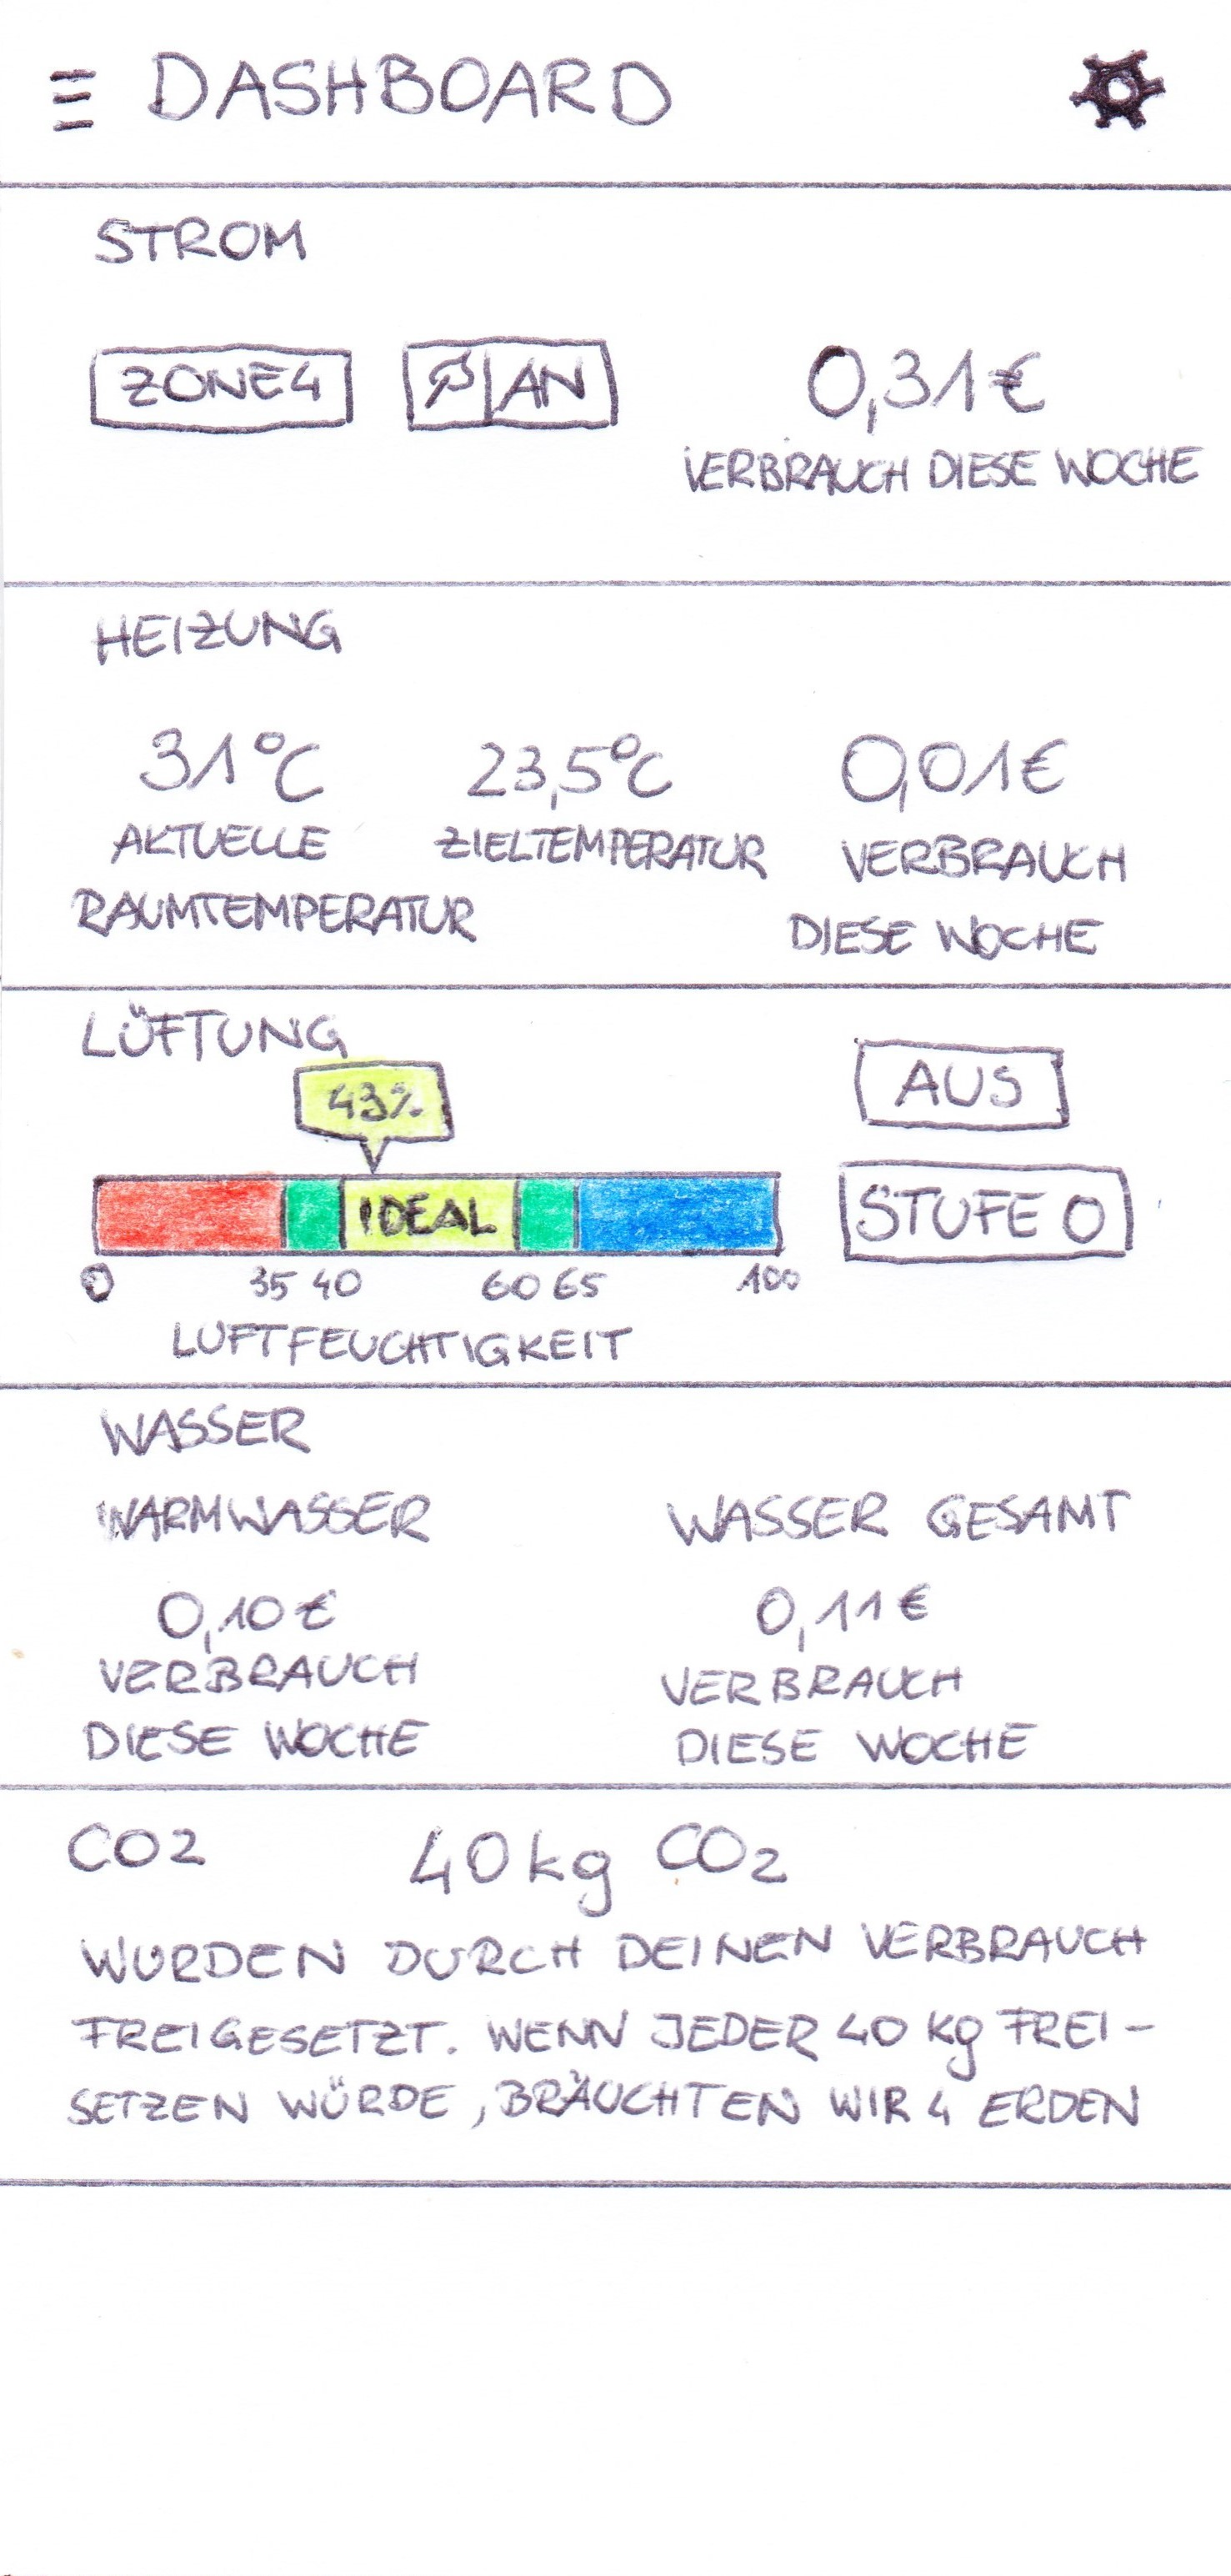
\includegraphics[width=\textwidth]{screens/dashboard_23}
		\subcaption{Optimizer and Indifferent}
		\label{fig:dashboard:optimizer}
	\end{subfigure}
	\caption{Sketches of the dashboard}
	\label{fig:dashboard} % \label has to be placed AFTER \caption (or \subcaption) to produce correct cross-references.
\end{figure}

\subsection*{Guideline 2: Use monetary units for Optimizers and Indifferents and units of energy or consumption for Professionals and Hedonists}

Depending on the user type the measurement unit is changed and the value converted accordingly. The electricity and heating consumption is shown in kWh for Professionals and Hedonists and in Euro for Optimizers and Indifferents. The same counts for consumption of water. Optimizers and Indifferents prefer the measurement unit Euro to cubic meter.

\textbf{Evidence} \quad Tailoring, as mentioned before in ~\nameref{subsec:primaryTask}, is beneficial for persuasion. The tailoring of the measurement unit to the preferences was defined as very beneficial by all user types. It was very clear in all testing sessions that the proposed unit for the particular user group was preferred. The following user stories were shown to be true: 

\begin{itemize}
	\item As a Professional I prefer units of energy or consumption to monetary units
	\item As an Optimizer I prefer monetary units to units of energy or consumption
	\item As an Indifferent I prefer monetary units to units of energy or consumption
	\item As a Hedonist I prefer units of energy or consumption to monetary units
\end{itemize}

\section{Latest topics}

In the latest topics section a user can see informations that are daily new. Professionals and Hedonists are given the project item and Optimizer and Indifferents have the 

\begin{figure}[h]
	\centering
	\begin{subfigure}[b]{0.24\columnwidth}
		\centering
		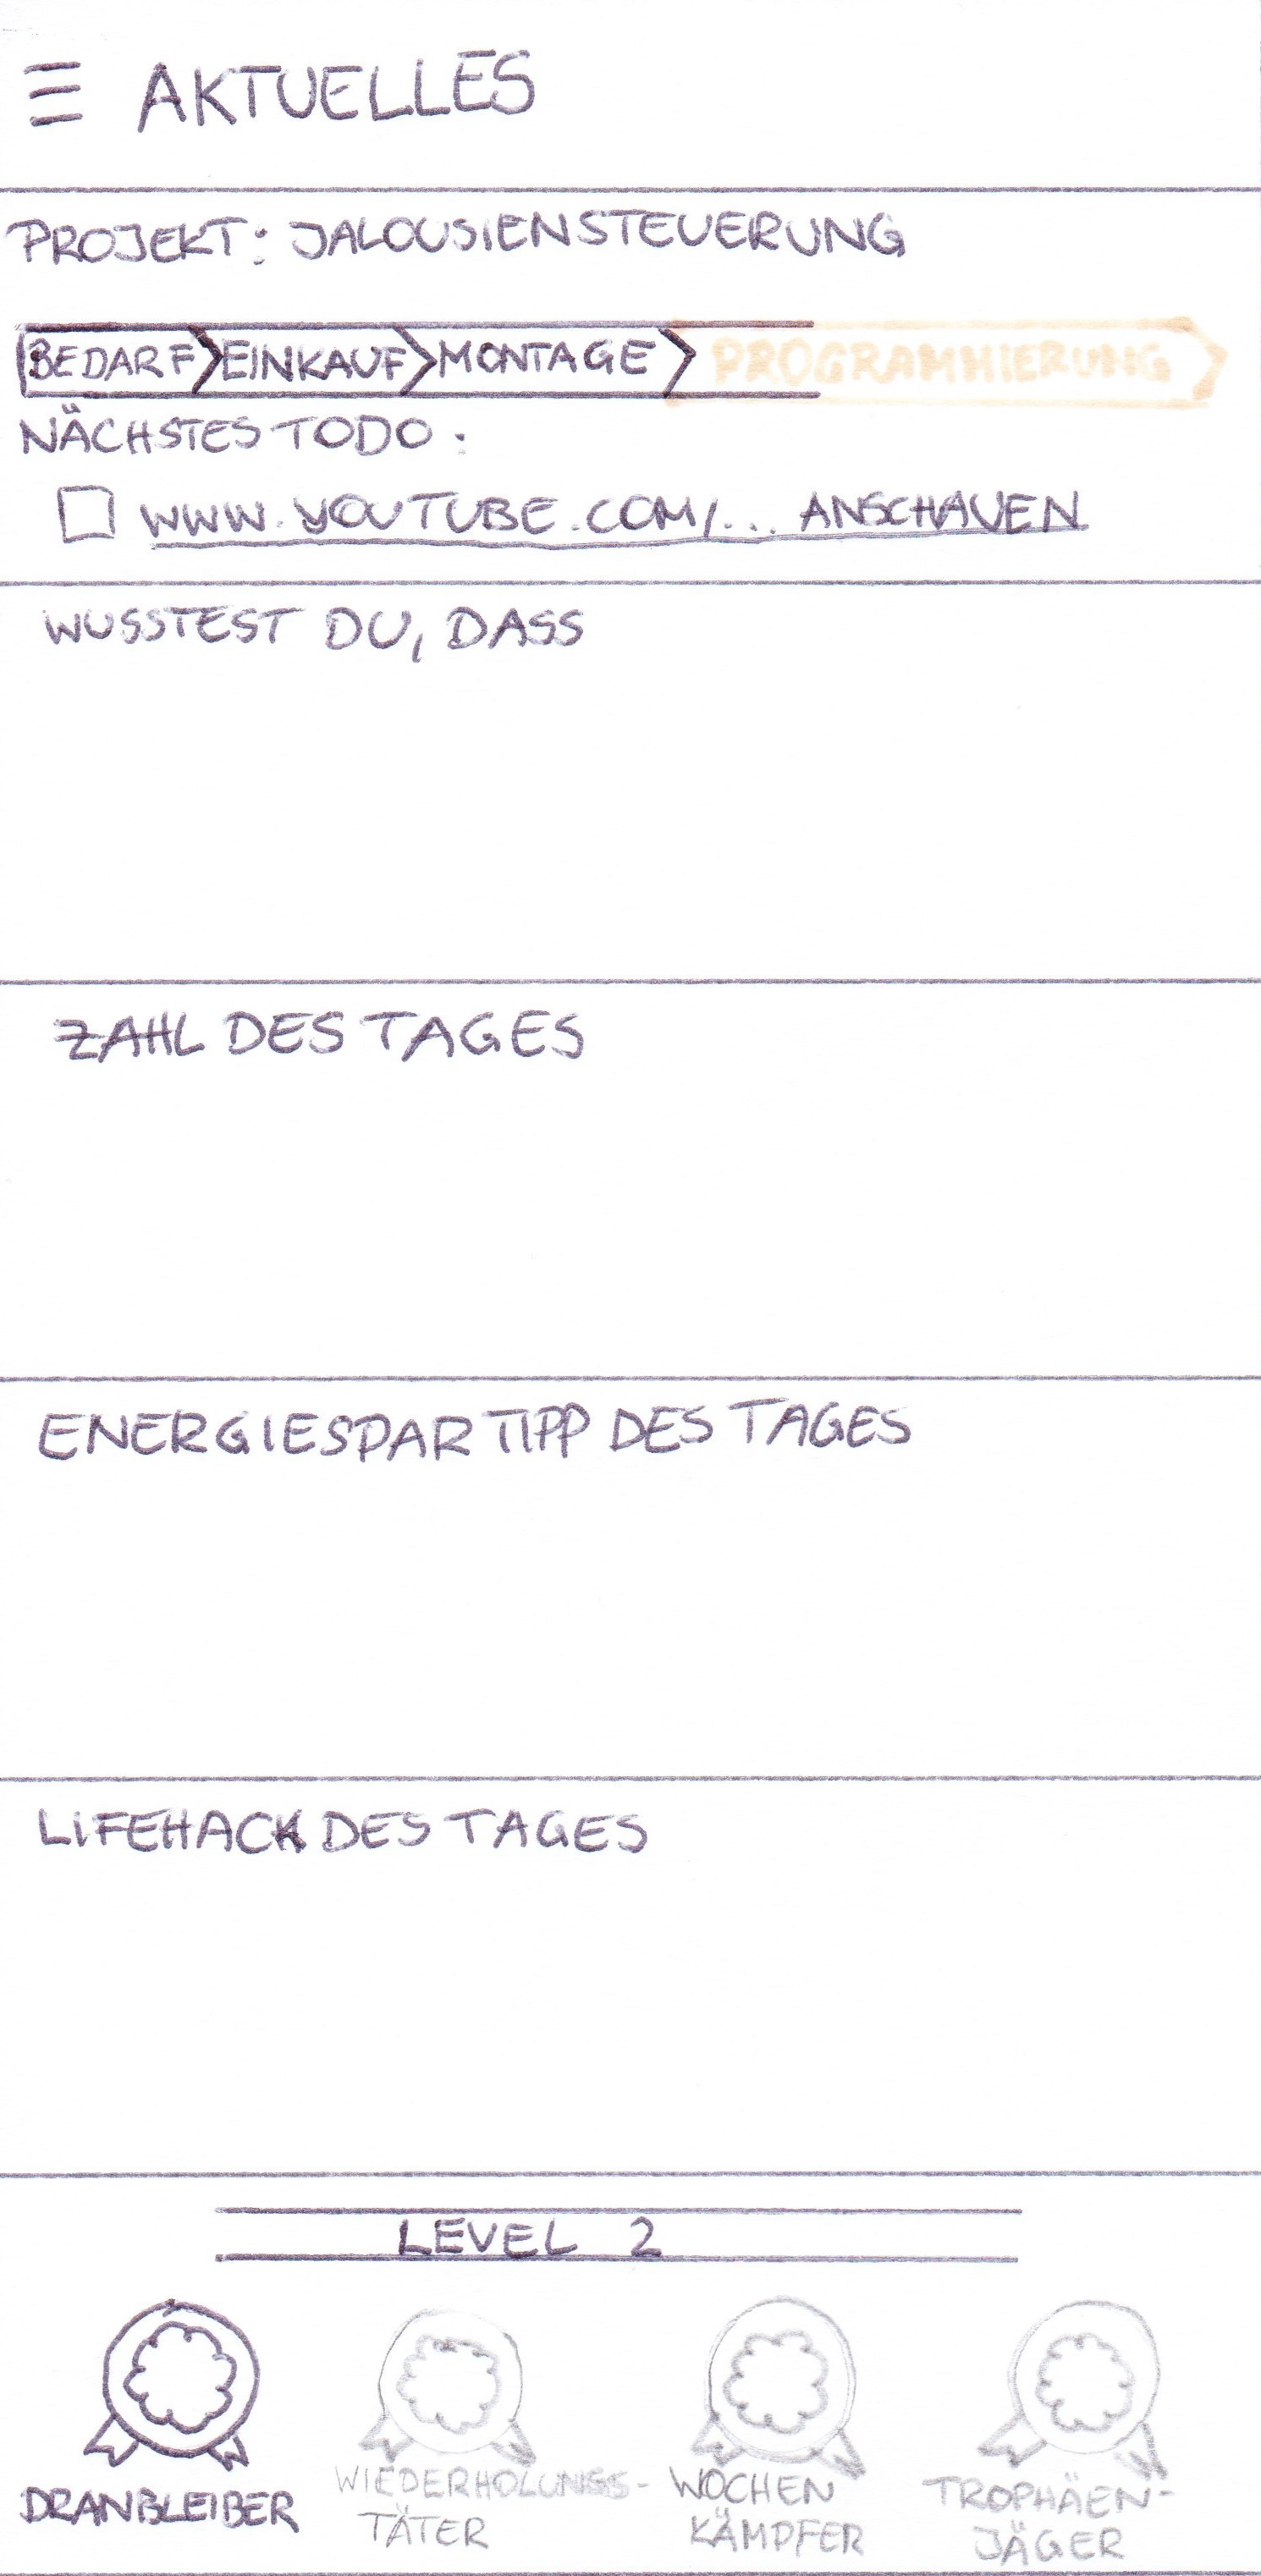
\includegraphics[width=\textwidth]{screens/aktuelles_14}
		\subcaption{Professional and Hedonist}
		\label{fig:aktuelles:professional}
	\end{subfigure}
	\begin{subfigure}[b]{0.24\columnwidth}
		\centering
		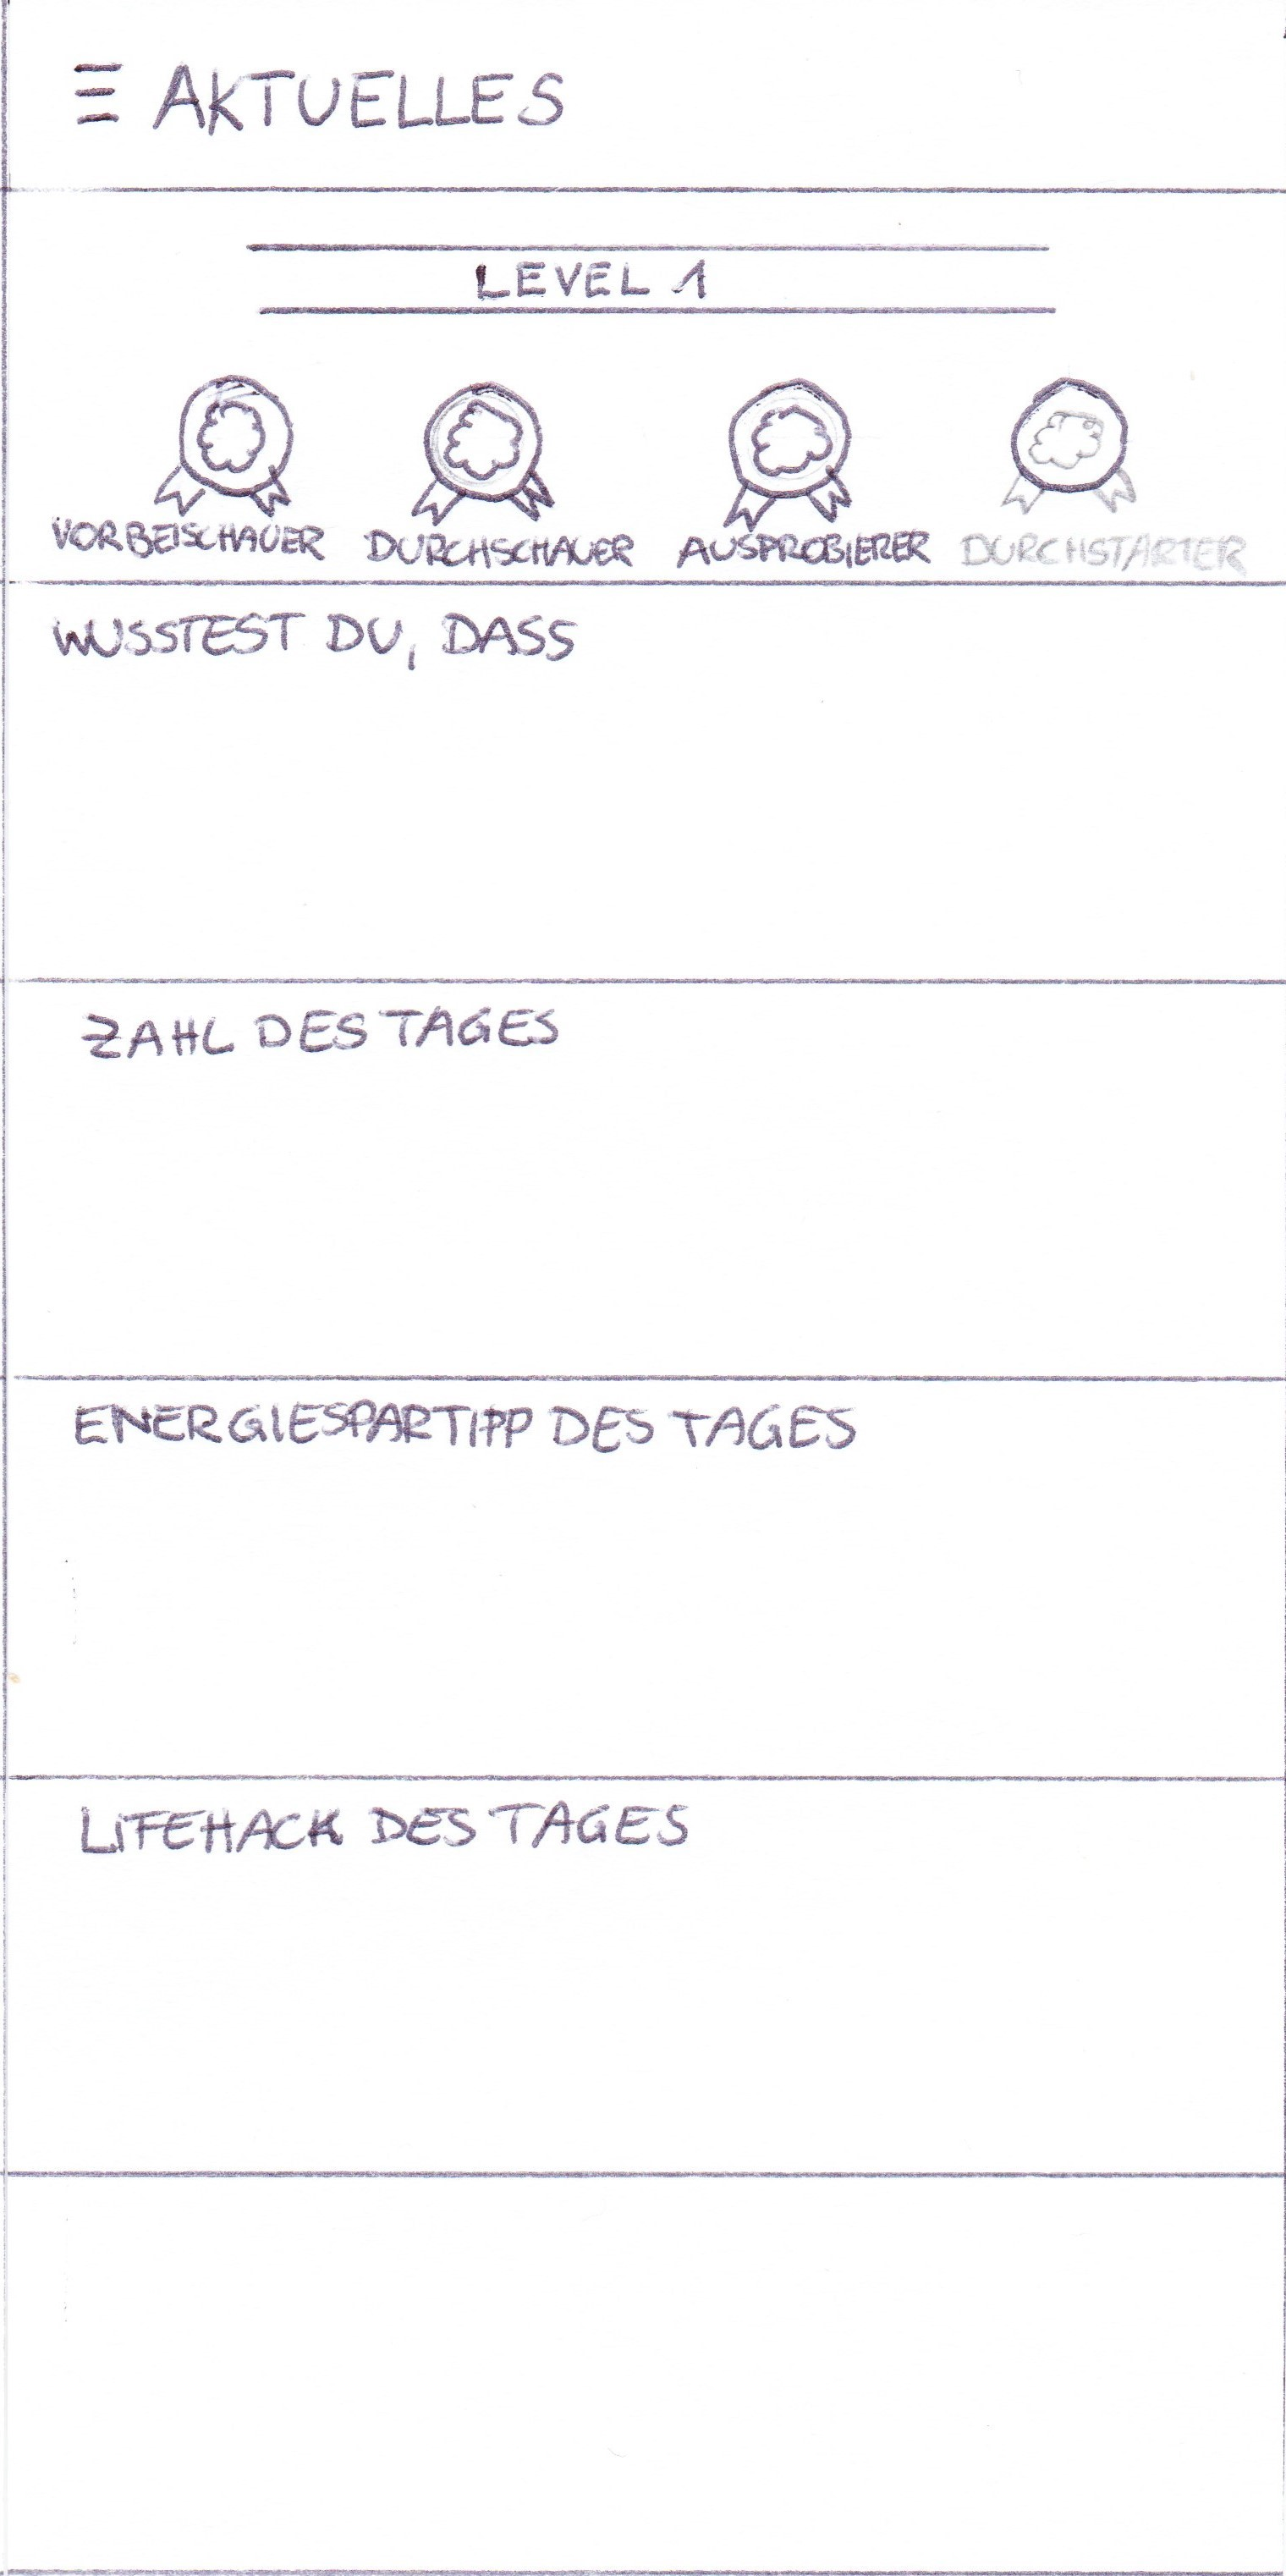
\includegraphics[width=\textwidth]{screens/aktuelles_23}
		\subcaption{Optimizer and Indifferent}
		\label{fig:aktuelles:optimizer}
	\end{subfigure}
	\caption{The proposed screen for the latest topics}
	\label{fig:aktuelles} % \label has to be placed AFTER \caption (or \subcaption) to produce correct cross-references.
\end{figure}

\subsection*{Guideline 3: Use the thrive of Hedonists to program and provide projects for it}

Depending on the user type the measurement unit is changed and the value converted accordingly. The electricity and heating consumption is shown in kWh for Professionals and Hedonists and in Euro for Optimizers and Indifferents. The same counts for consumption of water. Optimizers and Indifferents prefer the measurement unit Euro to cubic meter.

\textbf{Evidence} \quad Tailoring, as mentioned before in ~\nameref{subsec:primaryTask}, is beneficial for persuasion. The tailoring of the measurement unit to the preferences was defined as very beneficial by all user types. It was very clear in all testing sessions that the proposed unit for the particular user group was preferred. The following user stories were shown to be true: 

\begin{itemize}
	\item As a Hedonist I love projects where I can 
\end{itemize}


\section{Statistics}

\begin{figure}[h]
	\centering
	\begin{subfigure}[b]{0.24\columnwidth}
		\centering
		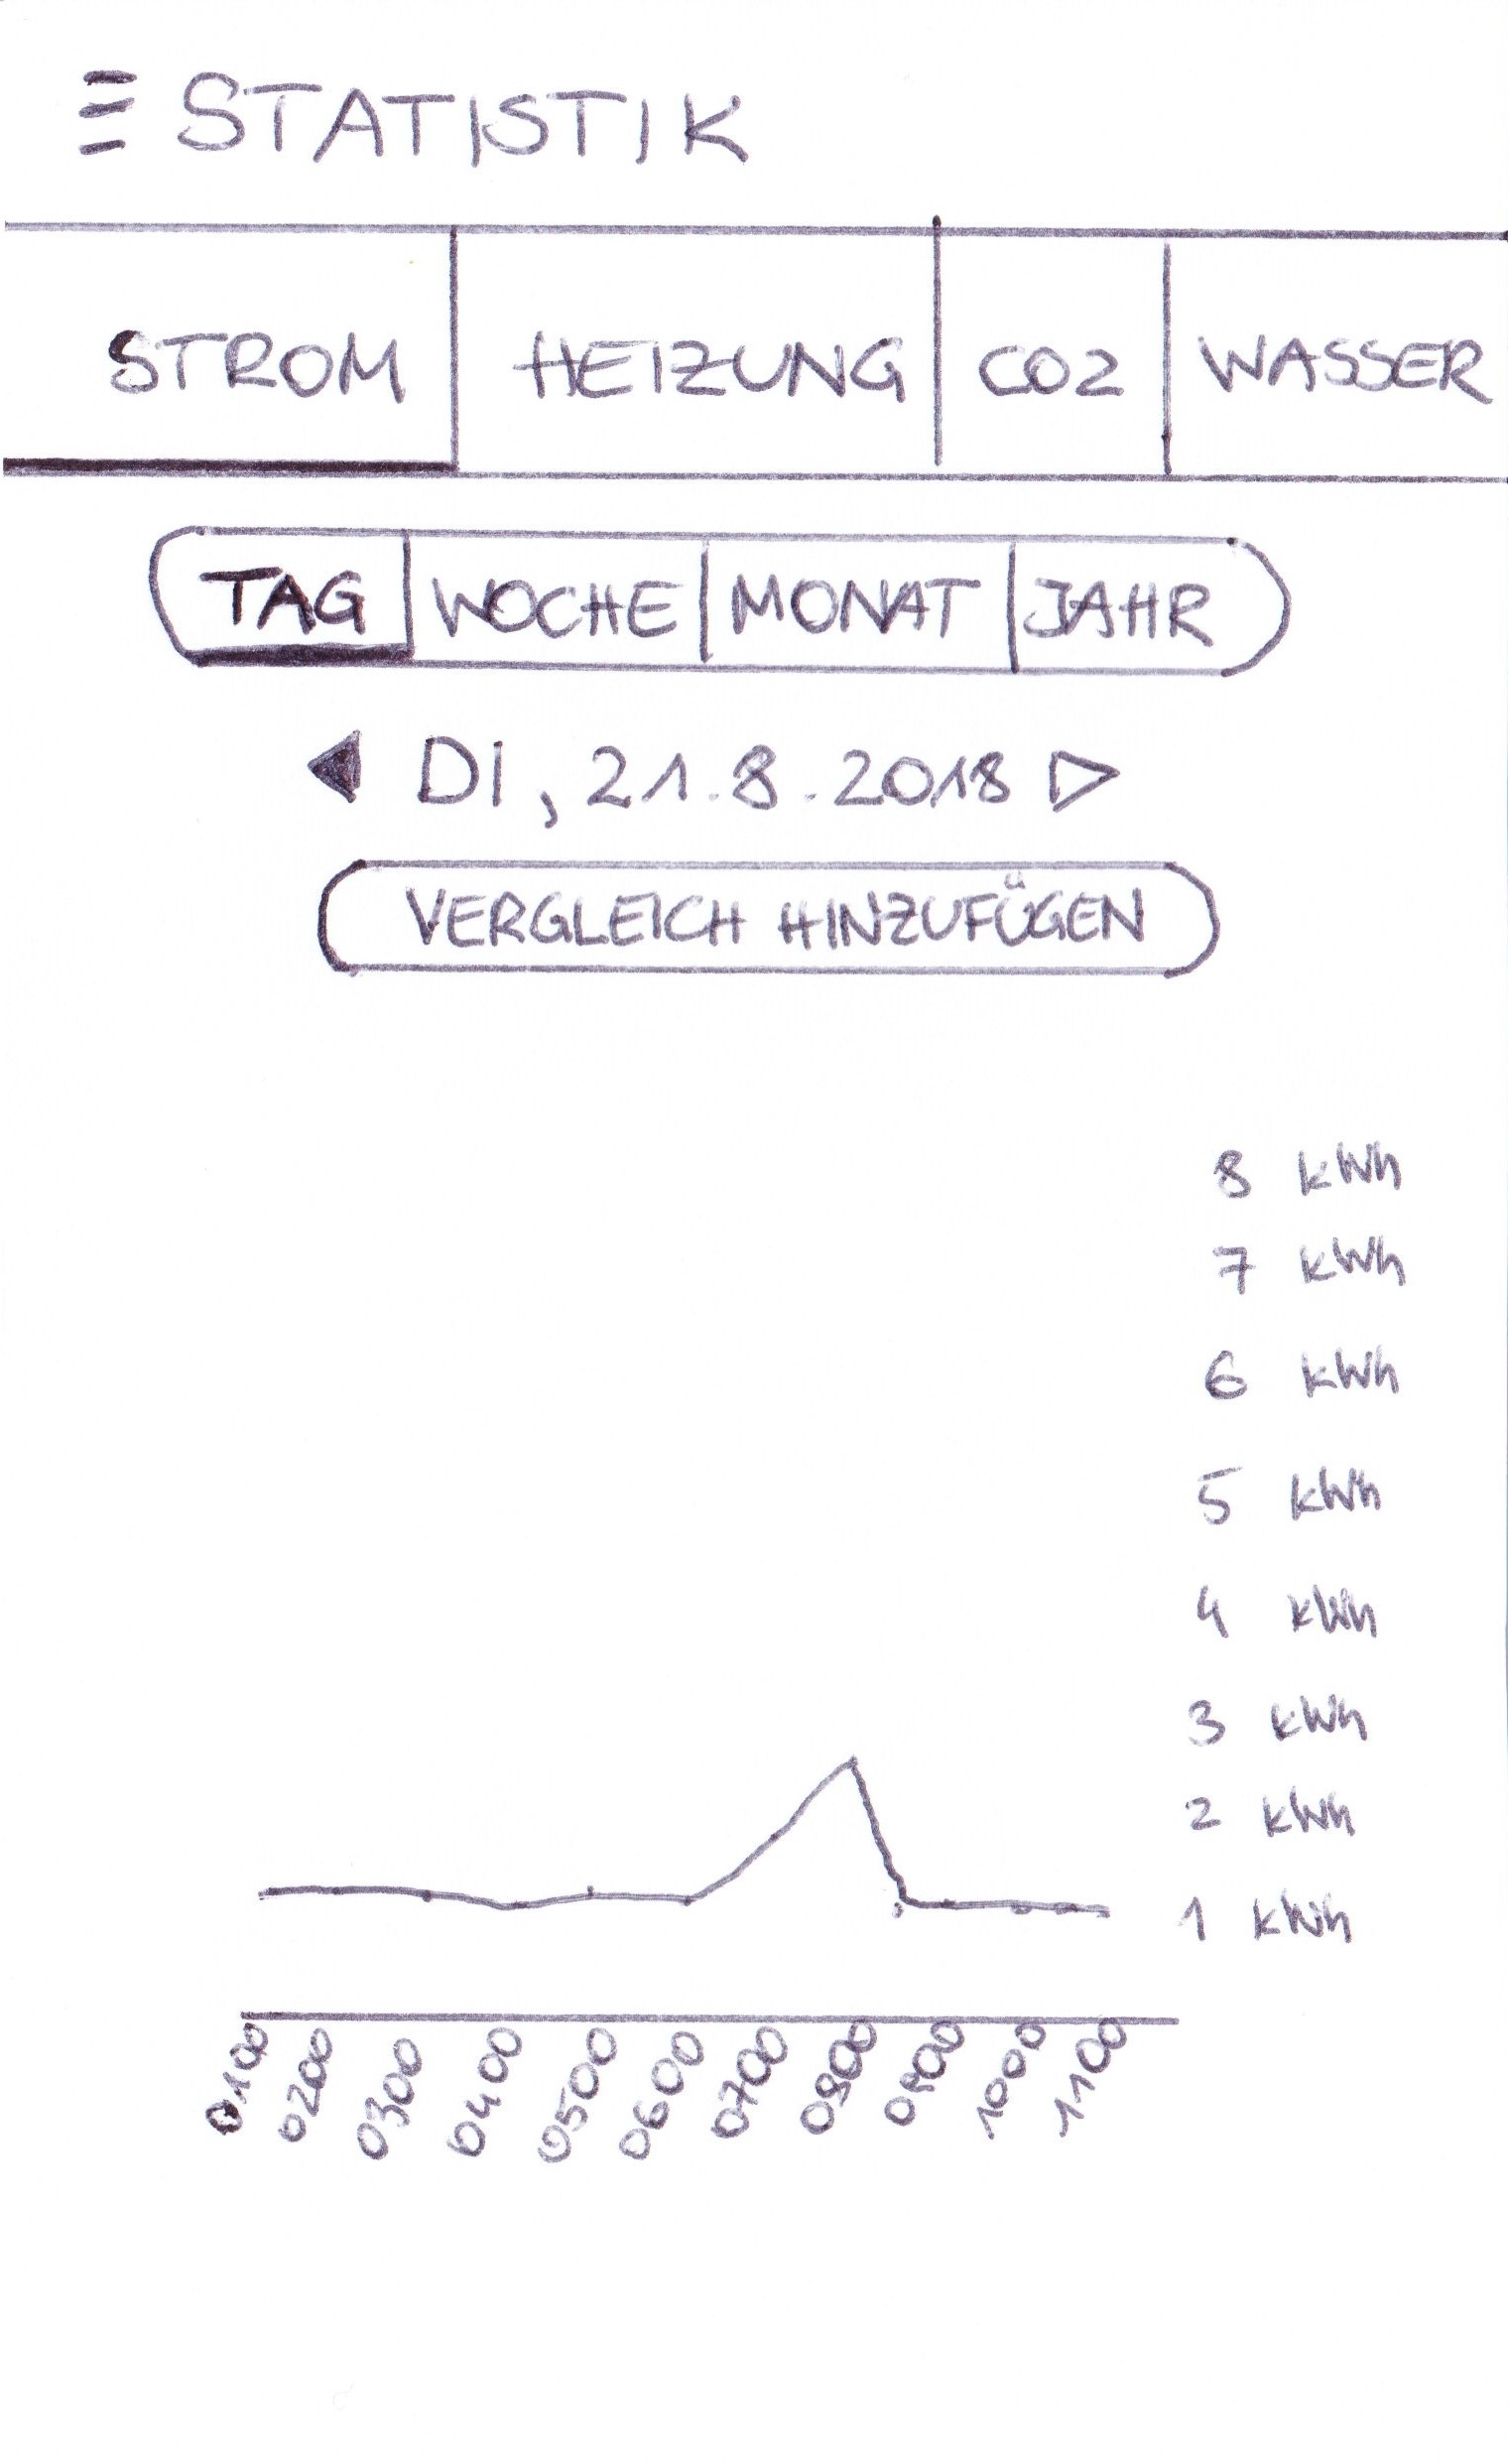
\includegraphics[width=\textwidth]{screens/Statistik_1234}
		\subcaption{Professional and Hedonist}
		\label{fig:statistik:professional}
	\end{subfigure}
	\begin{subfigure}[b]{0.24\columnwidth}
		\centering
		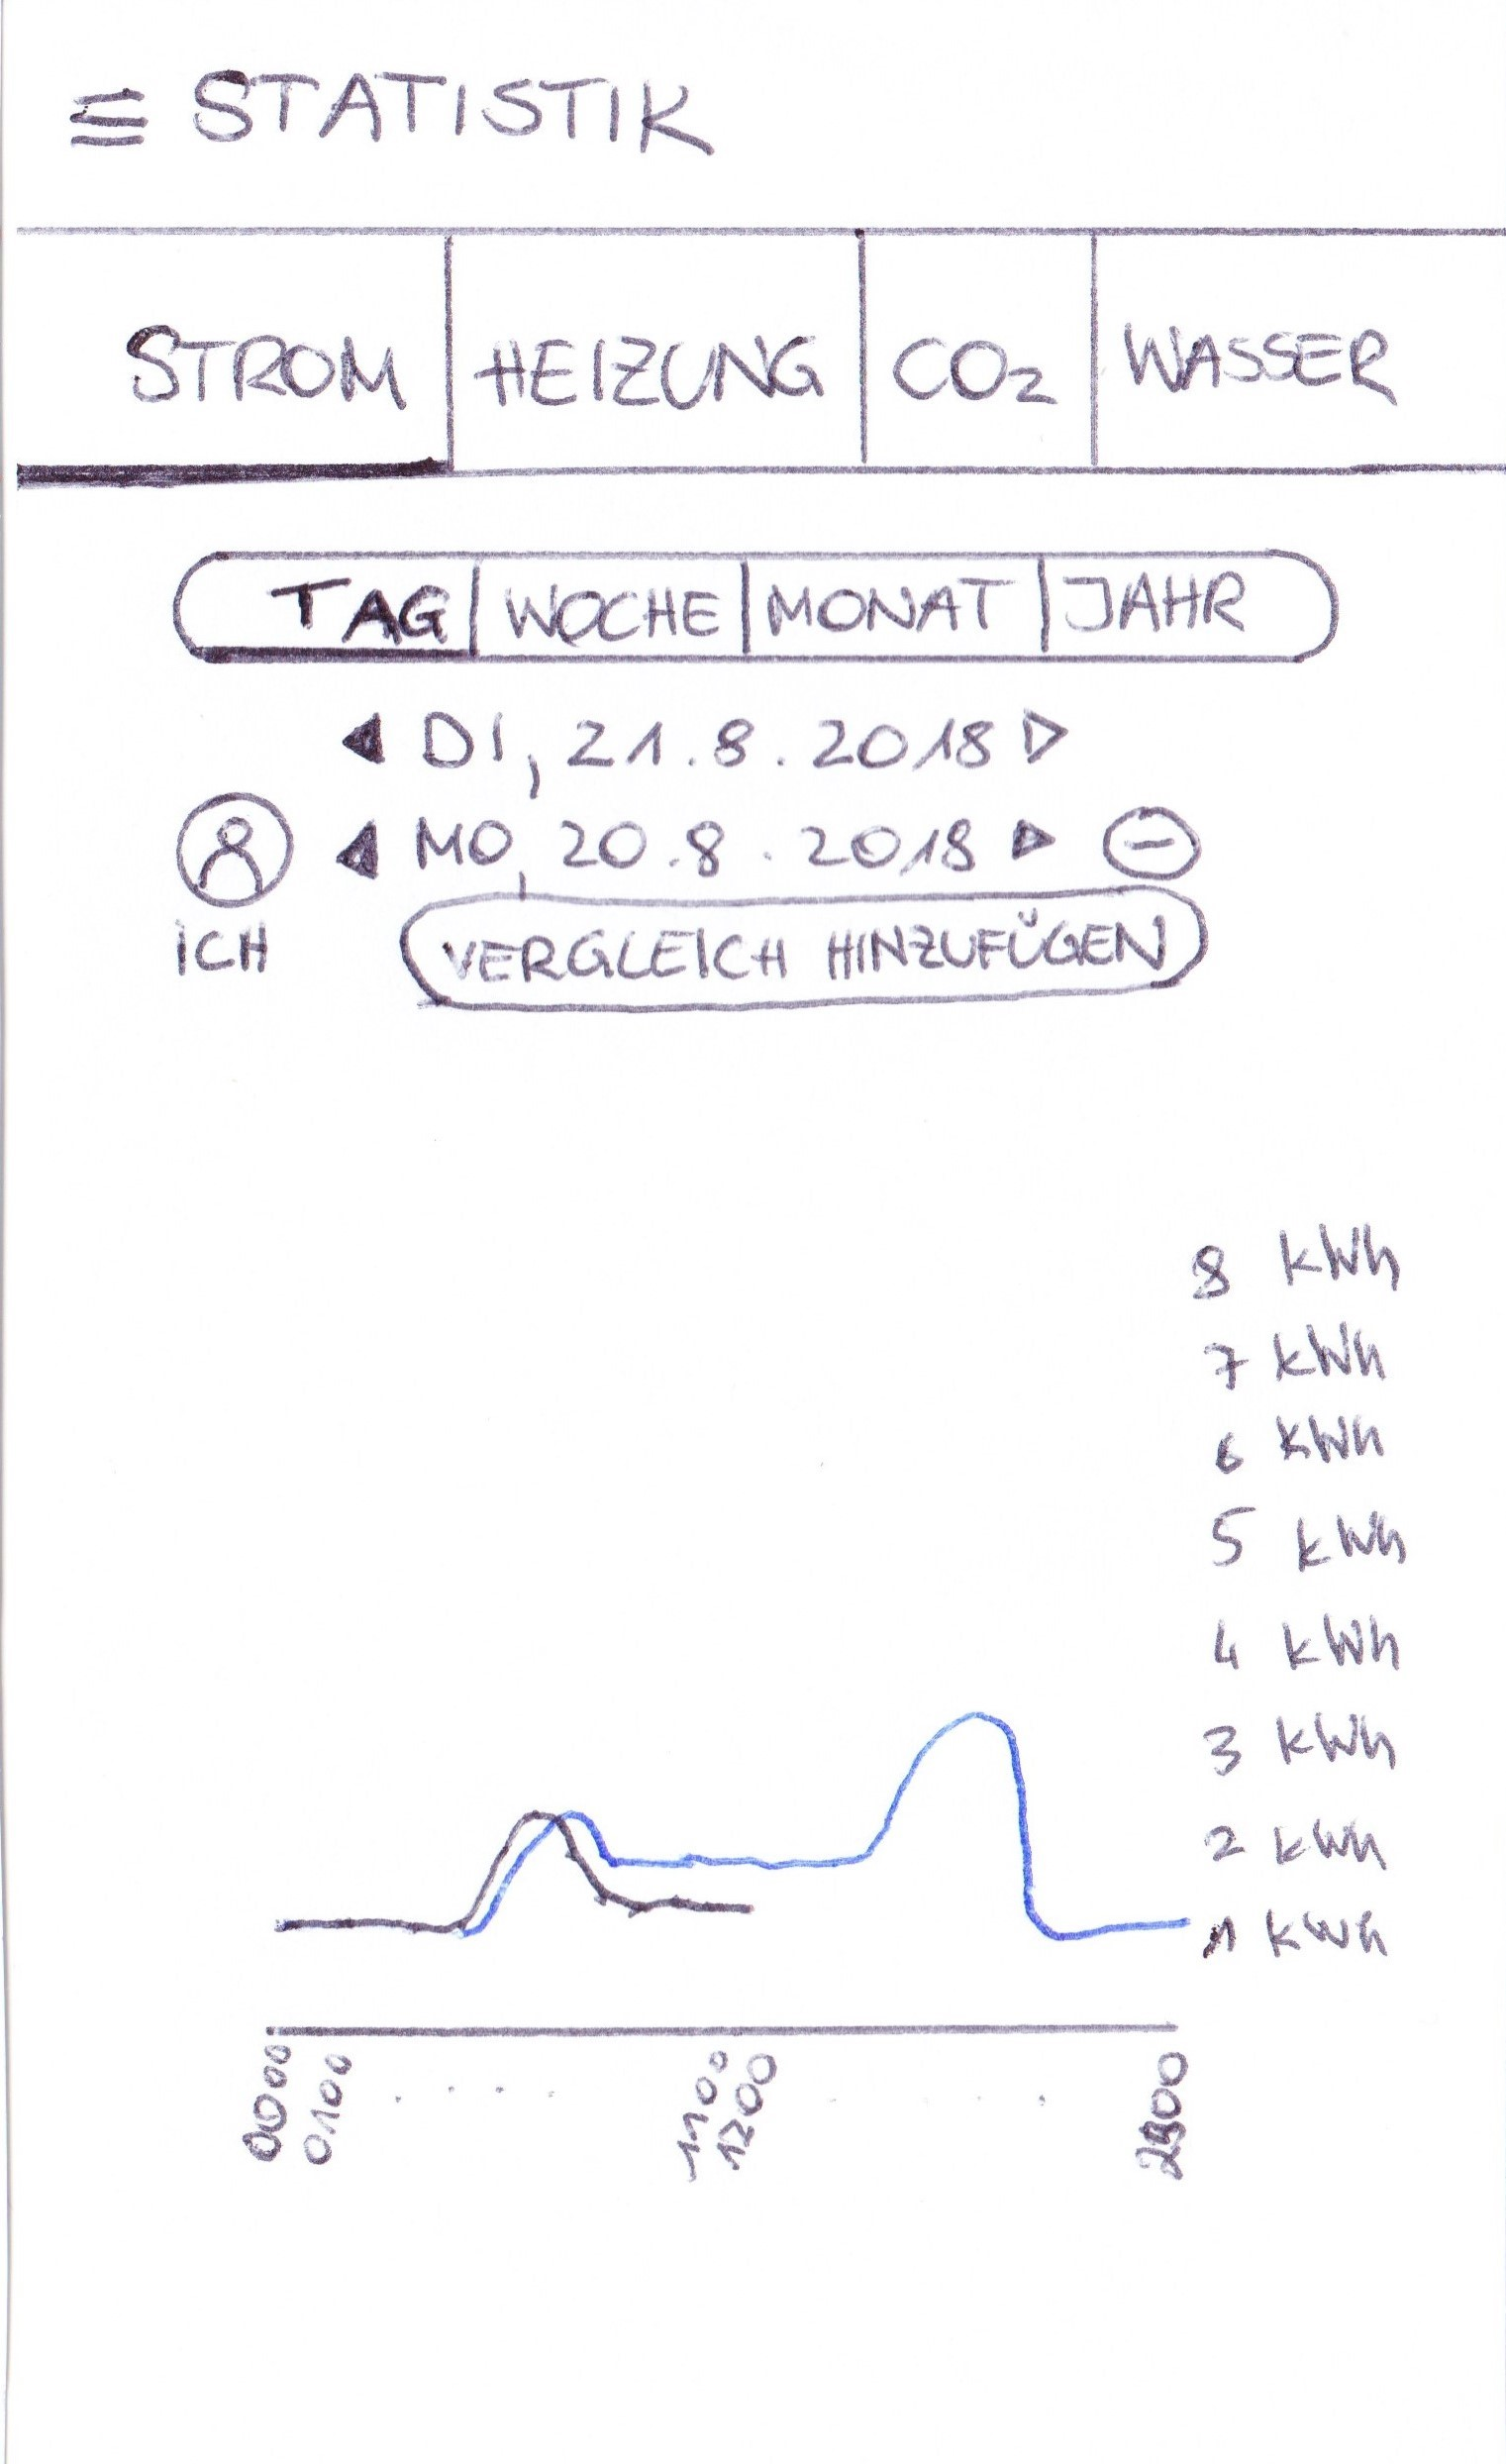
\includegraphics[width=\textwidth]{screens/Statistik_Vergleich}
		\subcaption{Optimizer and Indifferent}
		\label{fig:statistik:optimizer}
	\end{subfigure}
	\caption{The proposed screens for statistics}
	\label{fig:statistik} % \label has to be placed AFTER \caption (or \subcaption) to produce correct cross-references.
\end{figure}

\section{Equipment control}

\begin{figure}[h]
	\centering
	\begin{subfigure}[b]{0.24\columnwidth}
		\centering
		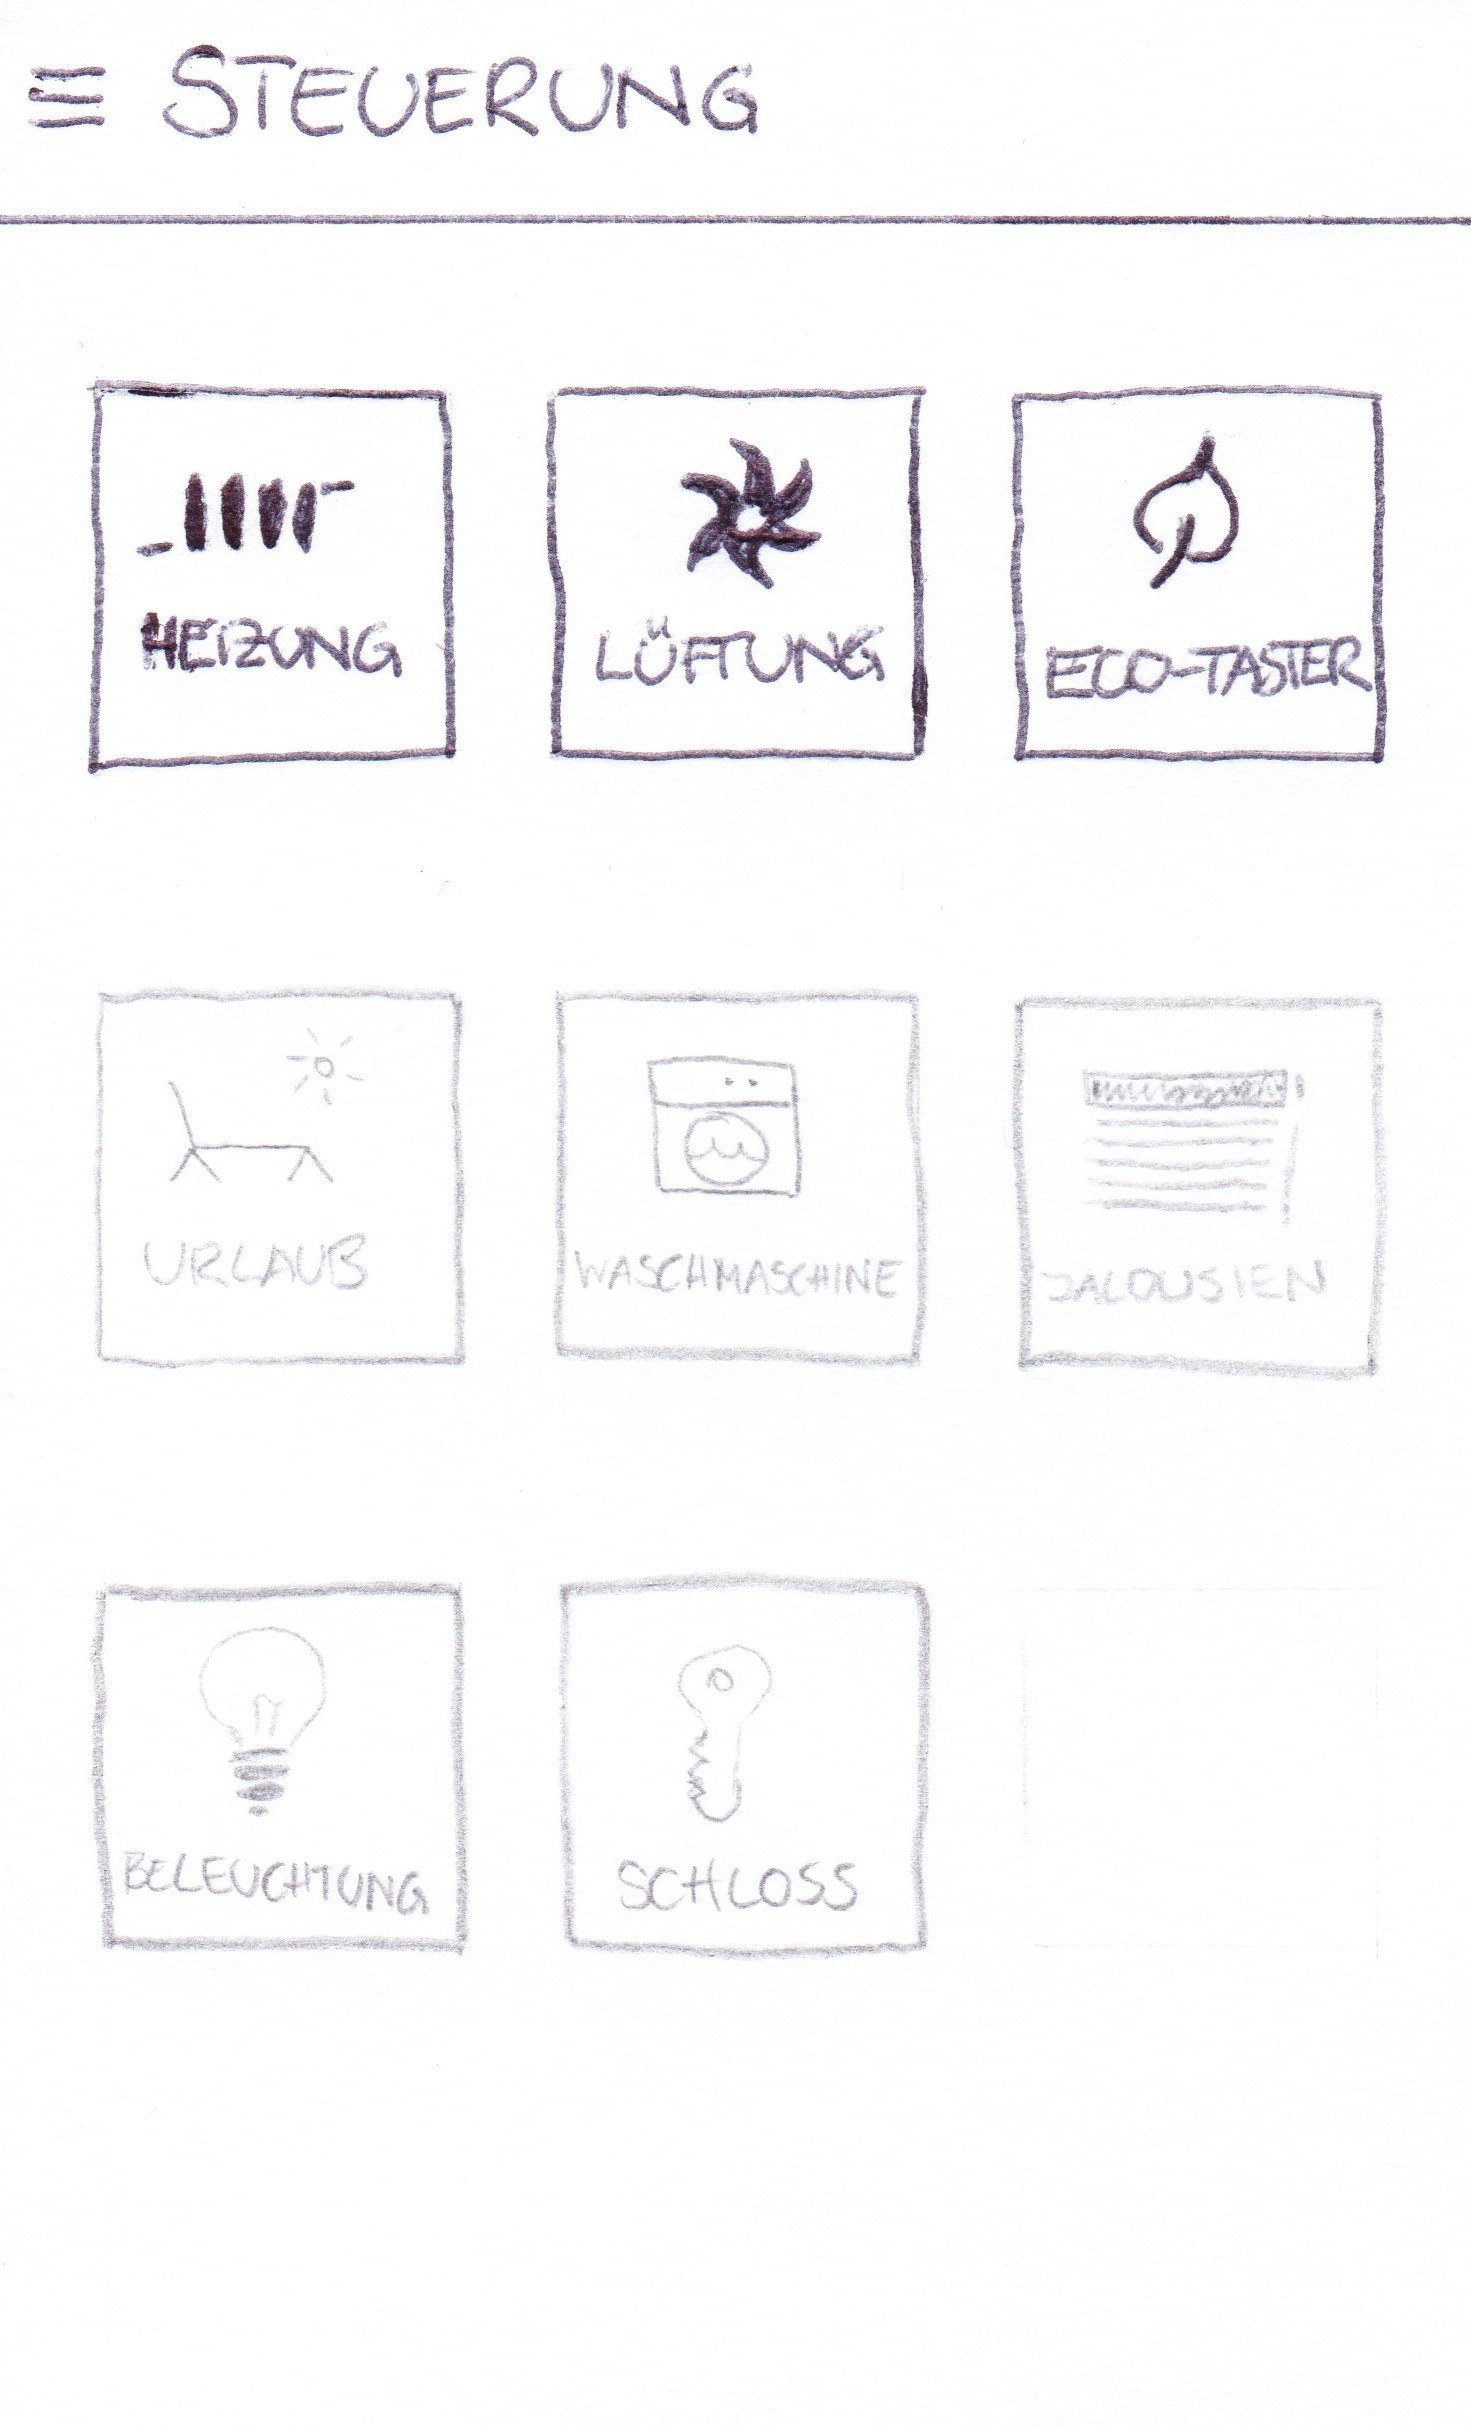
\includegraphics[width=\textwidth]{screens/Steuerung_1234}
		\subcaption{Professional and Hedonist}
		\label{fig:statistik:professional}
	\end{subfigure}
	\begin{subfigure}[b]{0.24\columnwidth}
		\centering
		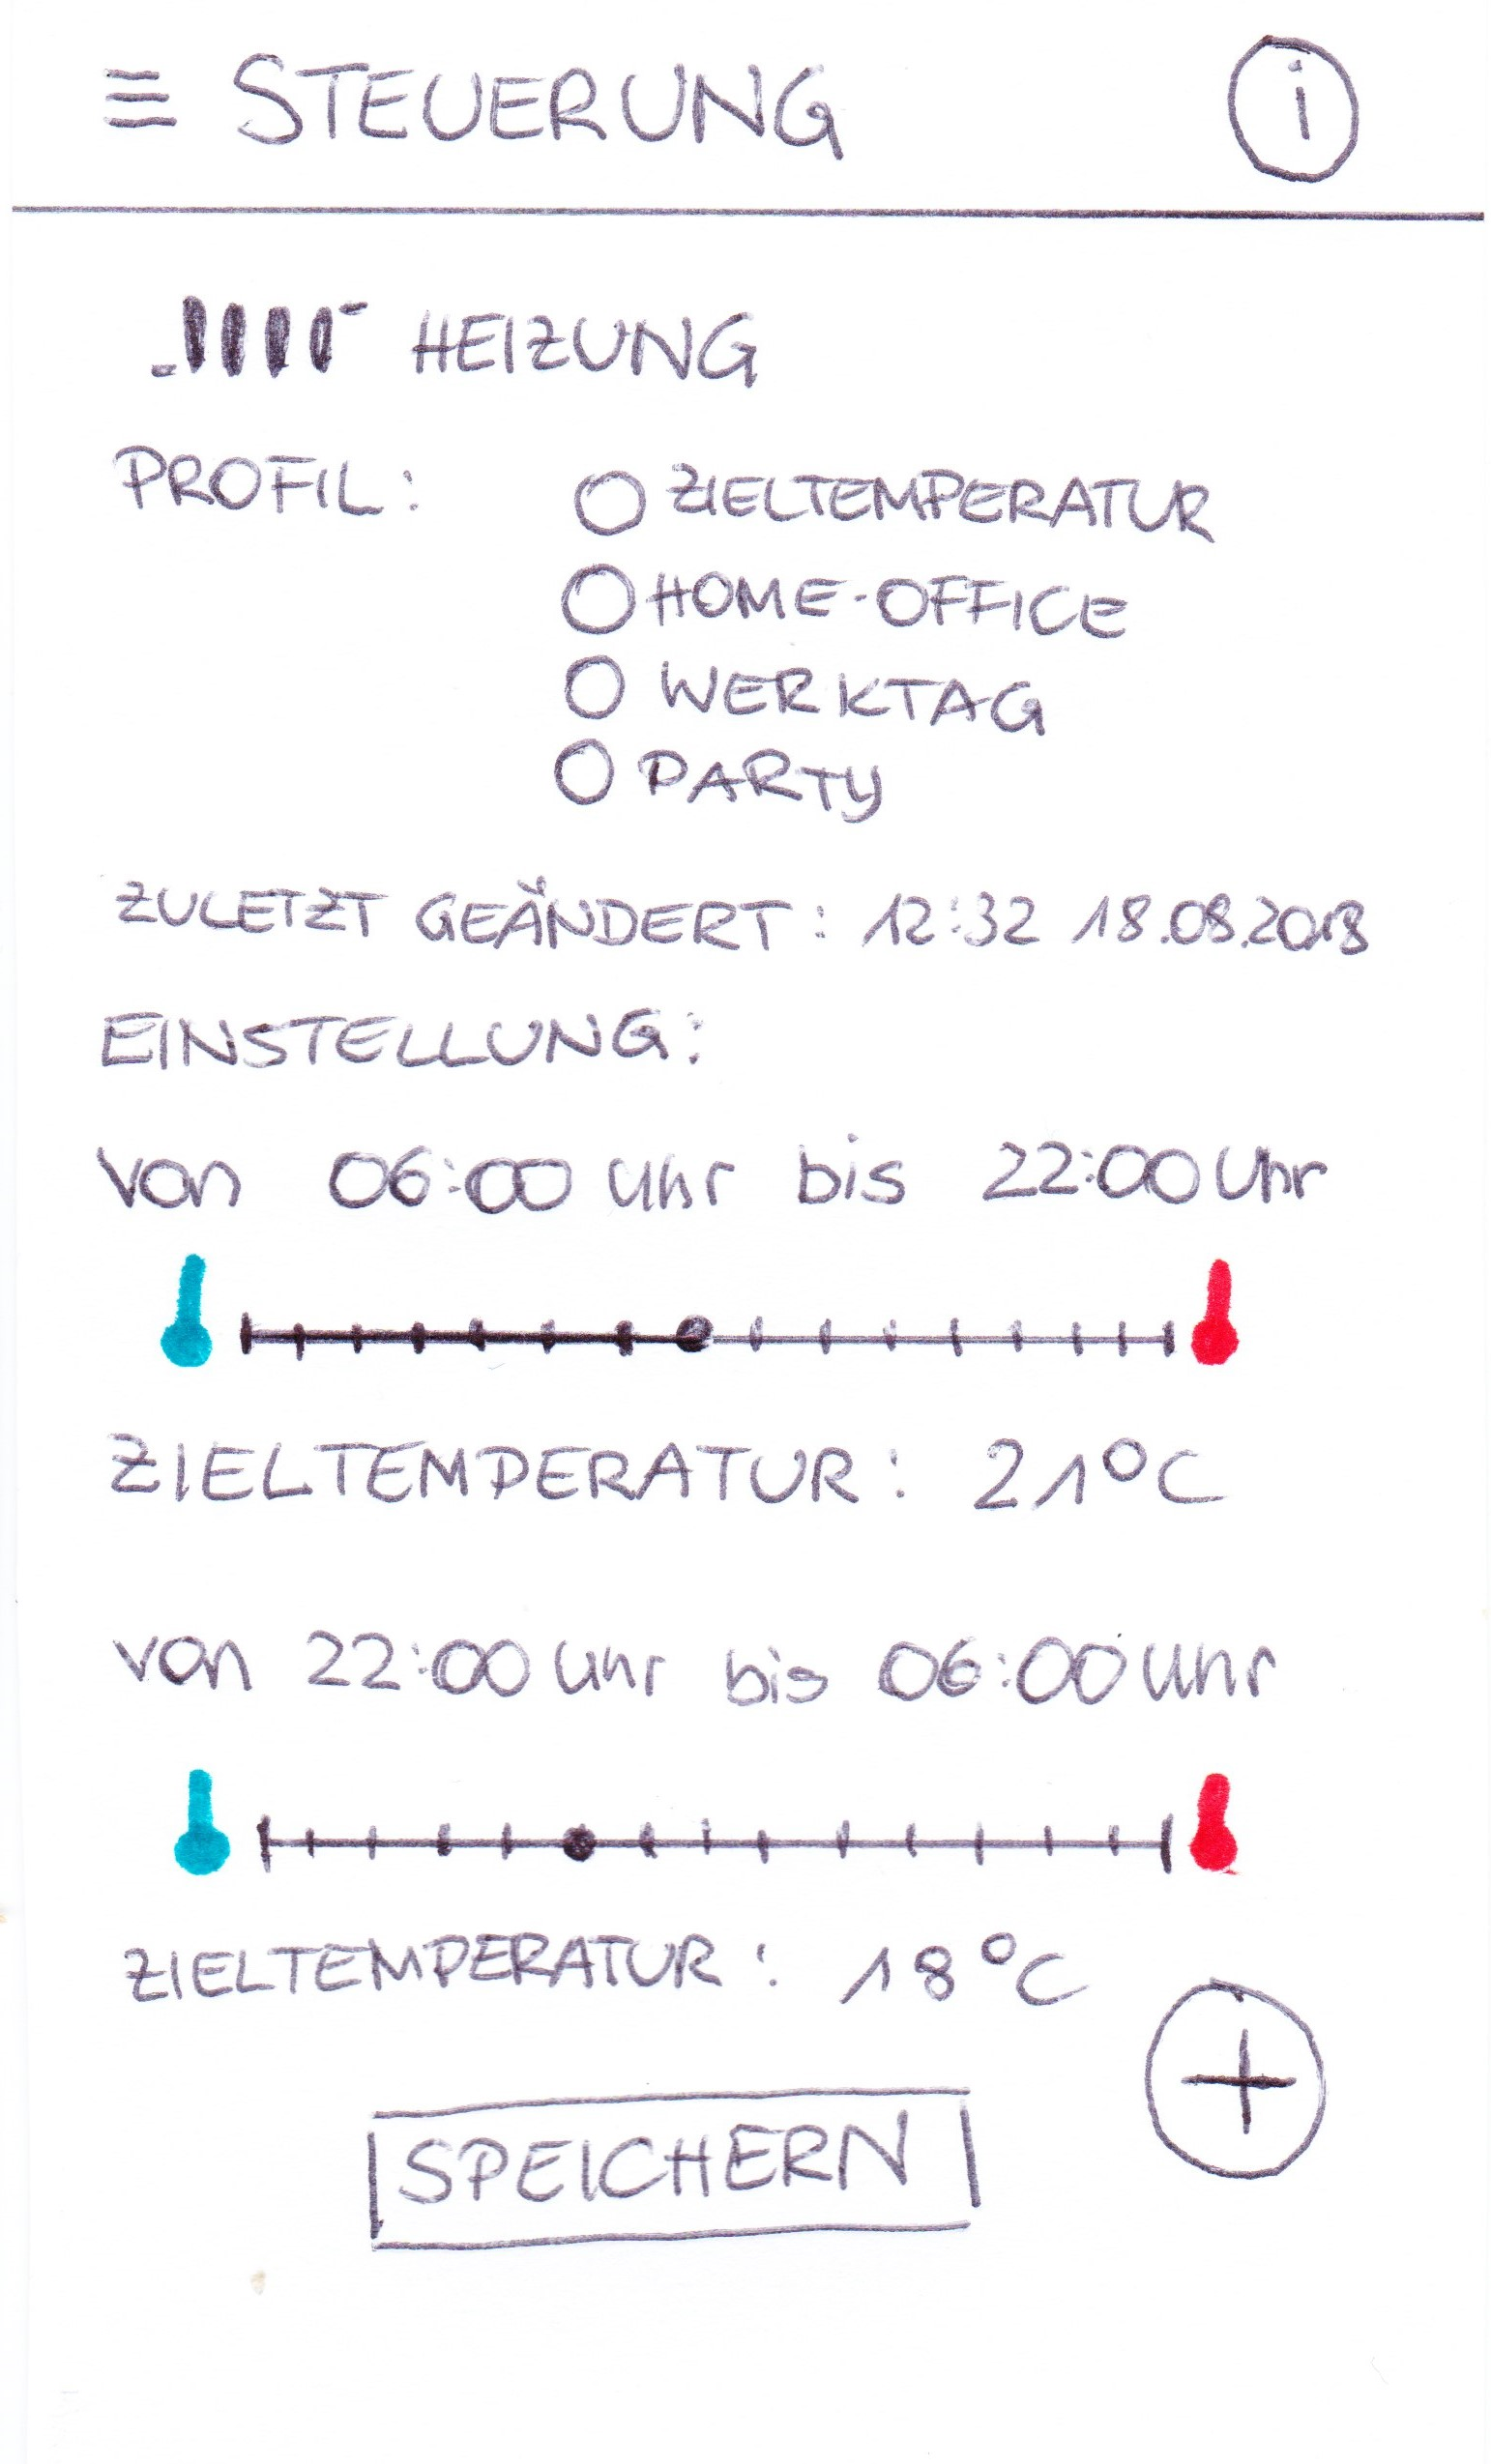
\includegraphics[width=\textwidth]{screens/Steuerung_Heizung}
		\subcaption{Optimizer and Indifferent}
		\label{fig:statistik:optimizer}
	\end{subfigure}
	\caption{The proposed screens for equipment control}
	\label{fig:statistik} % \label has to be placed AFTER \caption (or \subcaption) to produce correct cross-references.
\end{figure}

\section{Comparison of Savings}

\begin{figure}[h]
	\centering
	\begin{subfigure}[b]{0.24\columnwidth}
		\centering
		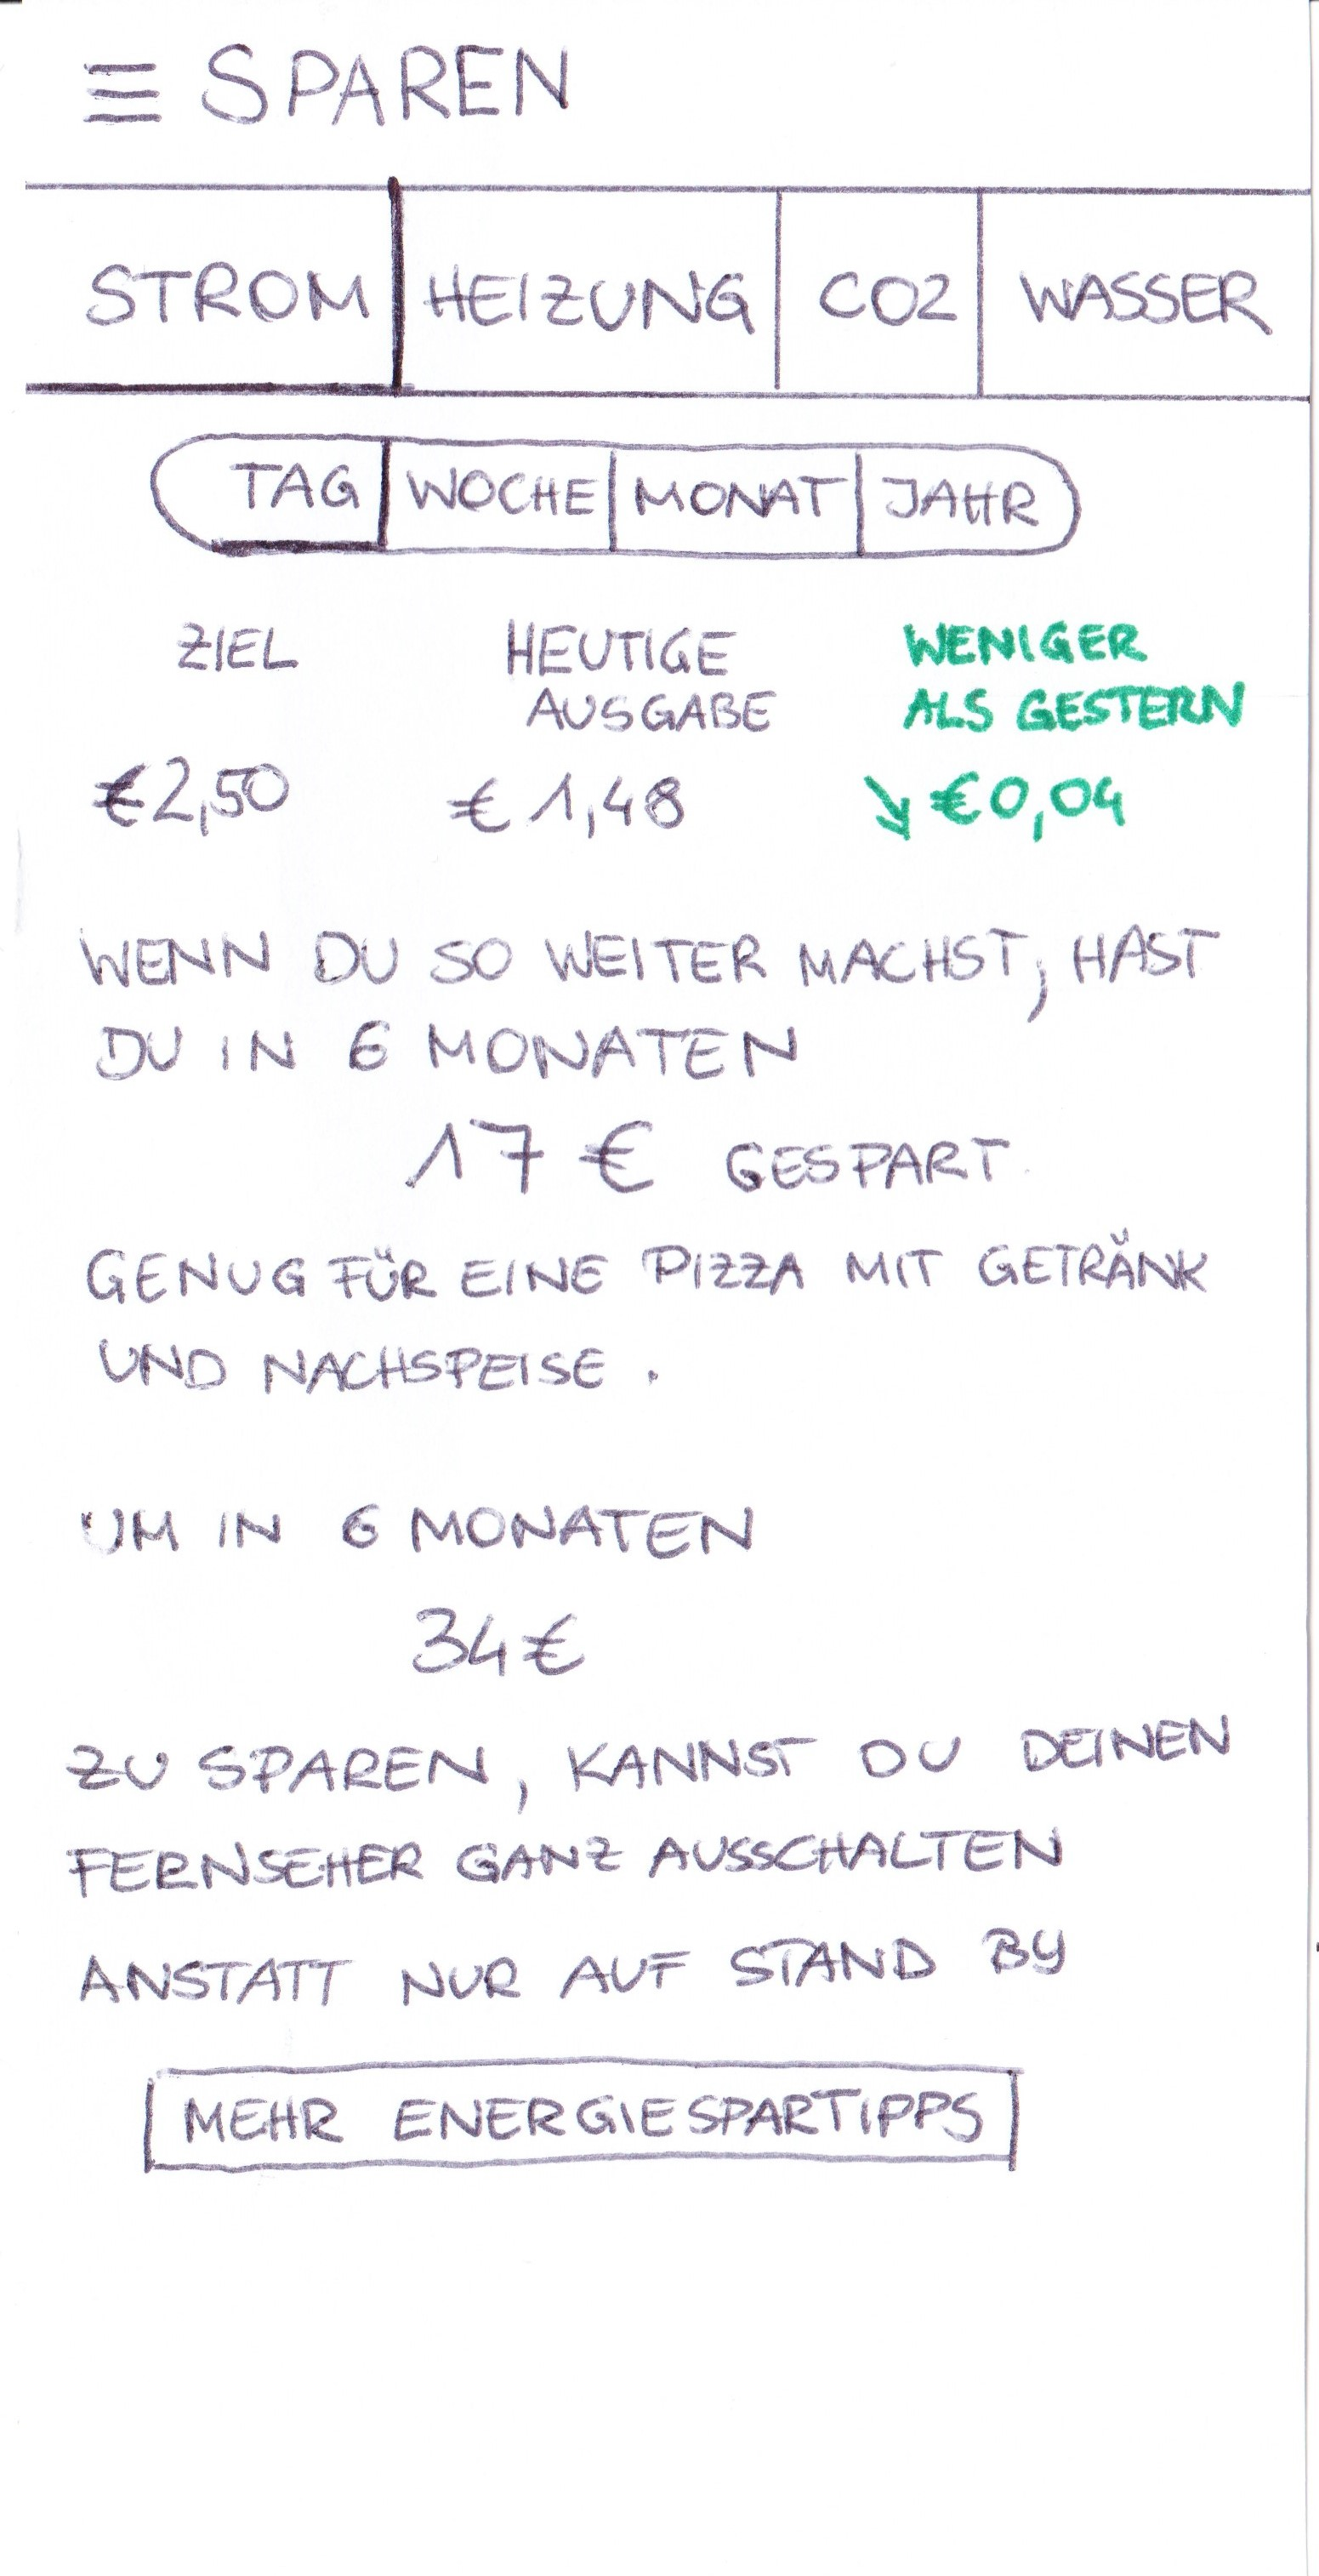
\includegraphics[width=\textwidth]{screens/Sparen_1}
		\subcaption{Professional}
		\label{fig:sparen:professional}
	\end{subfigure}
	\begin{subfigure}[b]{0.24\columnwidth}
		\centering
		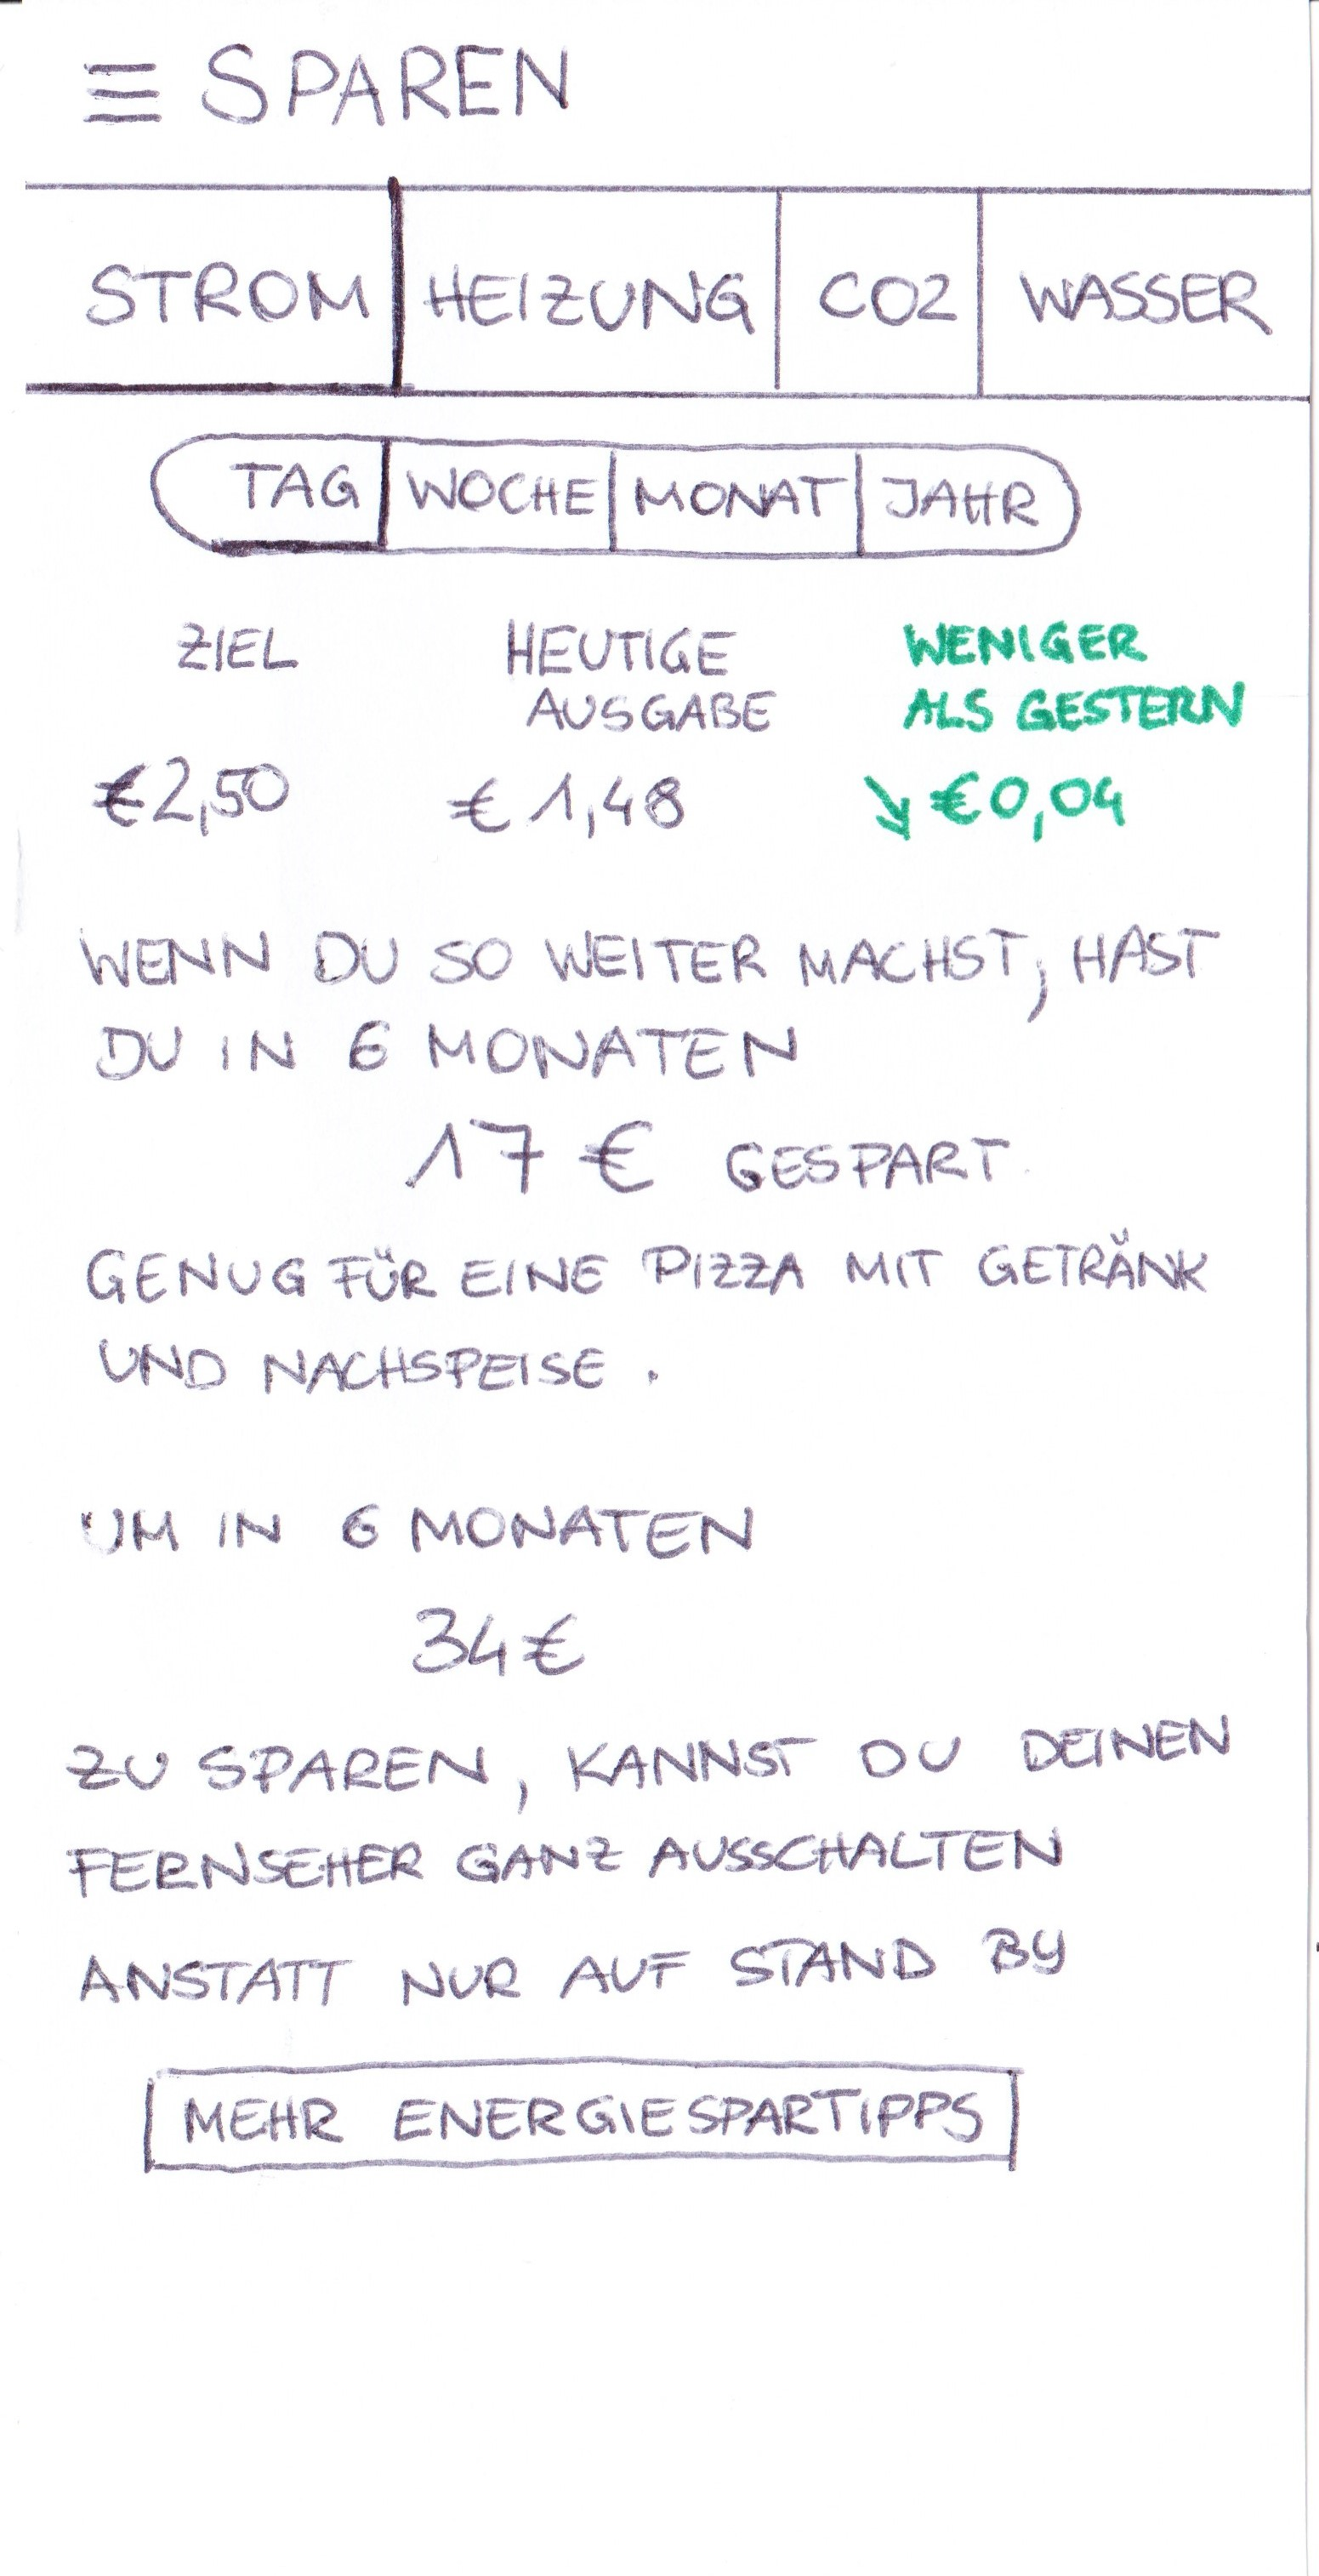
\includegraphics[width=\textwidth]{screens/Sparen_2}
		\subcaption{Optimizer}
		\label{fig:sparen:optimizer}
	\end{subfigure}
	\begin{subfigure}[b]{0.24\columnwidth}
		\centering
		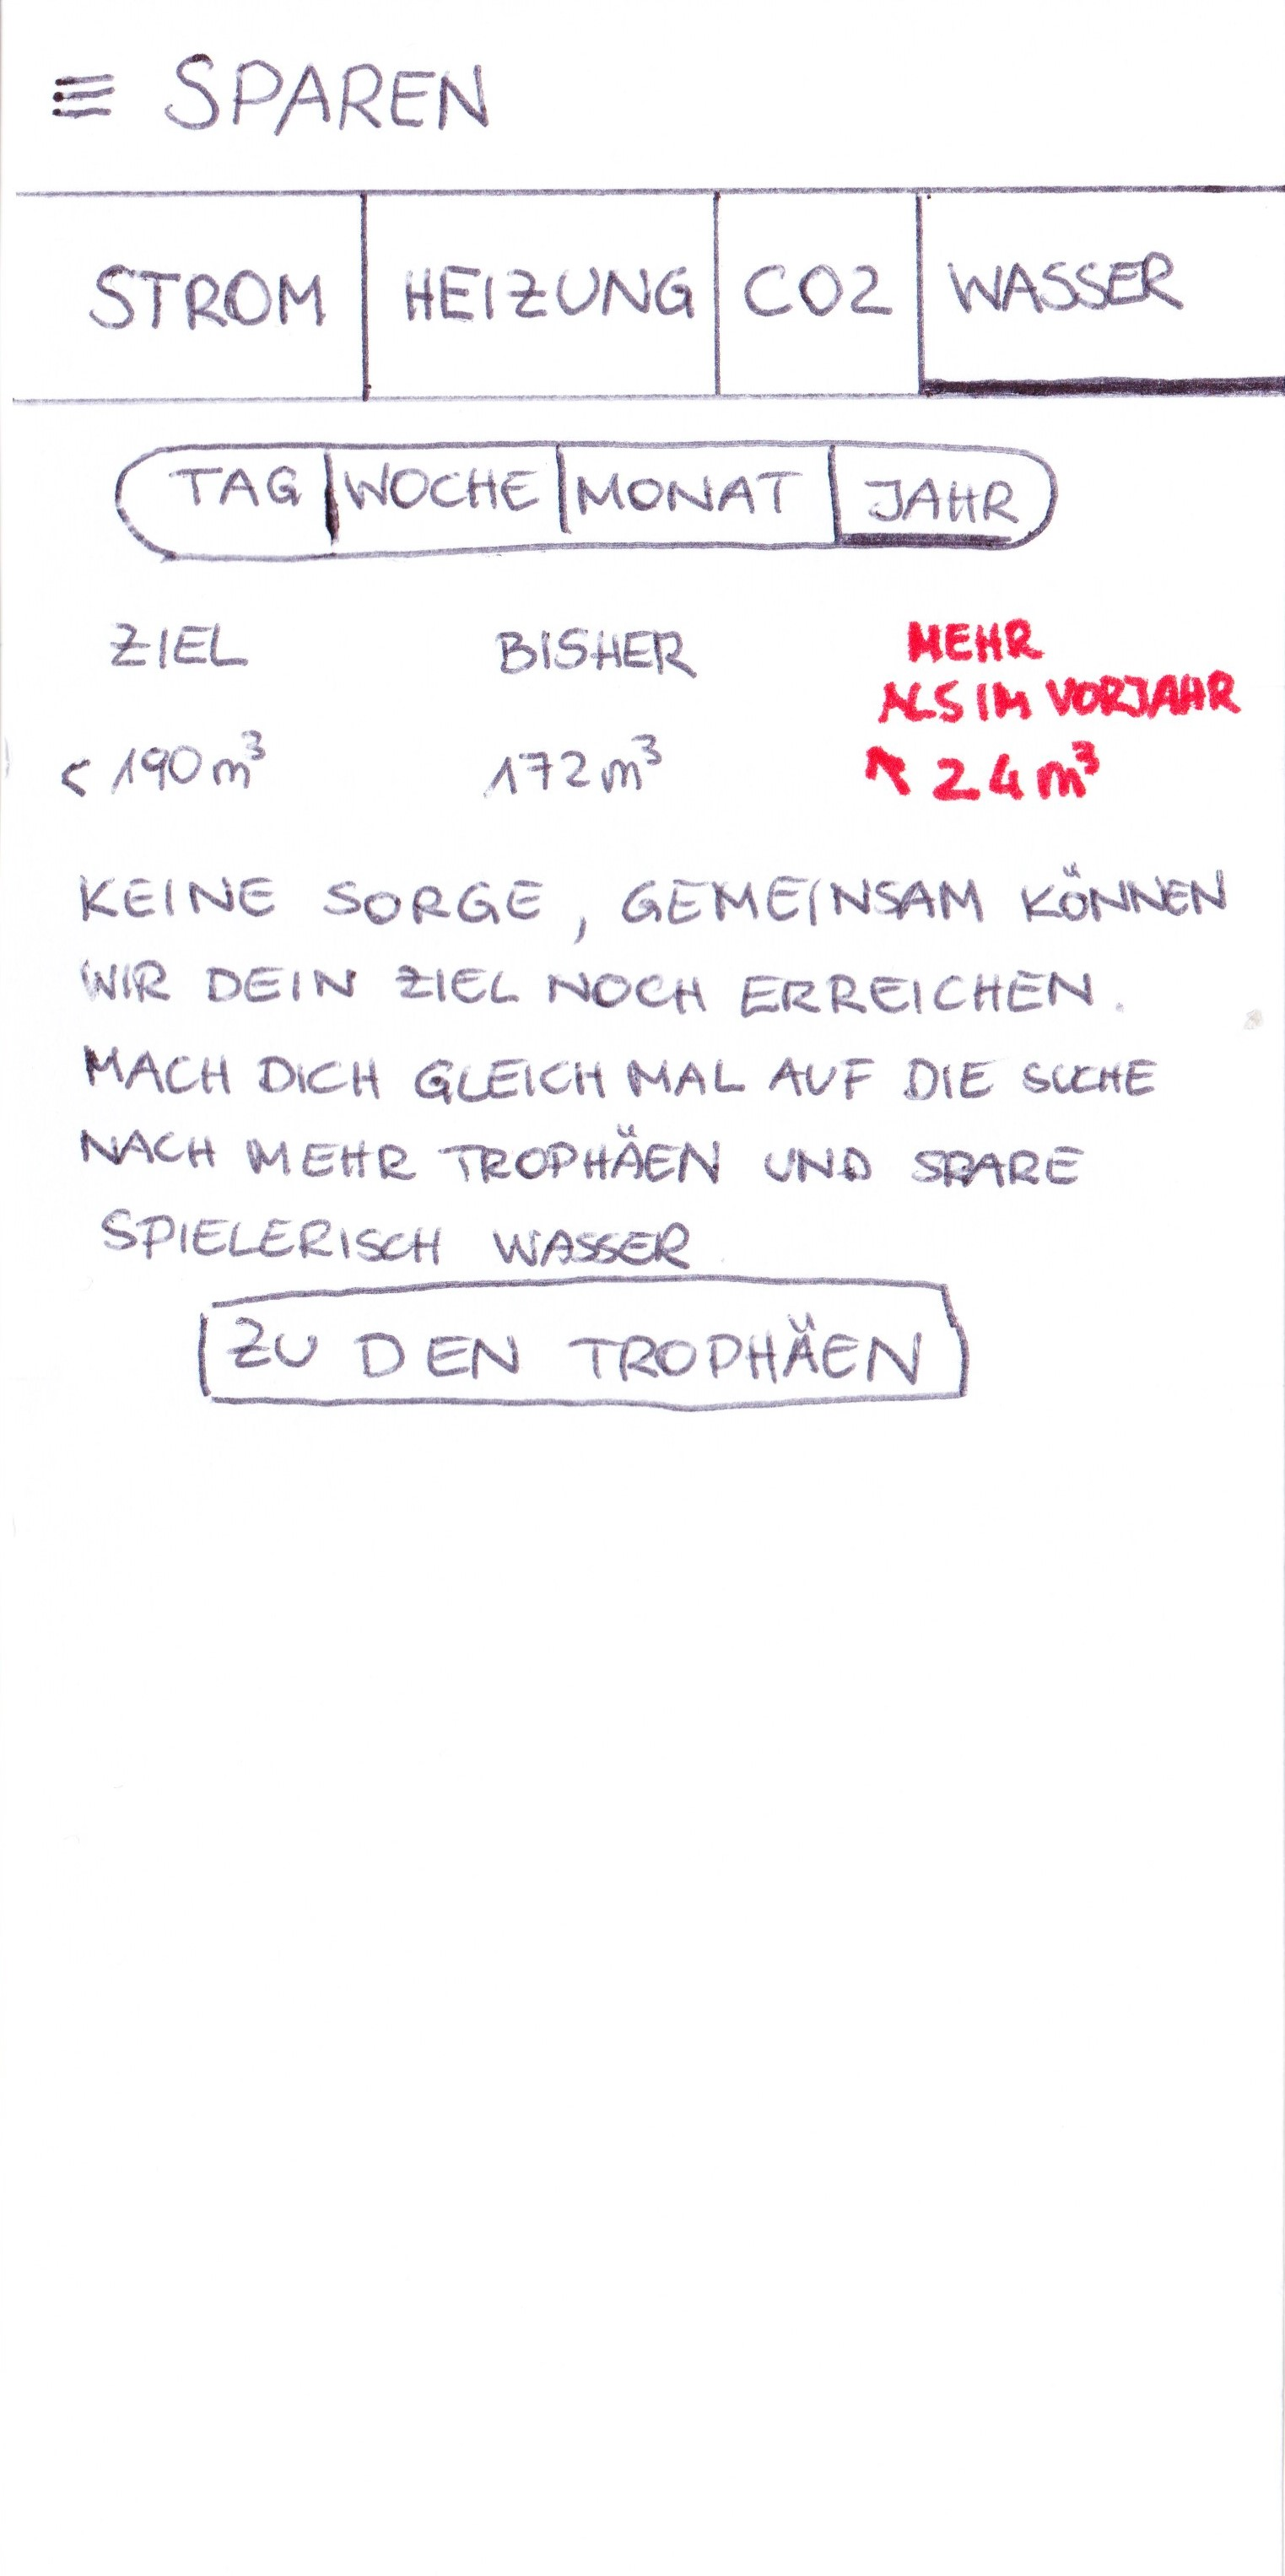
\includegraphics[width=\textwidth]{screens/Sparen_3}
		\subcaption{Indifferent}
		\label{fig:sparen:indifferent}
	\end{subfigure}
	\begin{subfigure}[b]{0.24\columnwidth}
		\centering
		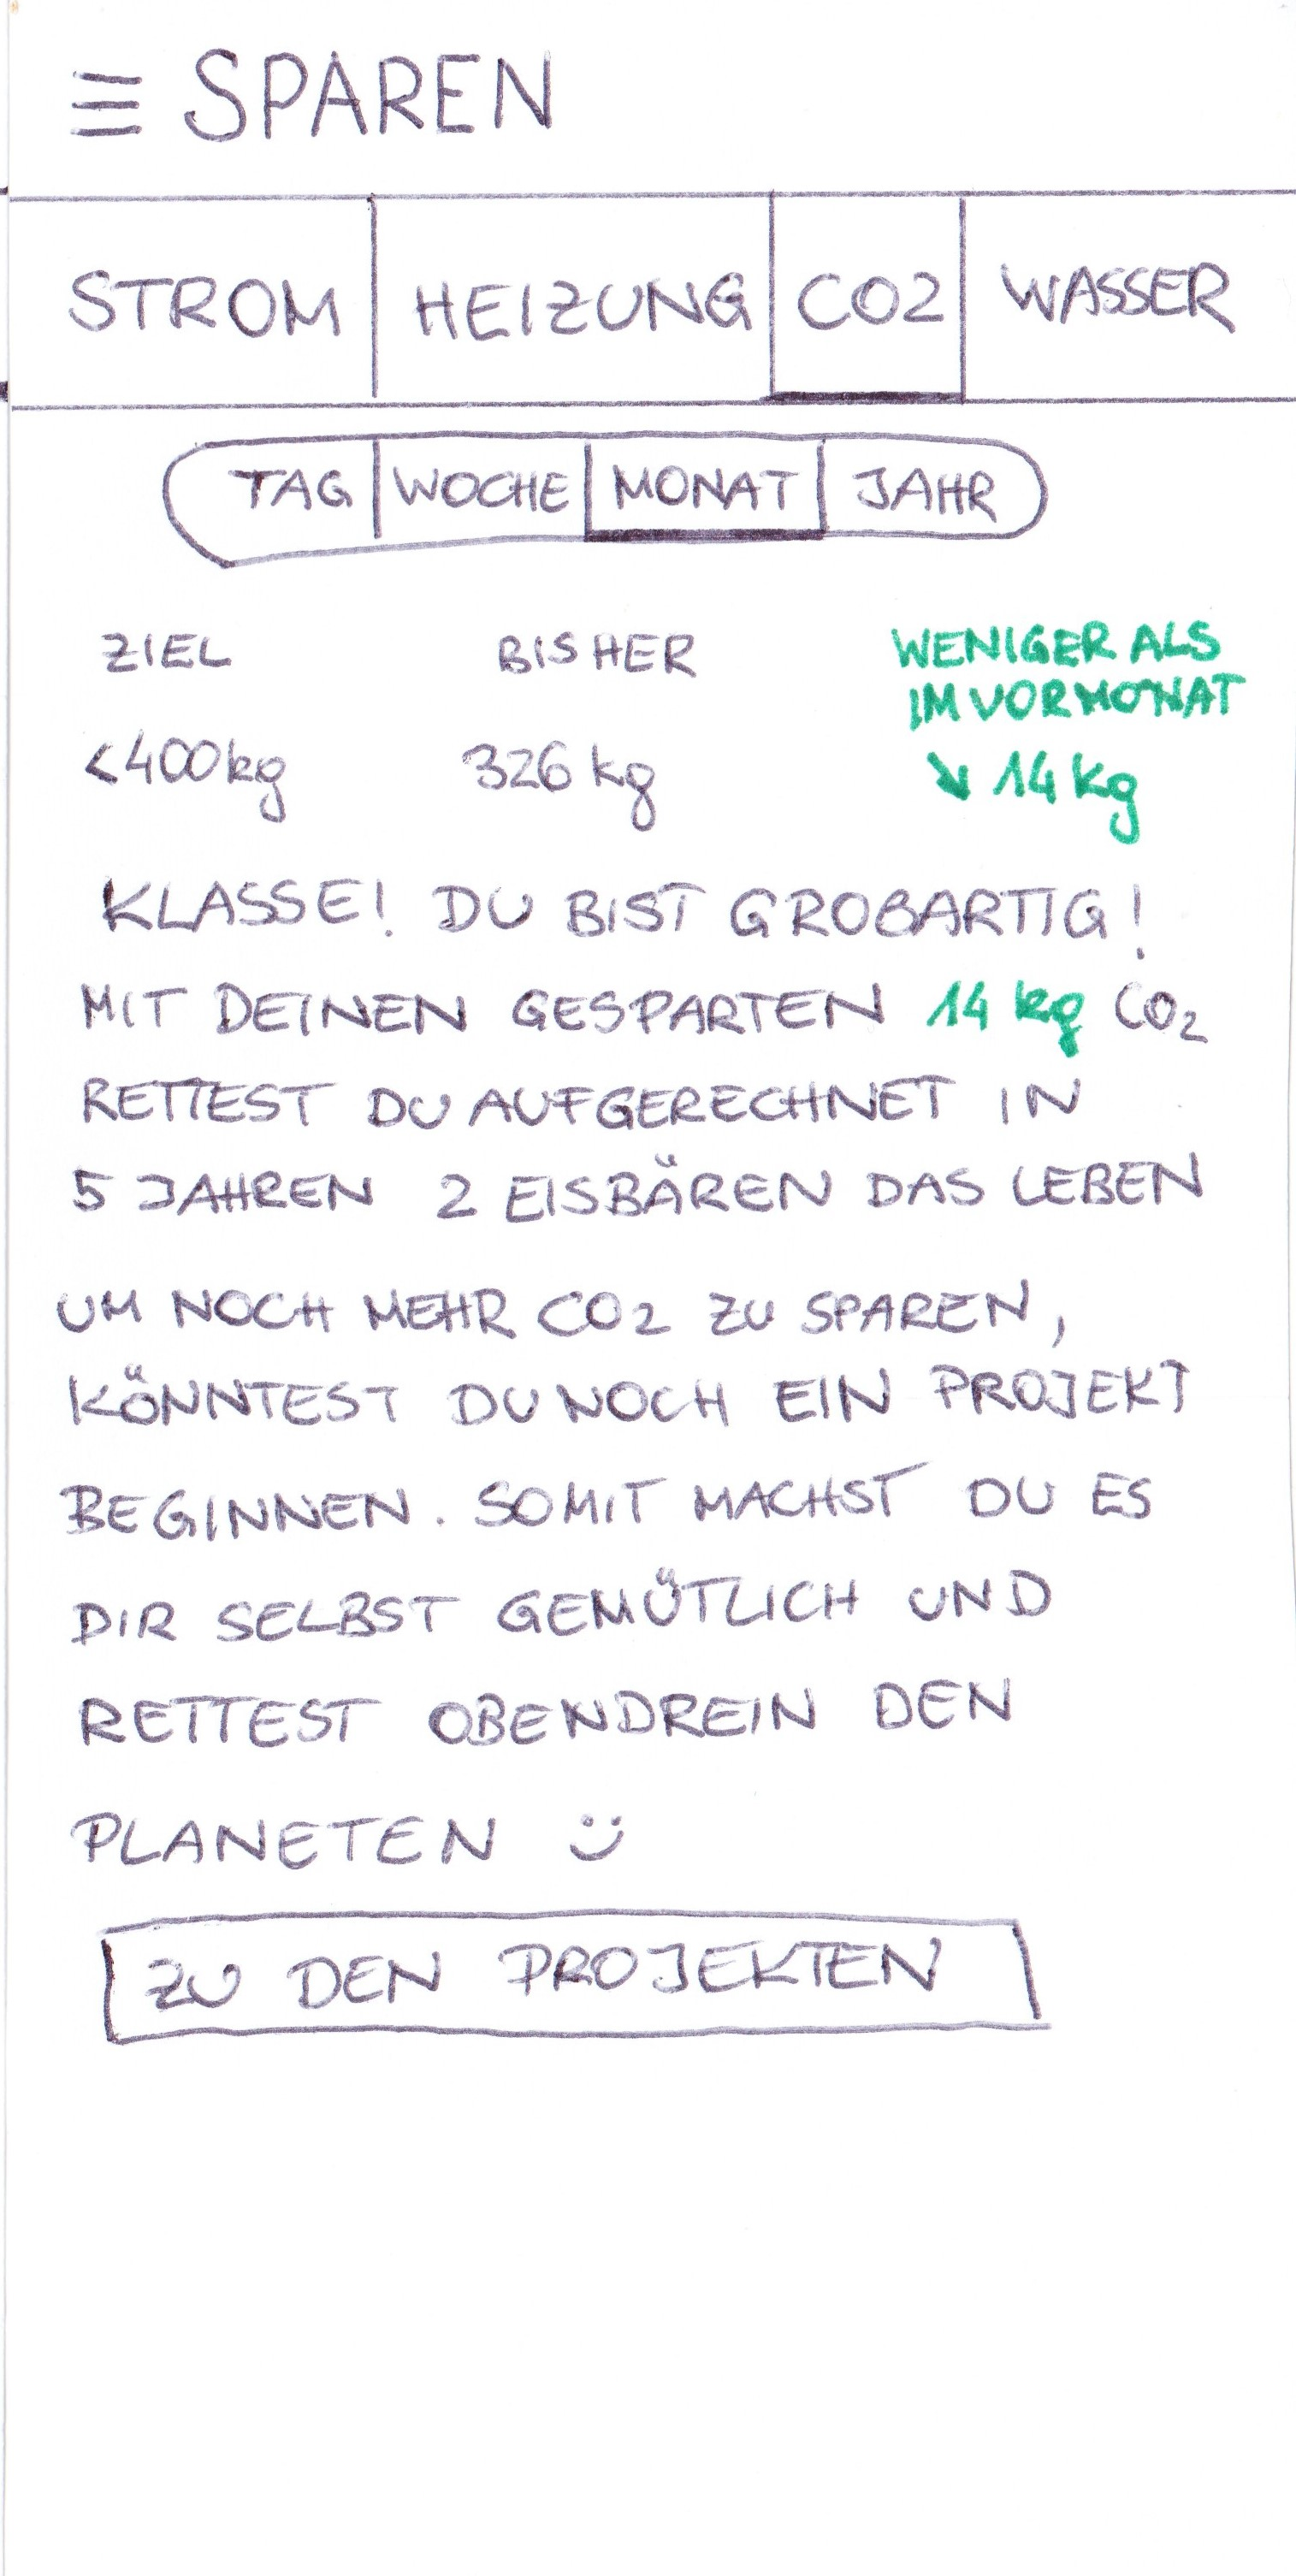
\includegraphics[width=\textwidth]{screens/Sparen_4}
		\subcaption{Hedonist}
		\label{fig:sparen:hedonist}
	\end{subfigure}
	\caption{The paper prototype screen for saving}
	\label{fig:sparen} % \label has to be placed AFTER \caption (or \subcaption) to produce correct cross-references.
\end{figure}

\section{Energy-Saving Tips}

Hedonists prefer to do projects that save energy for them in the long run
Hedonists are comfort-oriented Do not present energy saving tips to Hedonists when they limit comfort
Professionals are interested in deeper information for saving tips
Professionals do not see gamification approaches as a motivation for saving energy tips
Optimizer want to know how much they can save by following an Energy-saving tip
Indifferents woul

\begin{figure}[h]
	\centering
	\begin{subfigure}[b]{0.24\columnwidth}
		\centering
		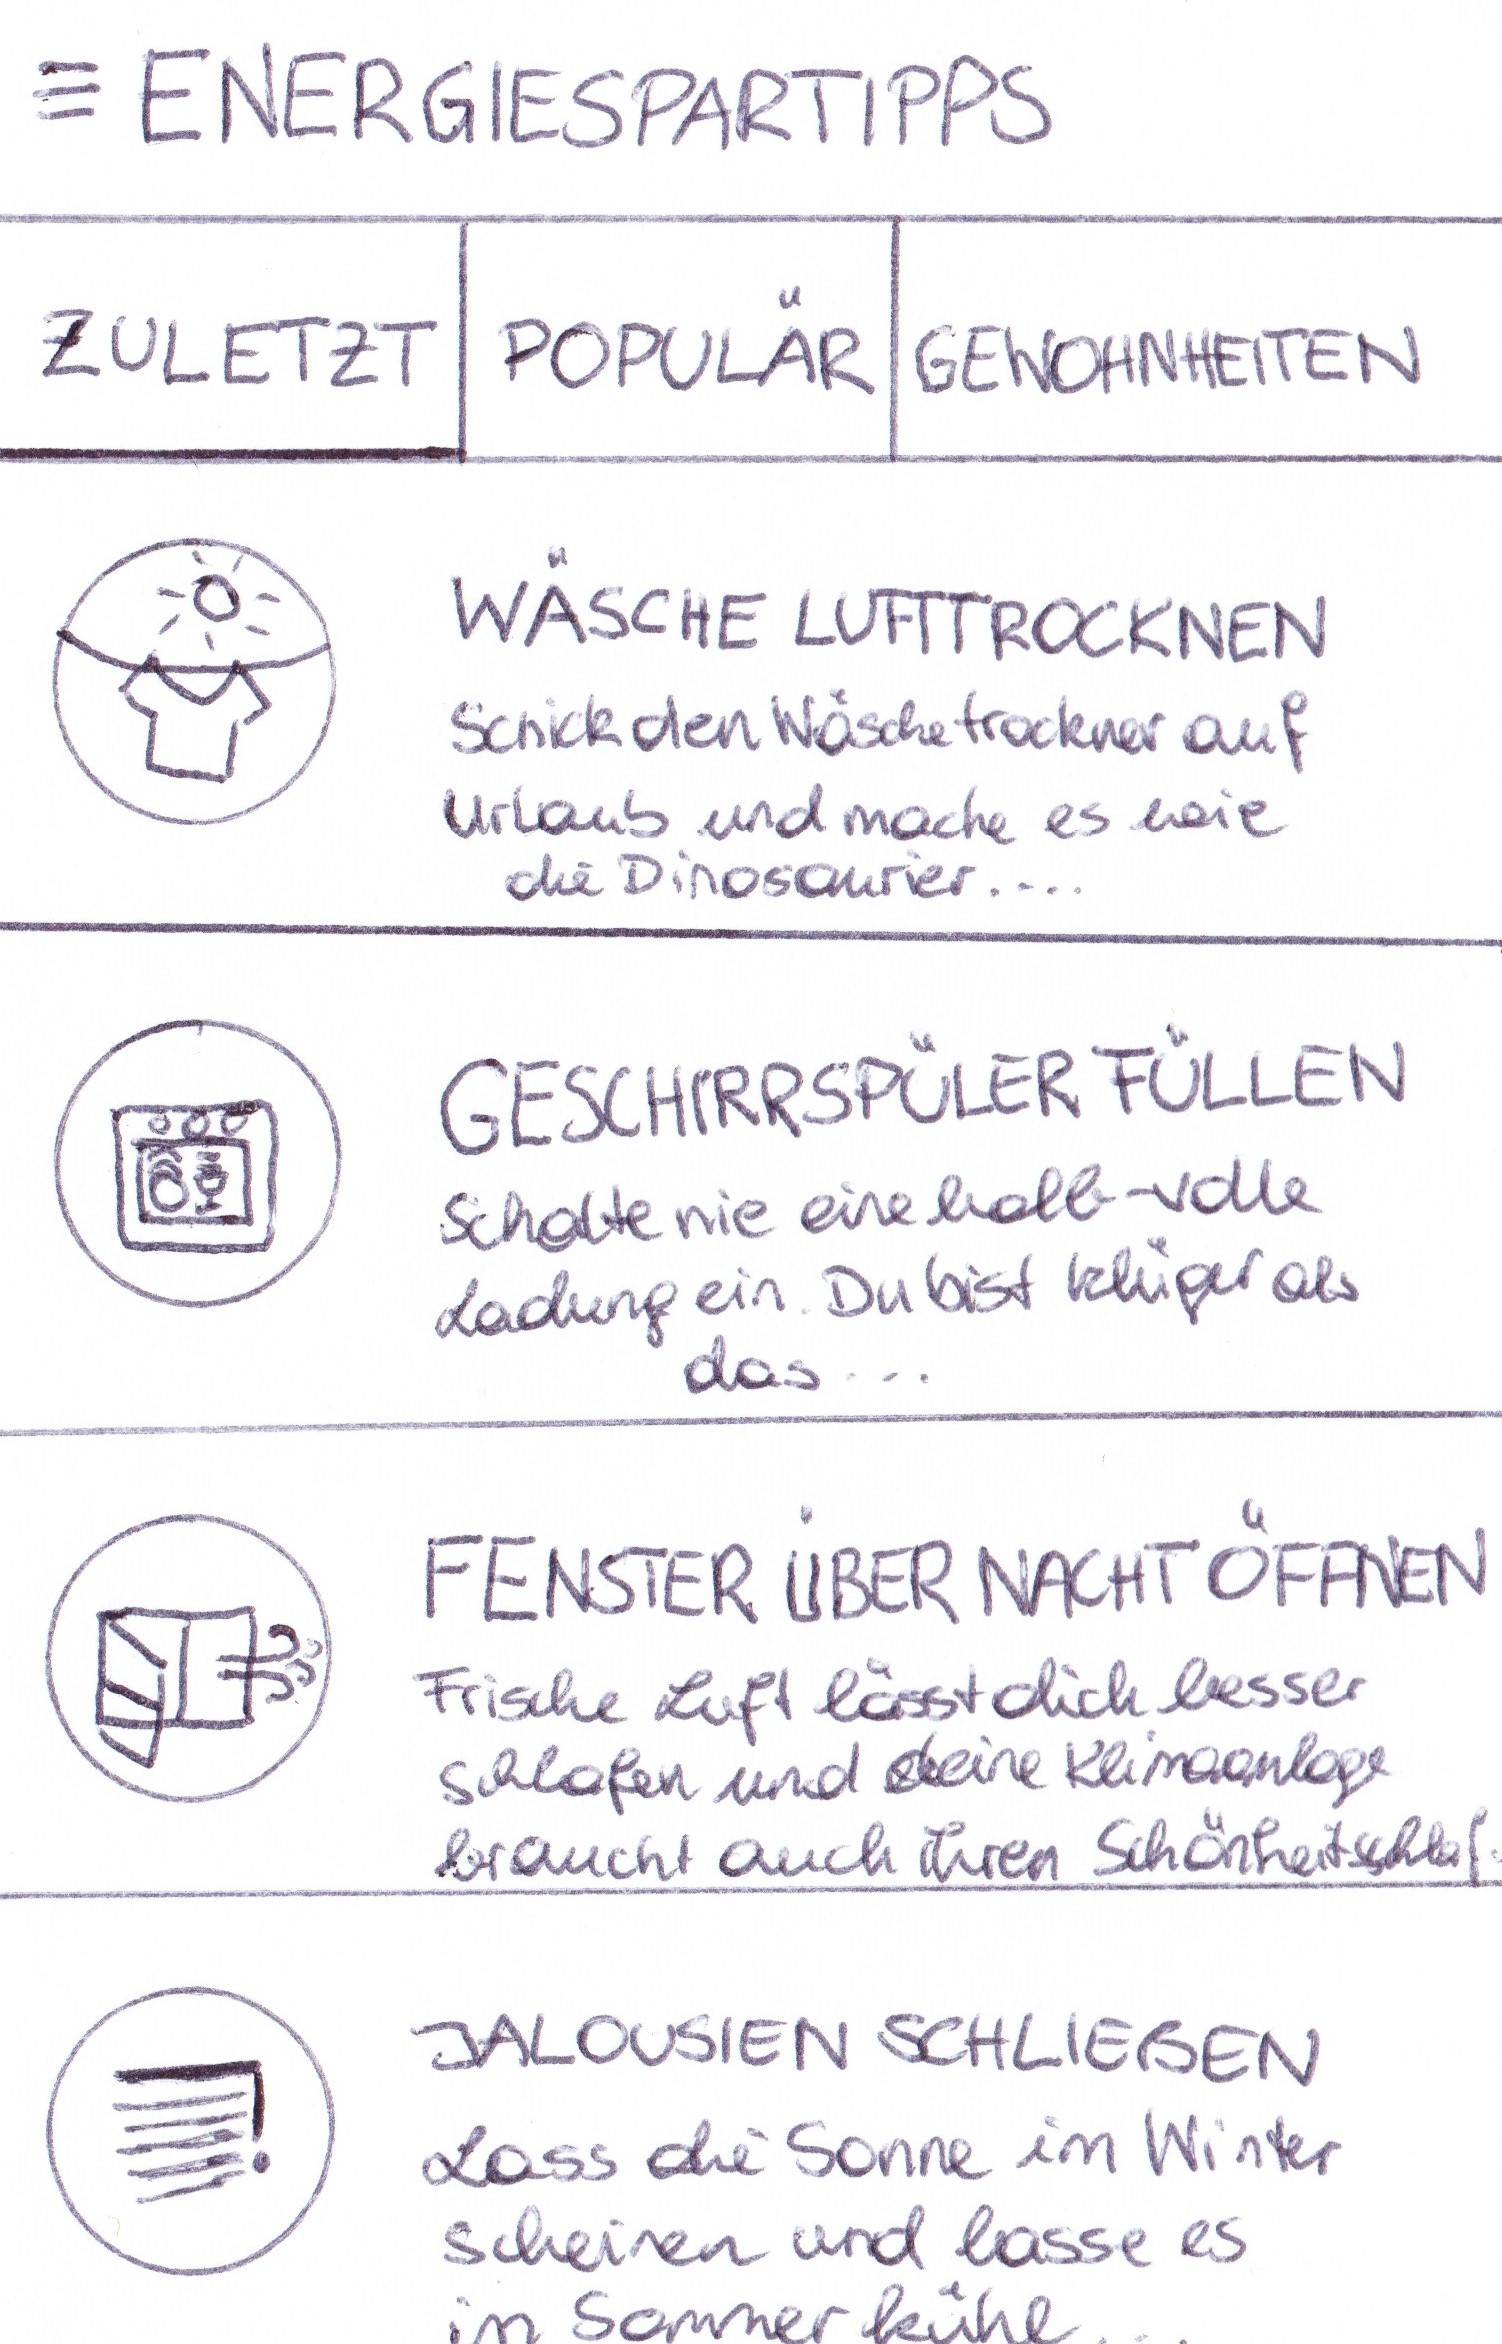
\includegraphics[width=\textwidth]{screens/tipp_1}
		\subcaption{Professional}
		\label{fig:tipps:professional}
	\end{subfigure}
	\begin{subfigure}[b]{0.24\columnwidth}
		\centering
		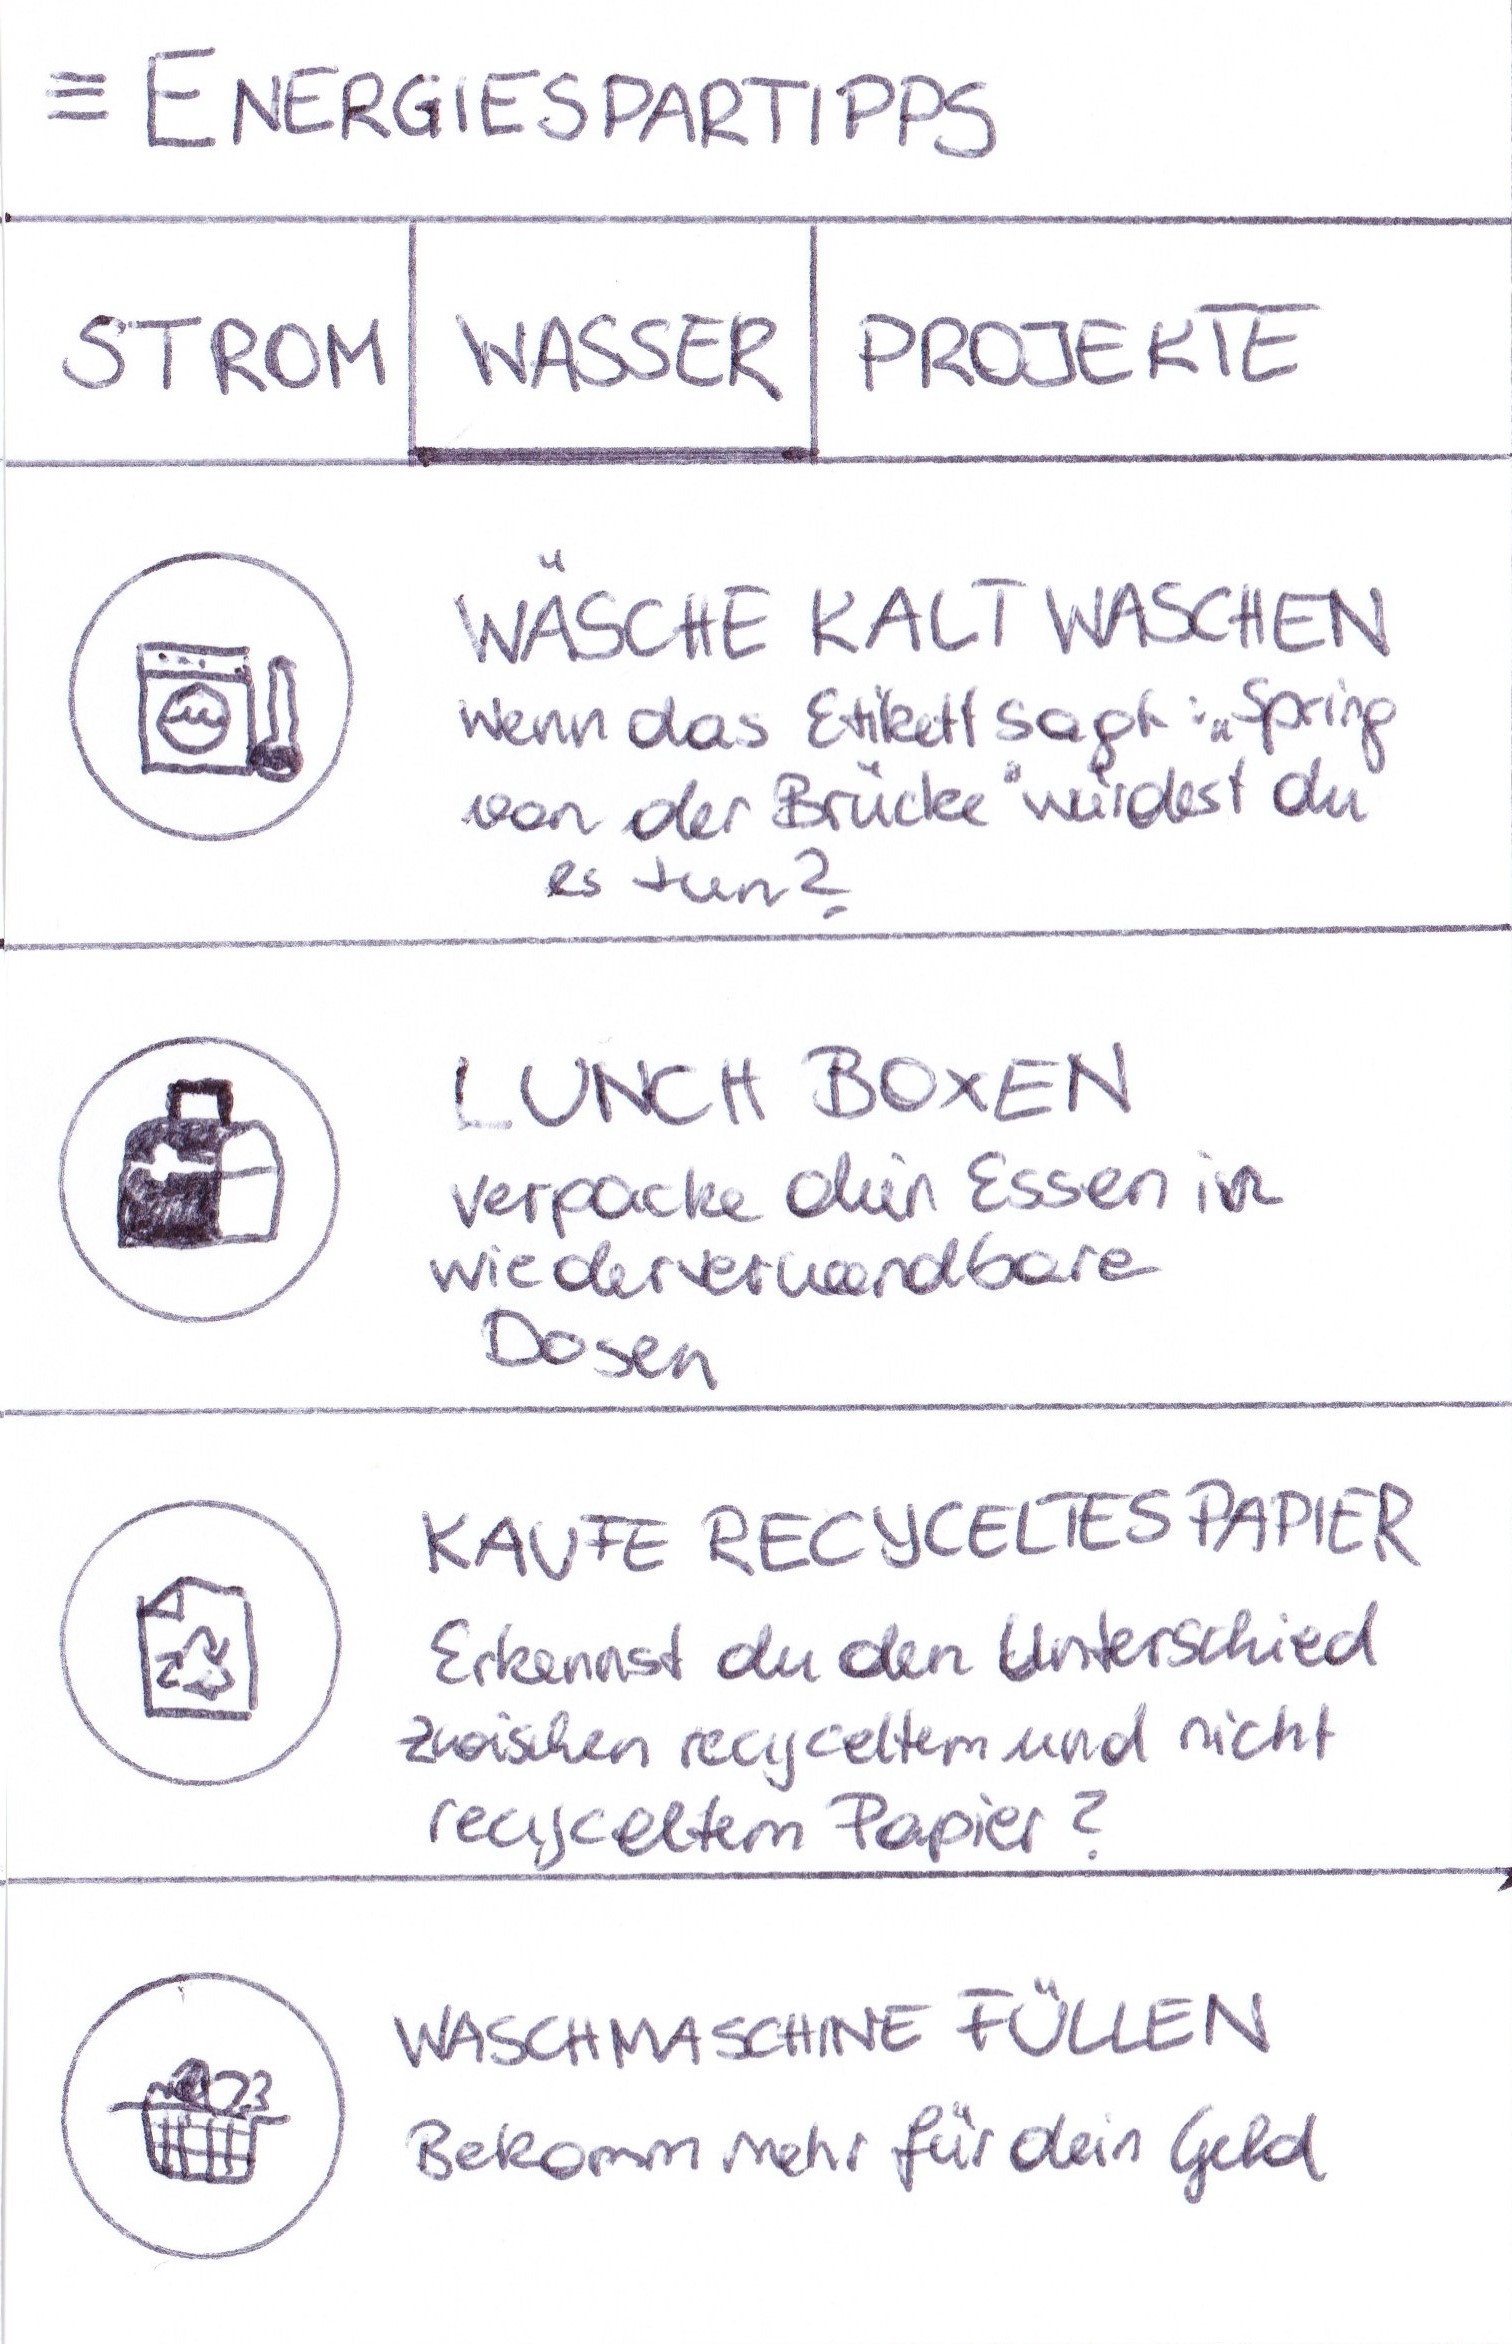
\includegraphics[width=\textwidth]{screens/tipp_2}
		\subcaption{Optimizer}
		\label{fig:tipps:optimizer}
	\end{subfigure}
	\begin{subfigure}[b]{0.24\columnwidth}
		\centering
		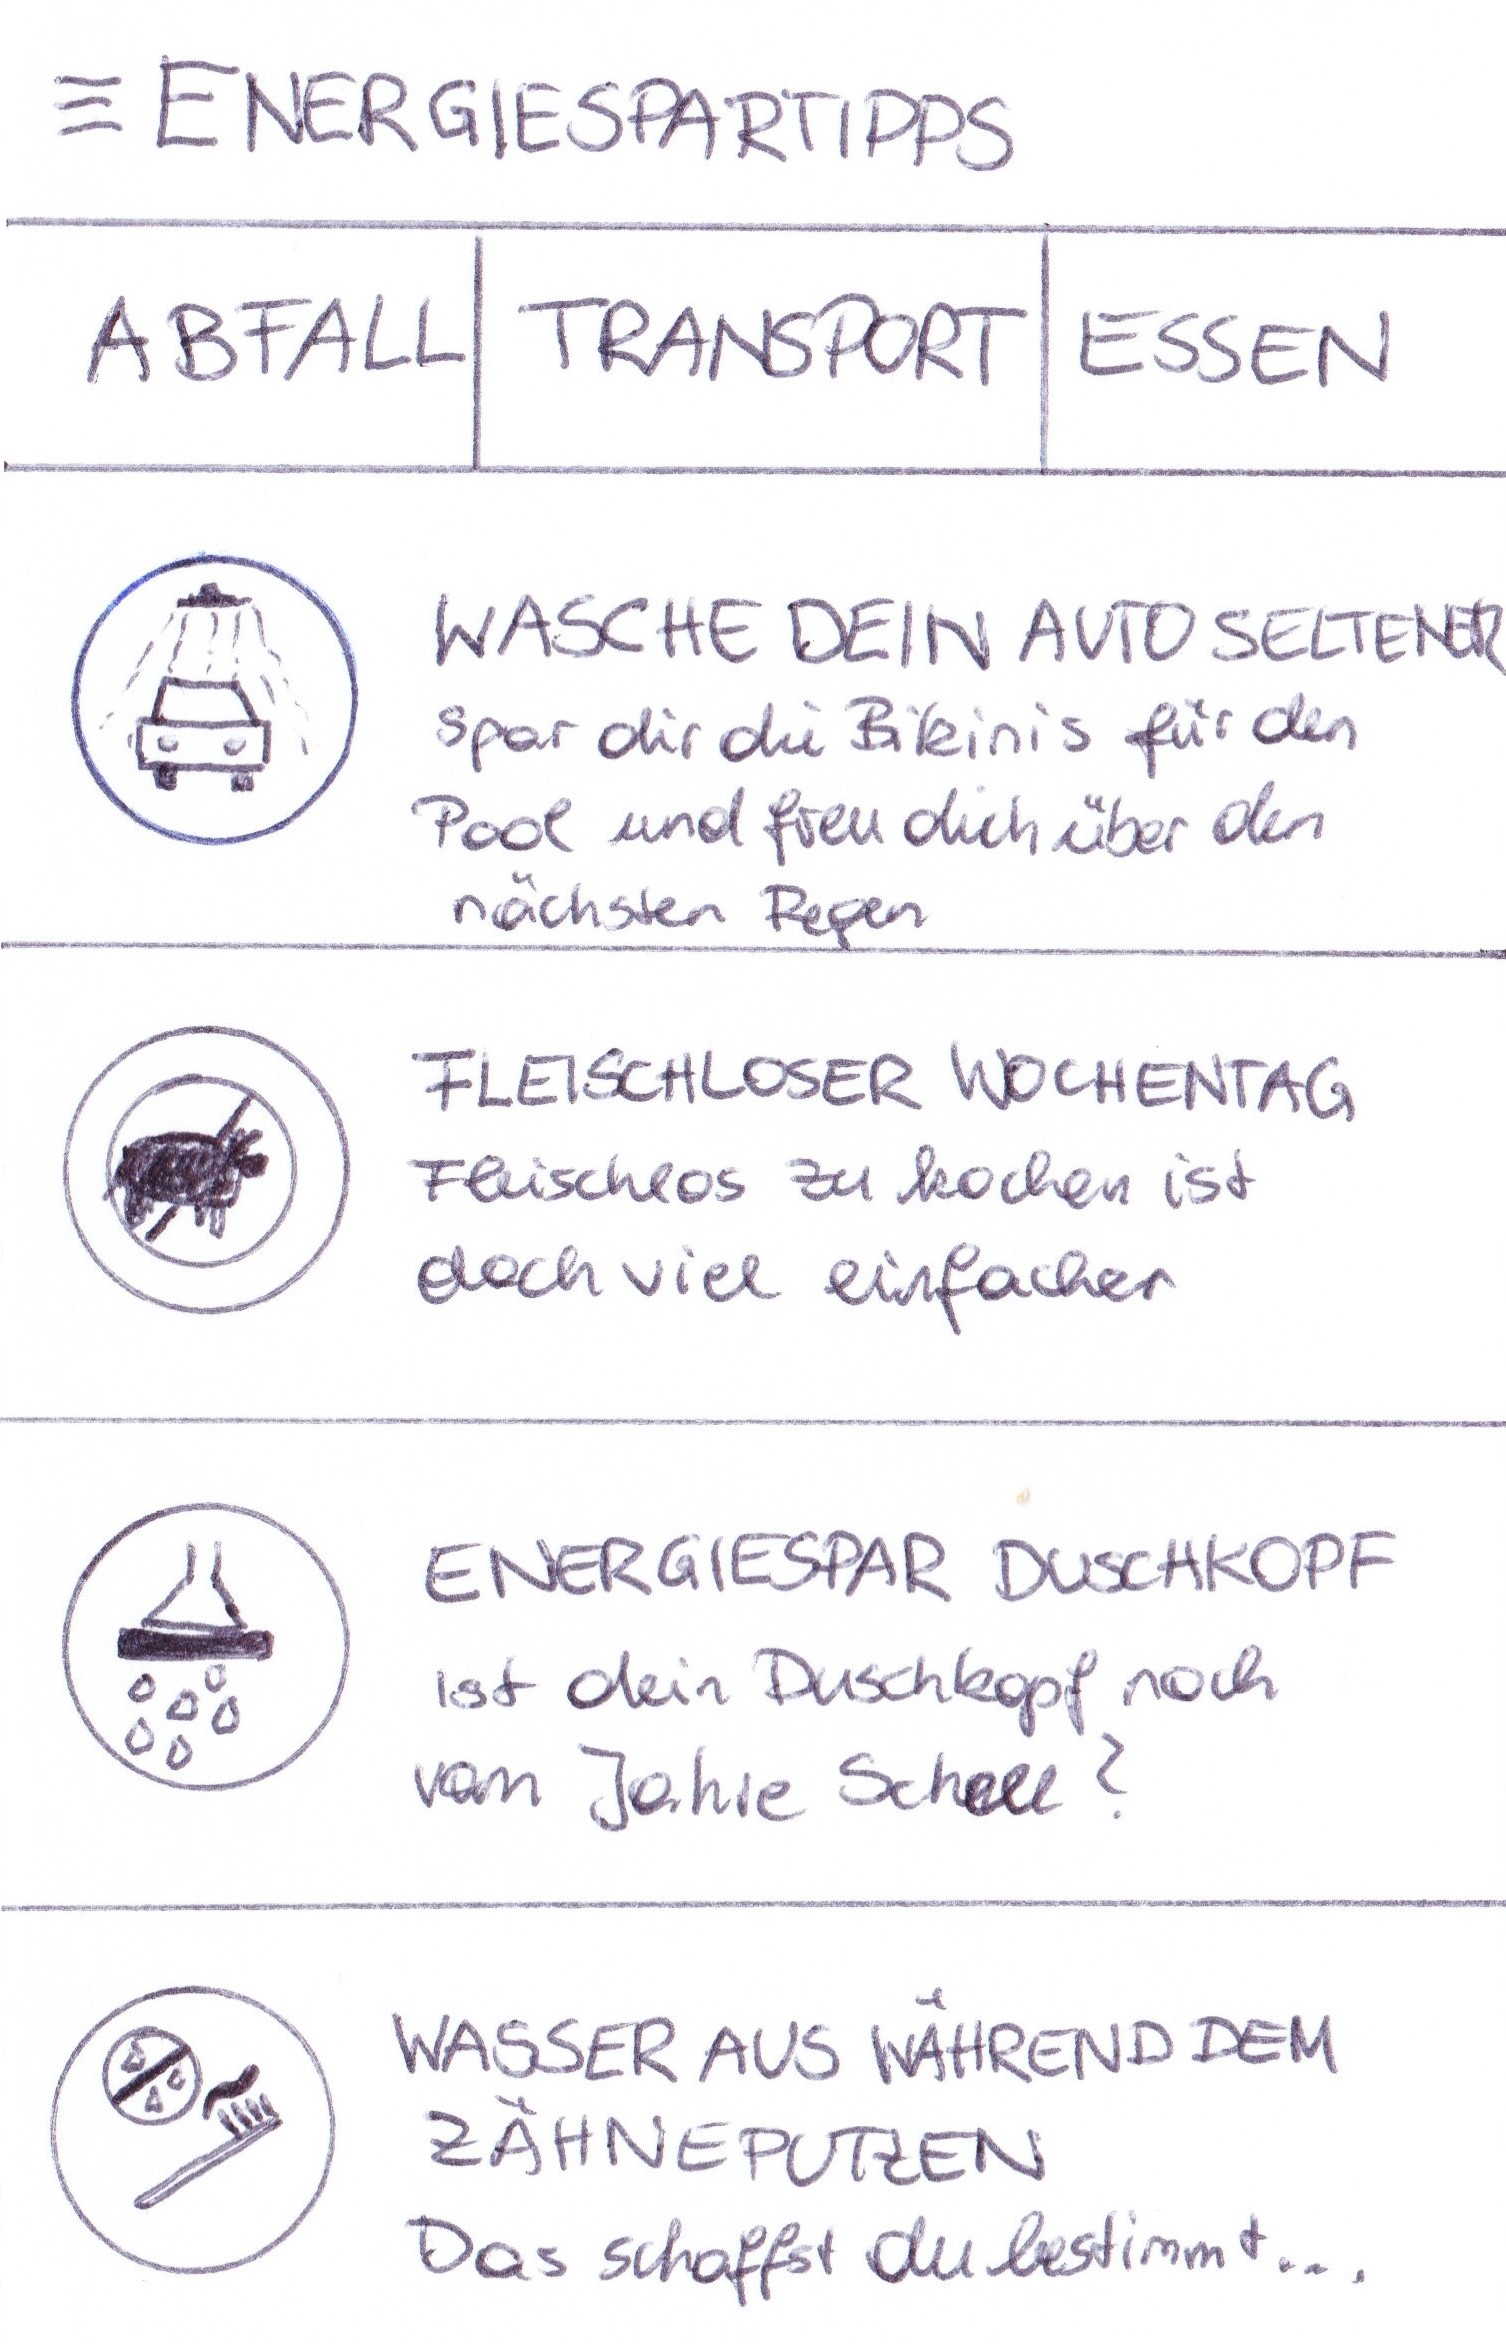
\includegraphics[width=\textwidth]{screens/tipp_3}
		\subcaption{Indifferent}
		\label{fig:tipps:indifferent}
	\end{subfigure}
	\begin{subfigure}[b]{0.24\columnwidth}
		\centering
		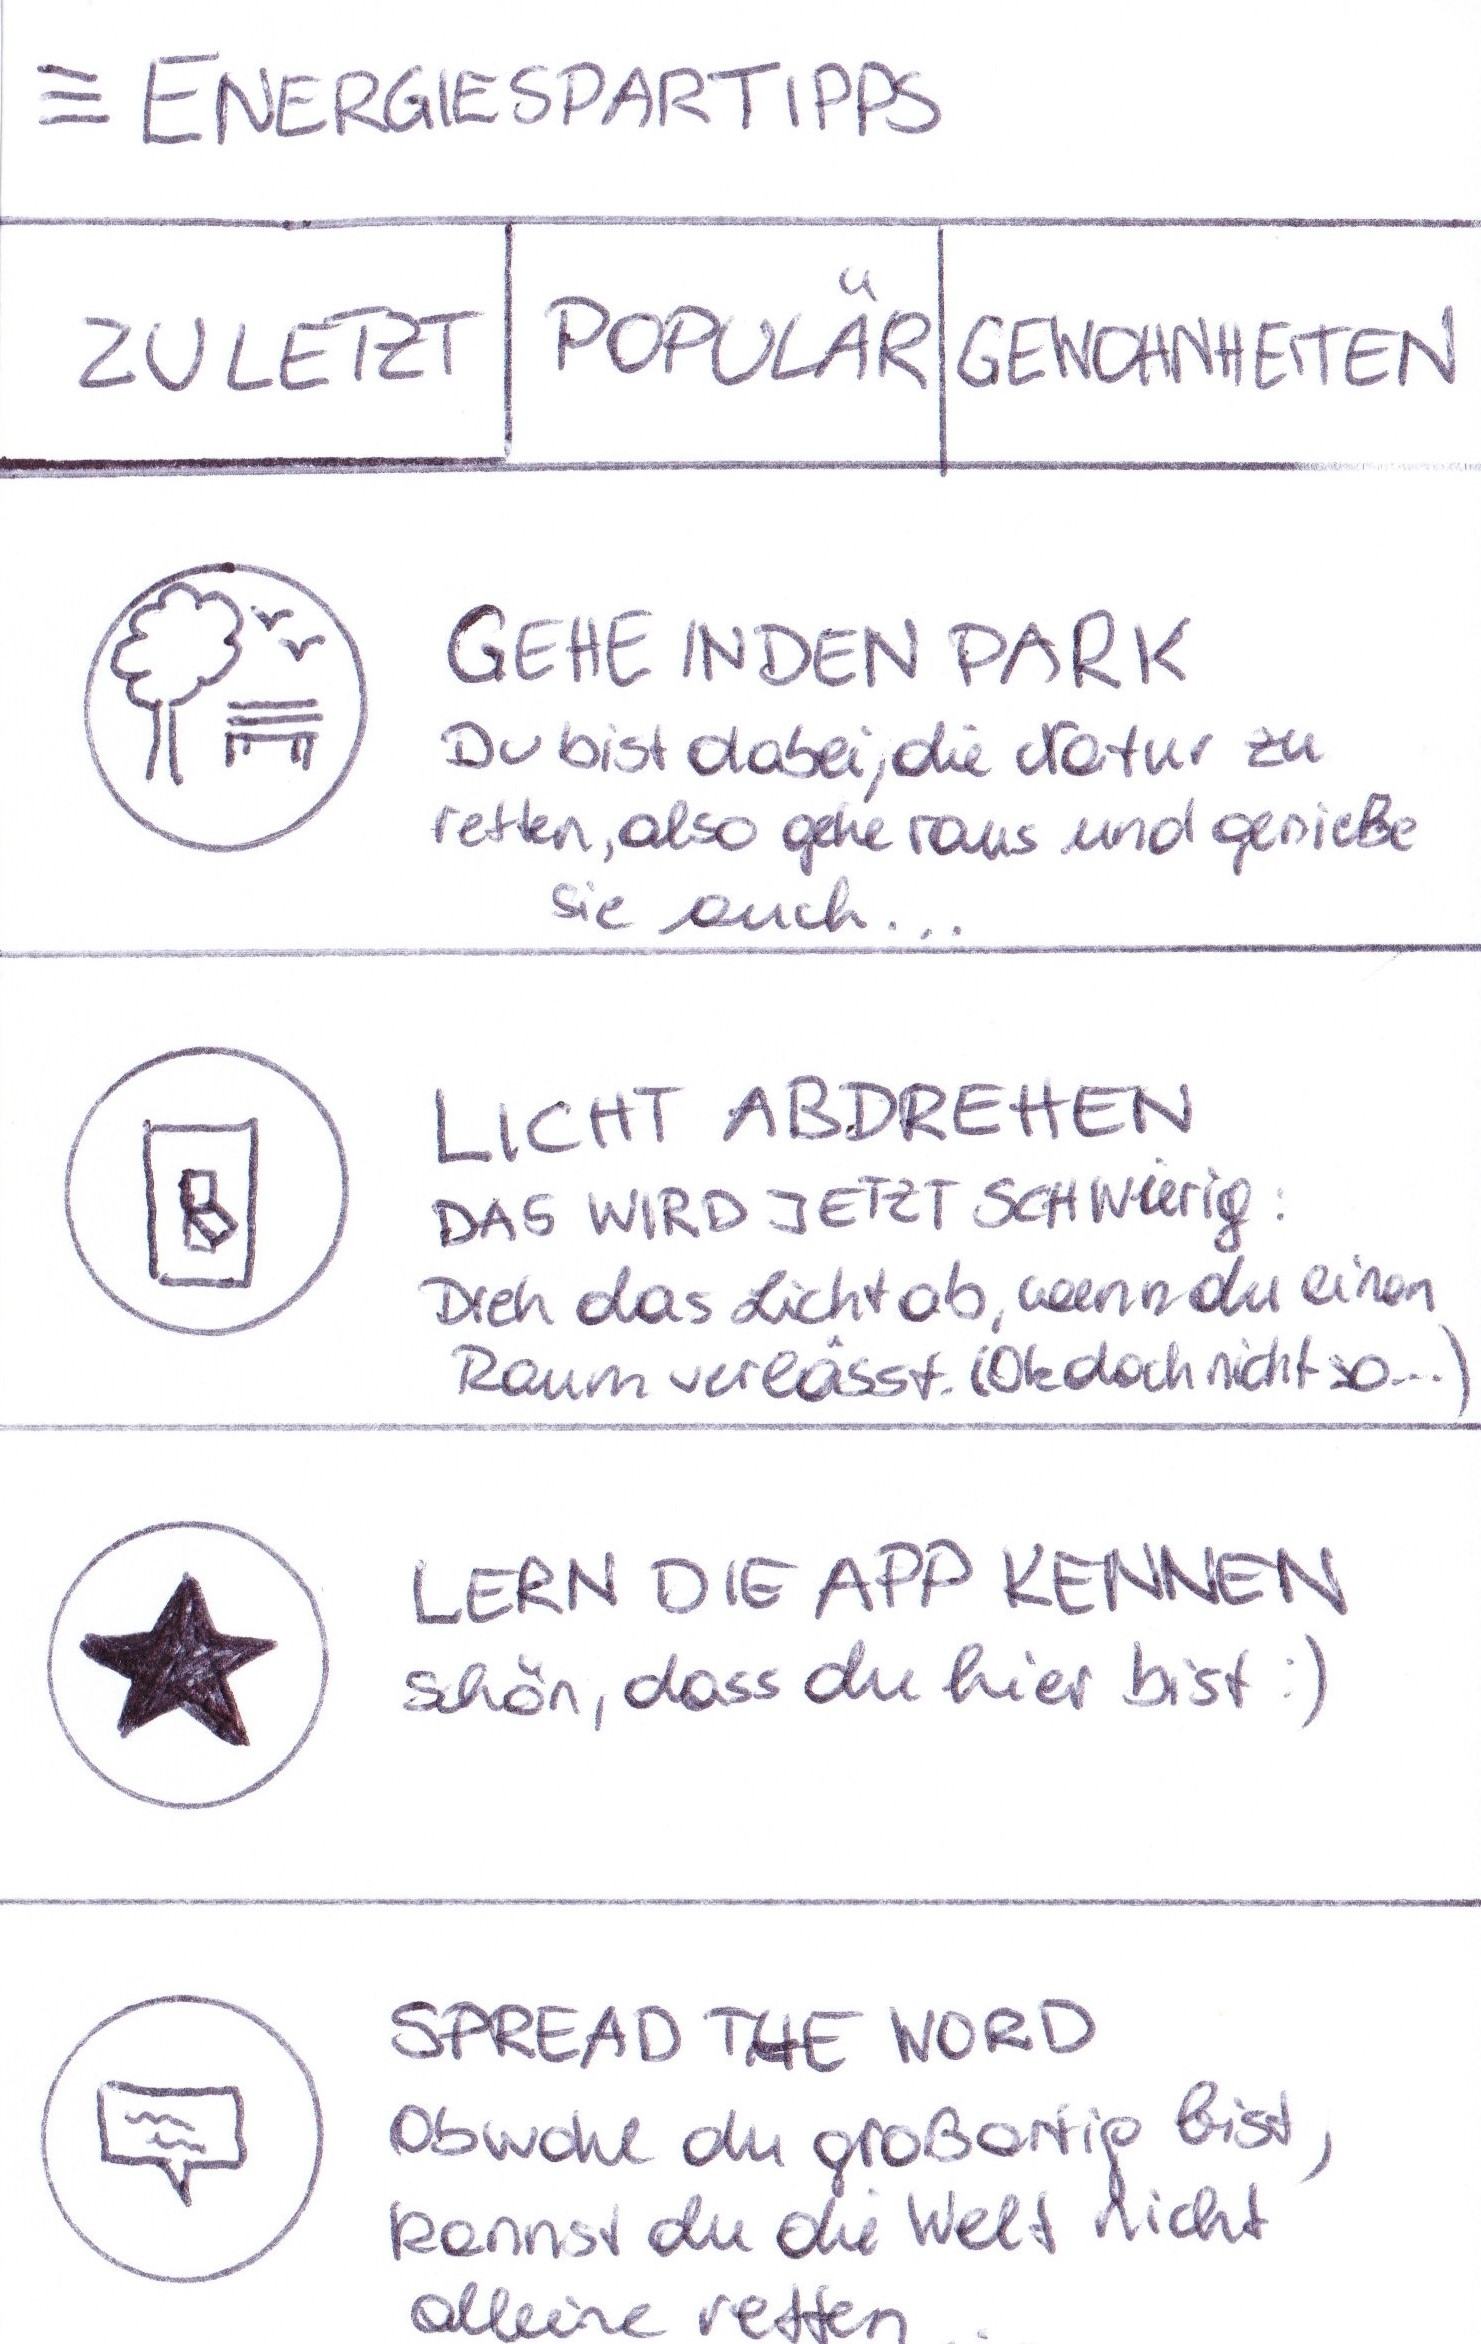
\includegraphics[width=\textwidth]{screens/tipp_4}
		\subcaption{Hedonist}
		\label{fig:tipps:hedonist}
	\end{subfigure}
	\caption{The paper prototype screen for energy saving tips}
	\label{fig:tipps} % \label has to be placed AFTER \caption (or \subcaption) to produce correct cross-references.
\end{figure}

\section{Gamification approach}
 Indifferents are interested in energy saving tips more if they can success in the game
\begin{figure}[h]
	\centering
	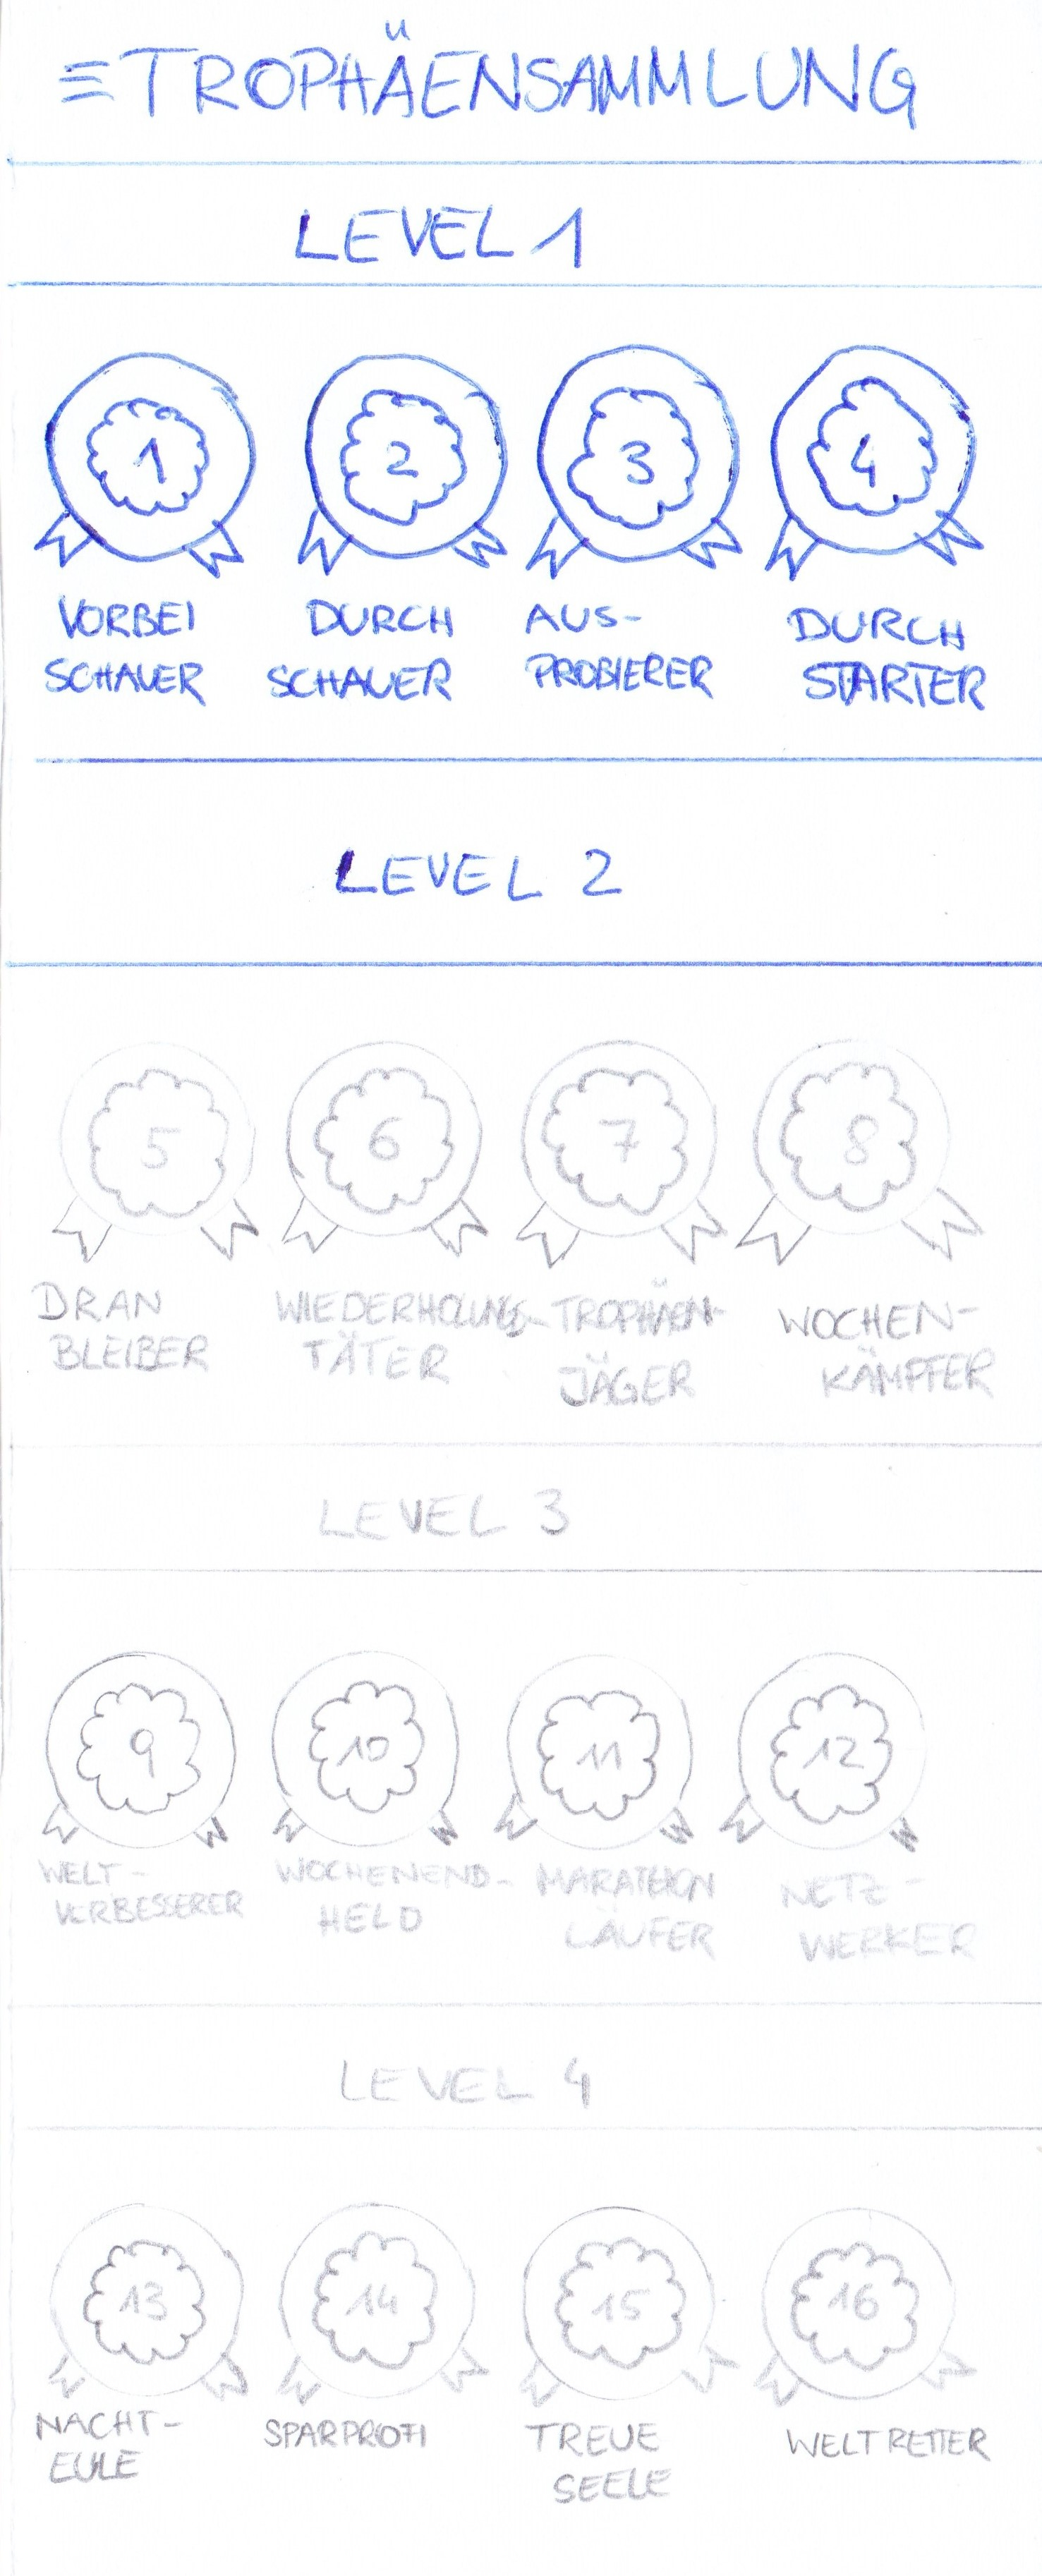
\includegraphics[width=0.24\columnwidth]{screens/Trophaensammlung}
	\caption{The proposed screens for trophy}
	\label{fig:trophaen} % \label has to be placed AFTER \caption (or \subcaption) to produce correct cross-references.
\end{figure}

\section{Trouble Shooting}
Present a hotline for trouble shooting for optimizer/Optimizer prefer calling when an error occurs
Present FAQs before telephone number for Hedonists and Indifferents and Professionals

\begin{figure}[h]
	\centering
	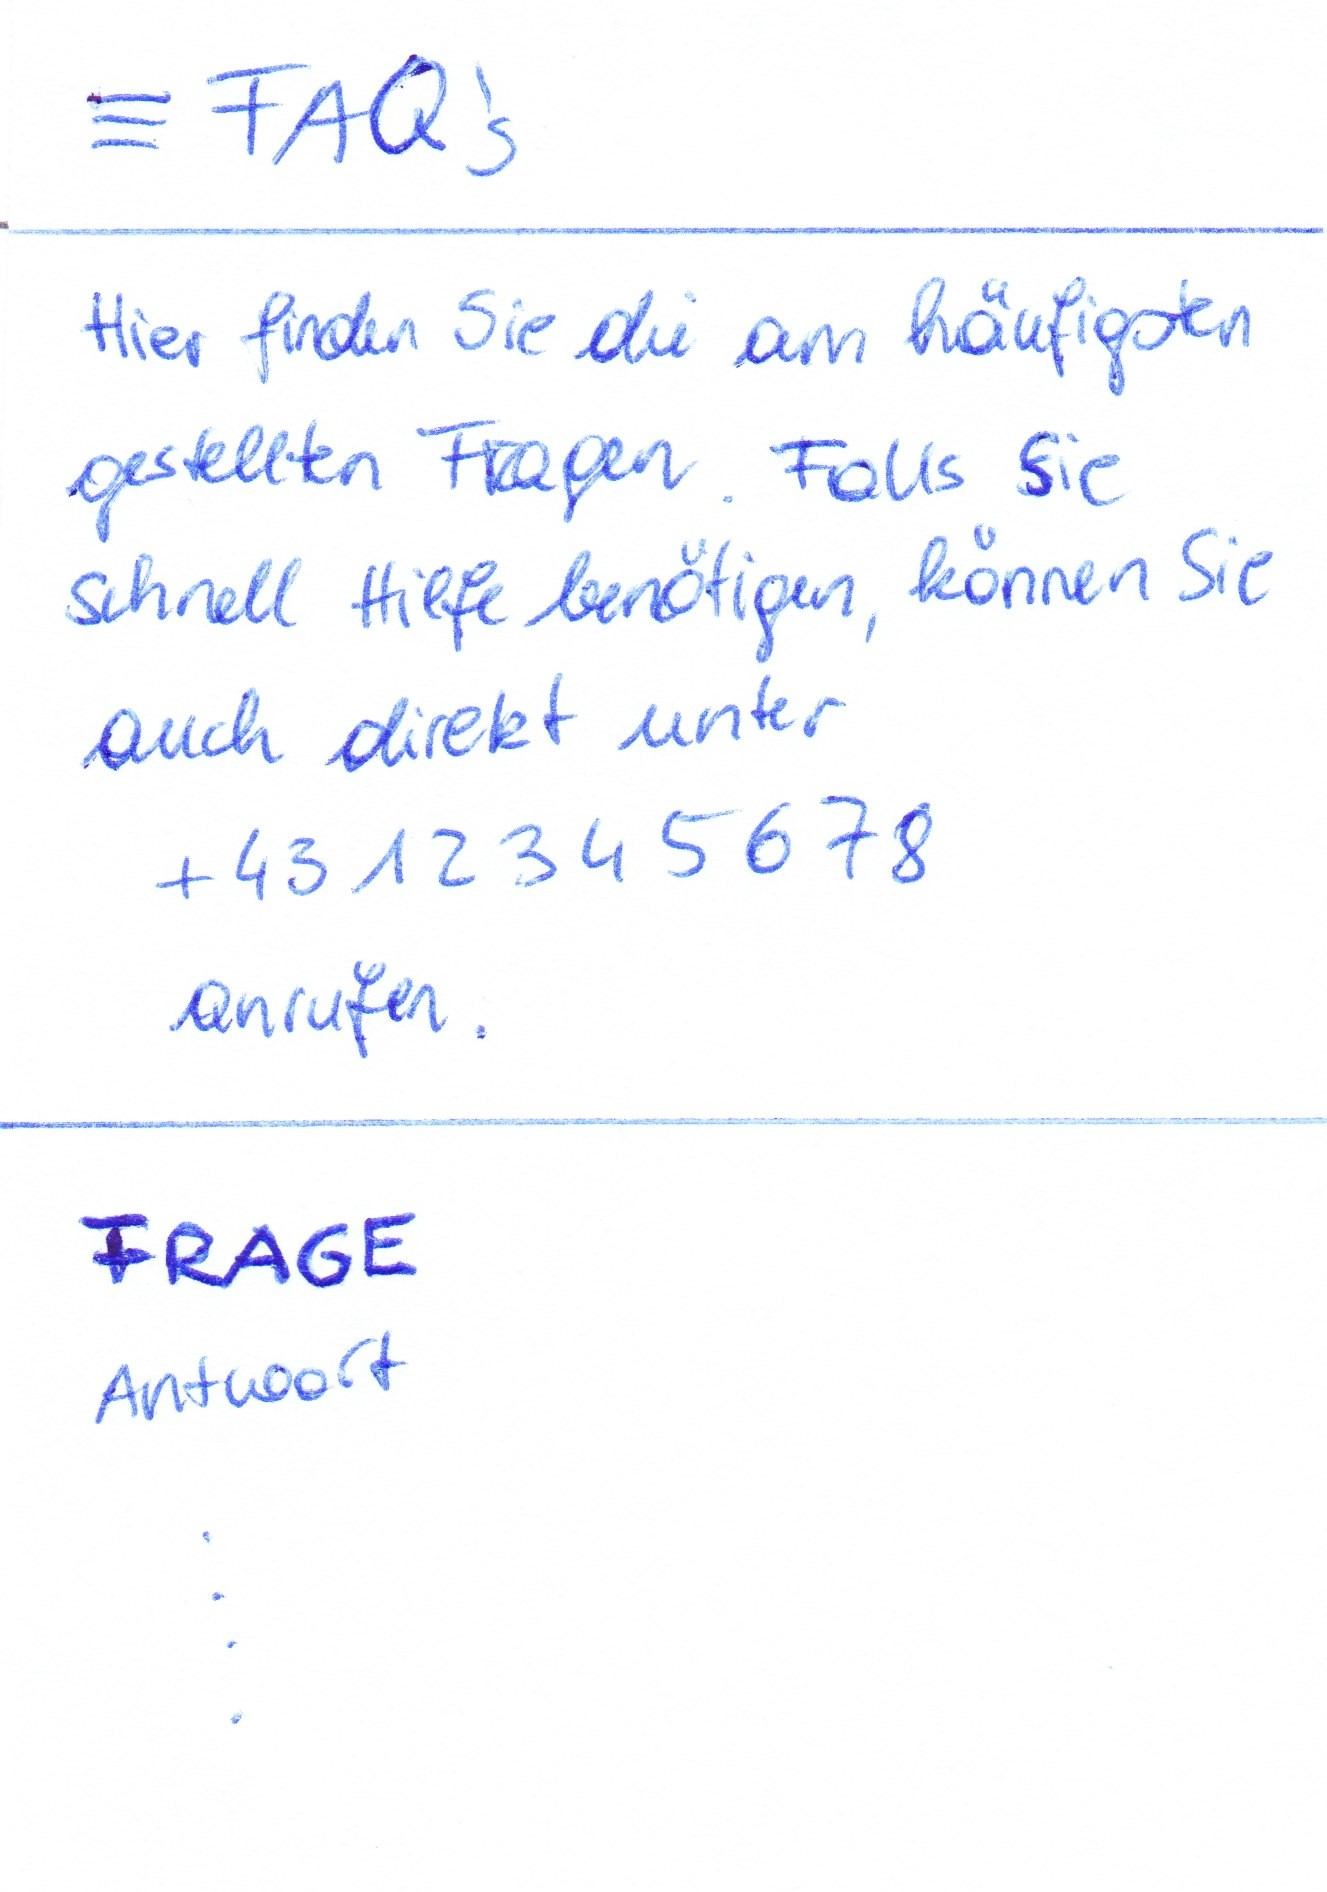
\includegraphics[width=0.24\columnwidth]{screens/FAQs}
	\caption{The proposed screens for Trouble shooting}
	\label{fig:trouble} % \label has to be placed AFTER \caption (or \subcaption) to produce correct cross-references.
\end{figure}





\section{Communication}
Hedonists prefer praise 
Use concrete instruction for Optimizer and avoid detailed information/Optimizer prefer concrete instructions to detailed information



\subitem{\textbf{Professionals}}: The user study revealed that Professionals have high interest in energy issues. As they are deep into the topic and prefer more detailed information in individual offers they can have a look on the energy consumption on a very detailed level, such as a consumption rate on a granularity of minutes. Professionals also should have a possibility within the application to compare energy consumptions of different time intervals. According to the user study Professionals also like to compare themselves to others. Professionals also like rationally justified explanations and instructions for use. Notifications should give tips on saving energy or CO2, give concrete instructions for use and provides deeper information in Energy topics. This results in the following tasks for professionals:



\subitem{\textbf{Optimizer}}: Optimizer primarily aim at optimizing energy costs, so the app should give easy to find tips on how to save energy and therefore costs. Optimizers also prefer less time of interaction and rather like unclear instructions. Therefore the notifications also should give concrete instructions on how to save energy or CO2. Optimizer also like to know the concrete benefits of a certain behaviour change. The explanations shall be as close to reality as possible and technical language shall be avoided. The energy feedback is reduced to essential information and the detailed graphs for energy consumption that the Professionals get, should not be visible at a first glance for an Optimizer. The saved costs after a behaviour change shall also be visible to provide some kind of reward for the new habits. For Optimizer also trouble shooting shall be easily accessible, in order to reduce the time they are spending with the application and not to loose them on the way.



\subitem{\textbf{Indifferents}}:
The Indifferents have low interest in energy topics in general, so the main requirement of the application for this type of user is in the first run to sensitize them for the topic, to raise awareness and to make electricity and CO2 saving appealing to them. To awaken their interest for energy and sustainability a gamification approach will be used. For opening the application once a day the user earns points. Points are also earned for clicking on notifications and reading the article. Tips for saving energy or CO2 should not concern longer usage of laptops or entertainment screens, as streaming and use of social media is an important leisure activity for Indifferents.


\subitem{Hedonists}:
The youngest segment, the Hedonists, are keen on developing technical solutions. The interest in technology can be used to give instructions for programming technical devices and using home automation. The primary motive for the Hedonists is not to save energy but the interest in technology. This will be considered in the notifications and tips of the day. The hedonistic lifestyle with its strong convenience and comfort orientation is in the foreground. For a hedonist the comfort gain is of great relevance. Programming and establishing home automation aspects is a great interface between the aim of saving energy and the affinity of technology.


el be shown in a dashboard, in about how much electricity, water and heating a user consumed, how much carbon-dioxide was produced and how the values can be made better in the sense of reducing consumptions. The screens shall be adapted to the user type to make the information and tips more attractive to a user's interests. The interfaces shall be different for each user but every user should basically have the possibility to do all tasks.

\begin{enumerate}
	\item As a user I want to have a look on your consumption rate of the last day/week/month/year
	\item Compare your consumption rate of the last day/week/month/year with the consumption rate of the same week one year earlier.
	\item Compare your consumption rate of the last week with the average consumption rate of your neighbours
	\item Find tips on how to save more energy
	\item Find out what to do to save costs for electricity
	\item Find out how much you have saved in the last week
	\item Earn trophies by interacting with the App
	\item Start a project to install a home automation gadget that saves energy in the long run
	\item Report a problem
\end{enumerate}



In order to elicit the requirements for the graphical user interfaces and to find usability mistakes we make use of Paper Prototyping. 


\section{Design Guidelines for tailoring interfaces to user segments}

\section{Recommendations for improvement for the ASCR App}

\begin{figure}[h]
	\centering
	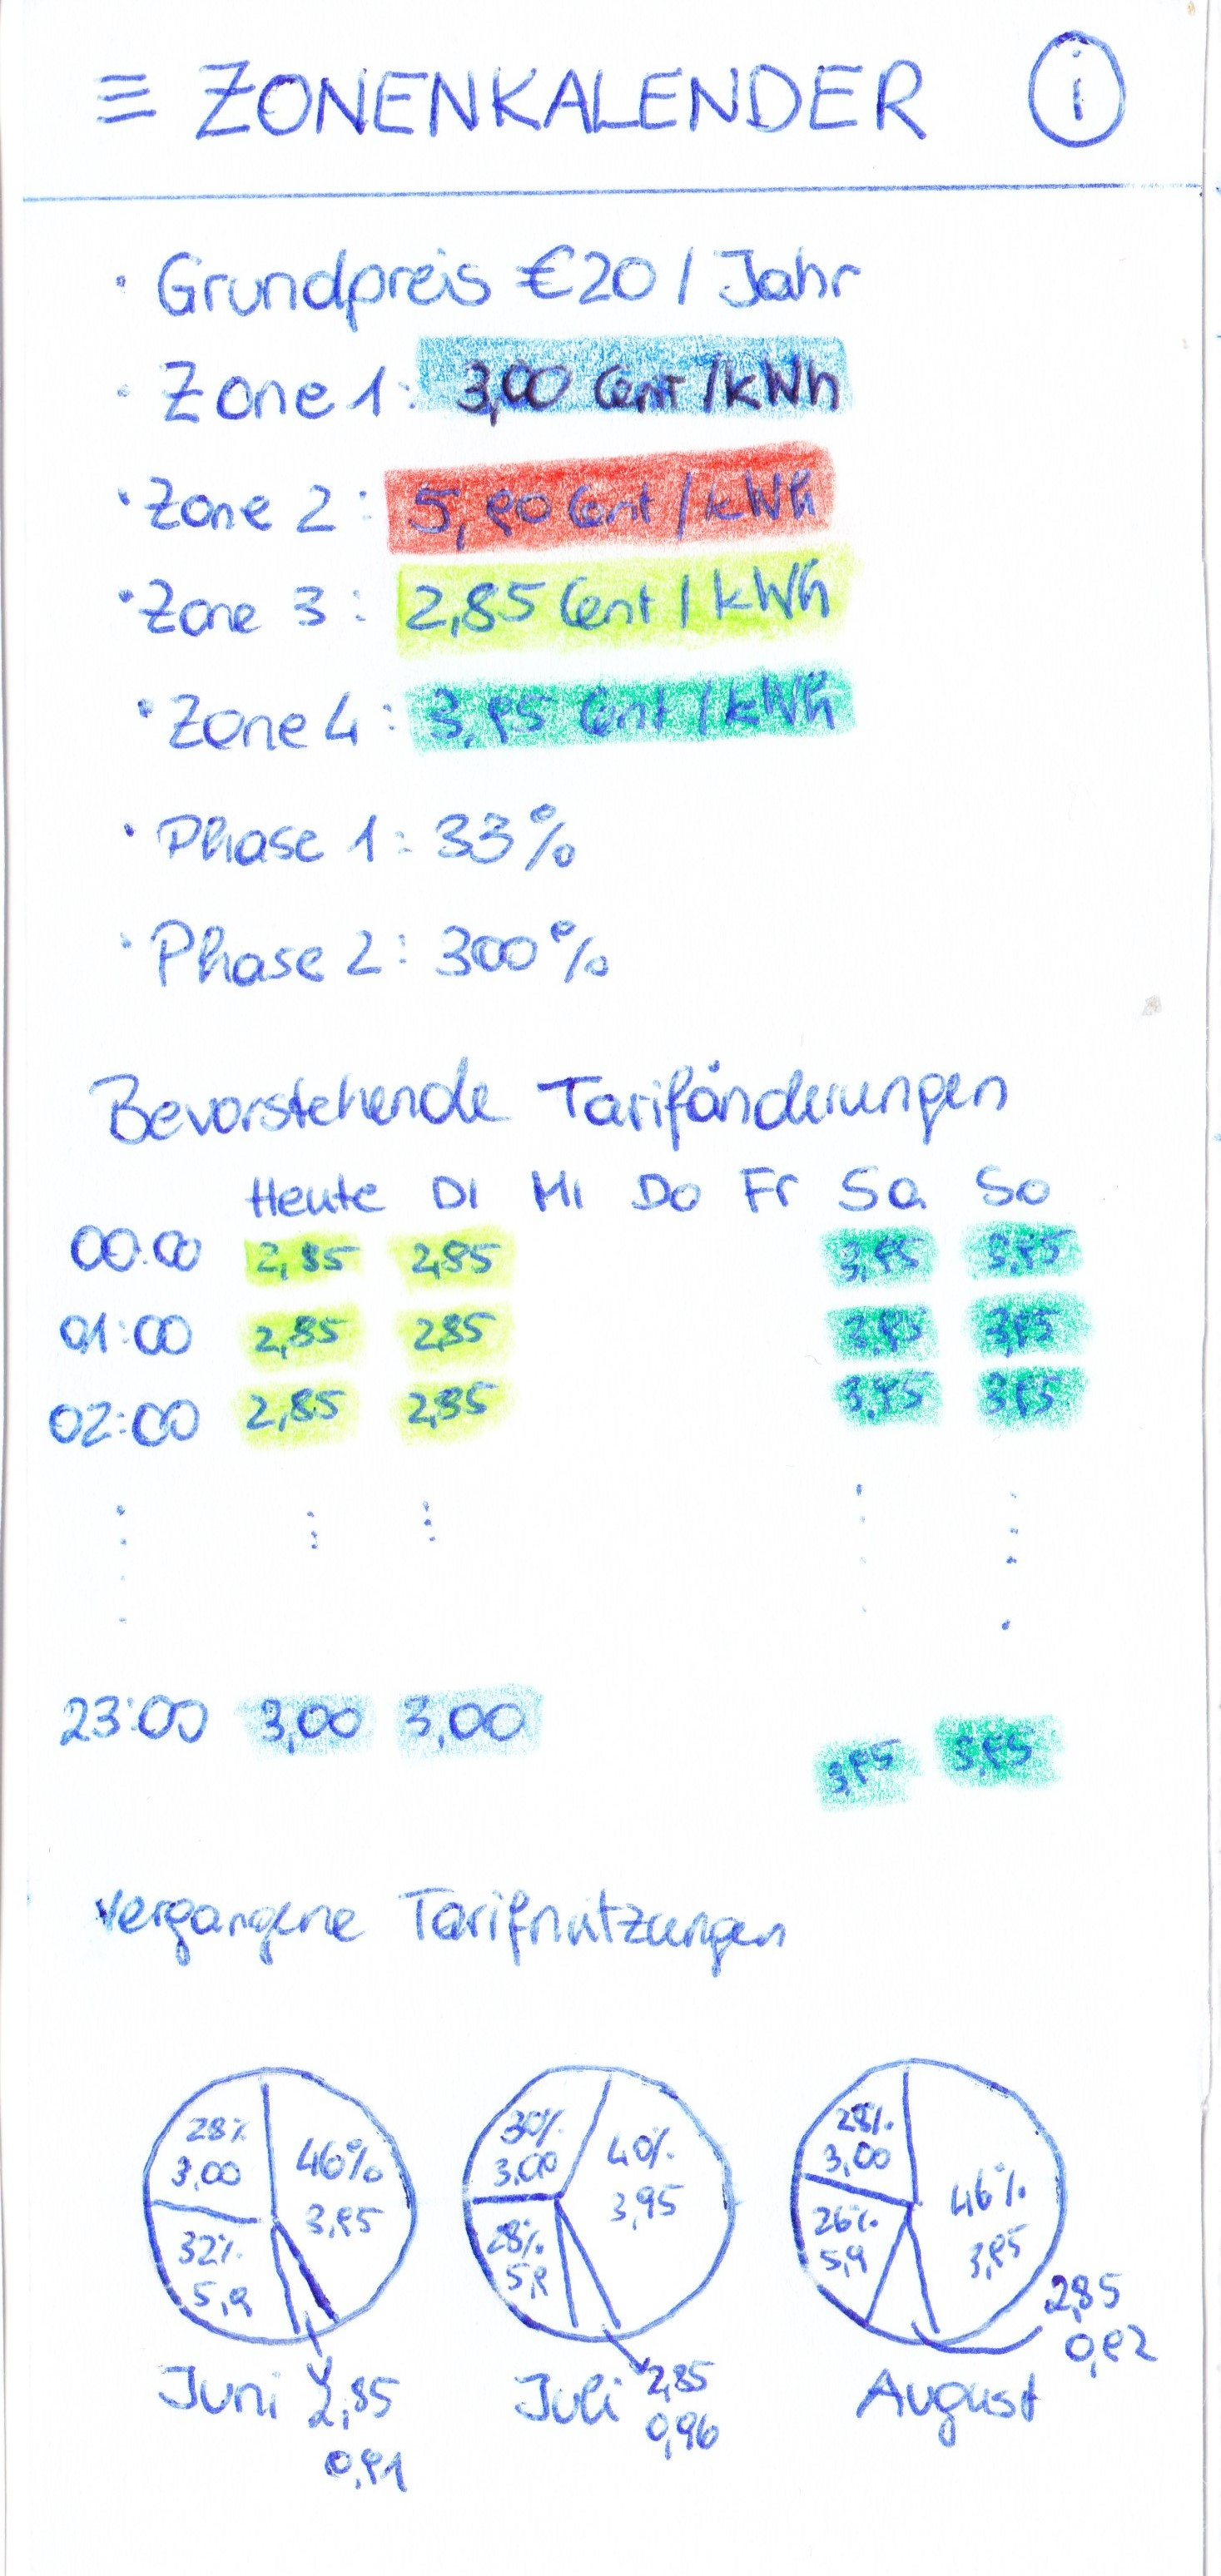
\includegraphics[width=0.24\columnwidth]{screens/Zonenkalender}
	\caption{A recommendation for the tariff description }
	\label{fig:kalender} % \label has to be placed AFTER \caption (or \subcaption) to produce correct cross-references.
\end{figure}

